\documentclass[12pt,a4paper]{report}

% ── Encodage & langue ──────────────────────────────────────────────────────────
\usepackage[utf8]{inputenc}
\usepackage[T1]{fontenc}
\usepackage[french]{babel}
% Police Times New Roman 12 pt (consigne ESPRIT — note pédagogique)
\usepackage{mathptmx}

% ── Mise en page ───────────────────────────────────────────────────────────────
% Marges 2,5 cm (consigne ESPRIT)
\usepackage[a4paper, top=2.5cm, bottom=2.5cm, left=2.5cm, right=2.5cm]{geometry}
\usepackage{setspace}
% Interligne 1,15 (consigne ESPRIT)
\setstretch{1.15}

% ── En-tête / pied de page ─────────────────────────────────────────────────────
\usepackage{fancyhdr}
\pagestyle{fancy}
\fancyhf{}
\fancyhead[L]{\small\textbf{3S TalentMatch}}
\fancyhead[R]{\small\nouppercase{\leftmark}}
% Numéro de page en bas à droite (consigne ESPRIT)
\fancyfoot[R]{\thepage}
\renewcommand{\headrulewidth}{0.4pt}
% Première page des chapitres : même pagination en bas à droite
\fancypagestyle{plain}{%
  \fancyhf{}%
  \fancyfoot[R]{\thepage}%
  \renewcommand{\headrulewidth}{0pt}%
}

% ── Chapitres (style Sirine) ───────────────────────────────────────────────────
\usepackage{titlesec}
\usepackage{xcolor}
\definecolor{chaptercolor}{RGB}{0,0,0}

\titleformat{\chapter}[display]
  {\normalfont\Large\bfseries}
  {\filleft\large Chapitre \thechapter}
  {0pt}
  {\titlerule[1pt]\vspace{6pt}\filright\huge}
  [\vspace{6pt}\titlerule]

\titlespacing*{\chapter}{0pt}{-10pt}{30pt}

% ── Packages utiles ────────────────────────────────────────────────────────────
\usepackage{graphicx}
\usepackage{pdfpages}
\usepackage{booktabs}
\usepackage{colortbl}
\definecolor{tabheader}{RGB}{27,79,138}
\definecolor{tabalt}{RGB}{240,244,249}
\usepackage{tabularx}
\usepackage{array}
\usepackage{longtable}
\usepackage{enumitem}
\usepackage{float}
\usepackage{framed}
\usepackage{pifont}   % \ding{51} : coche dans les matrices de permissions
% (la classe report numérote déjà figures et tableaux par chapitre)

% ── Liens cliquables (TOC, listes des figures/tableaux, références) ────────────
% hidelinks : liens actifs mais sans cadres rouges à l'impression
\usepackage[hidelinks]{hyperref}

% ═══════════════════════════════════════════════════════════════════════════════
\begin{document}

% ── Pages préliminaires : page de garde ESPRIT + page de validation ───────────
\includepdf[pages=1-2]{pages_preliminaires.pdf}

% ── Dédicaces ─────────────────────────────────────────────────────────────────
\chapter*{Dédicaces}
\addcontentsline{toc}{chapter}{Dédicaces}
\thispagestyle{empty}

\vspace{1.5cm}
\begin{center}
\textit{Je dédie ce travail}\\[16pt]
\textit{À \textbf{ma très chère mère},\\
source inépuisable d'amour, de patience et de tendresse,\\
dont les prières et les sacrifices m'ont accompagné à chaque pas.\\
Aucun mot ne saurait exprimer ma gratitude.}\\[14pt]
\textit{À \textbf{mon très cher père},\\
mon exemple de courage et de persévérance,\\
qui n'a jamais cessé de croire en moi et de me soutenir\\
pour que je devienne ce que je suis aujourd'hui.}\\[14pt]
\textit{À \textbf{ma chère s\oe ur},\\
pour son affection, son soutien indéfectible\\
et ses encouragements dans les moments de doute.}\\[14pt]
\textit{À \textbf{toute ma famille} et à \textbf{mes amis},\\
pour leur présence et leurs encouragements constants.}\\[14pt]
\textit{Que ce travail soit le témoignage\\
de ma profonde reconnaissance et de mon amour.}\\[1.5cm]
\hfill \textit{Youssef GARA}
\end{center}
\newpage

% ── Remerciements ─────────────────────────────────────────────────────────────
\chapter*{Remerciements}
\addcontentsline{toc}{chapter}{Remerciements}

C'est avec un profond sentiment de gratitude que j'adresse ces quelques mots à toutes les personnes qui, par leur encadrement, leur confiance ou leur affection, ont contribué à l'aboutissement de ce projet de fin d'études.

Mes remerciements s'adressent en premier lieu à mon encadrante en entreprise, \textbf{Madame Sirine Nasri}, ingénieure au sein de \textbf{3S Group}, pour la qualité exceptionnelle de son encadrement : sa disponibilité constante, la pertinence de ses conseils, son exigence bienveillante et la confiance qu'elle m'a accordée tout au long de ce stage ont été déterminantes dans la réussite de ce projet.

J'exprime également ma sincère reconnaissance à mon encadrante académique, \textbf{Madame Loujeyin Bouzrati}, enseignante à \textbf{ESPRIT}, pour son accompagnement pédagogique rigoureux, ses orientations méthodologiques précieuses et son suivi attentif tout au long de la préparation de ce mémoire.

Je tiens à remercier respectueusement les \textbf{membres du jury} de l'honneur qu'ils me font en acceptant d'évaluer ce travail. Qu'ils trouvent ici l'expression de ma haute considération.

Ma gratitude va aussi à l'ensemble du \textbf{personnel de 3S Group}, pour son accueil chaleureux, son esprit d'équipe et les connaissances généreusement partagées, qui ont fait de ce stage une expérience professionnelle et humaine enrichissante.

Enfin, je remercie l'ensemble du \textbf{corps enseignant d'ESPRIT}, pour la qualité de la formation dispensée tout au long de mon cursus d'ingénieur.

À toutes et à tous, merci.
\newpage

% ── Table des matières ────────────────────────────────────────────────────────
\tableofcontents
\newpage

% ── Liste des figures ─────────────────────────────────────────────────────────
\listoffigures
\addcontentsline{toc}{chapter}{Liste des figures}
\newpage

% ── Liste des tableaux ────────────────────────────────────────────────────────
\listoftables
\addcontentsline{toc}{chapter}{Liste des tableaux}
\newpage

% ── Liste des abréviations ────────────────────────────────────────────────────
\chapter*{Liste des abréviations}
\addcontentsline{toc}{chapter}{Liste des abréviations}

\begin{description}[leftmargin=3cm, style=nextline]
  \item[\textbf{3S}]     Standard Sharing Software
  \item[\textbf{API}]    Application Programming Interface
  \item[\textbf{ATS}]    Applicant Tracking System
  \item[\textbf{BGE}]    BAAI General Embedding
  \item[\textbf{CRUD}]   Create, Read, Update, Delete
  \item[\textbf{CV}]     Curriculum Vitae
  \item[\textbf{DB}]     Database (Base de données)
  \item[\textbf{DOCX}]   Document XML (format Microsoft Word)
  \item[\textbf{IA}]     Intelligence Artificielle
  \item[\textbf{ISO}]    International Organization for Standardization
  \item[\textbf{IT}]     Information Technology
  \item[\textbf{JWT}]    JSON Web Token
  \item[\textbf{MLP}]    Multi-Layer Perceptron
  \item[\textbf{NLP}]    Natural Language Processing (Traitement du langage naturel)
  \item[\textbf{OCR}]    Optical Character Recognition
  \item[\textbf{ORM}]    Object-Relational Mapping
  \item[\textbf{PDF}]    Portable Document Format
  \item[\textbf{PFE}]    Projet de Fin d'Études
  \item[\textbf{RGPD}]   Règlement Général sur la Protection des Données
  \item[\textbf{RH}]     Ressources Humaines
  \item[\textbf{REST}]   Representational State Transfer
  \item[\textbf{SPA}]    Single Page Application
  \item[\textbf{SQL}]    Structured Query Language
  \item[\textbf{TF-IDF}] Term Frequency–Inverse Document Frequency
  \item[\textbf{UML}]    Unified Modeling Language
  \item[\textbf{URL}]    Uniform Resource Locator
\end{description}
\newpage

% ── Introduction générale ─────────────────────────────────────────────────────
\chapter*{Introduction générale}
\addcontentsline{toc}{chapter}{Introduction générale}
\markboth{Introduction générale}{Introduction générale}

Dans un contexte économique de plus en plus compétitif, la gestion des ressources humaines et, plus particulièrement, le processus de recrutement représentent un enjeu stratégique majeur pour les entreprises. La sélection des candidats les plus adaptés à un poste donné est une tâche complexe, chronophage et sujette à des biais humains. Face à la multiplication des candidatures reçues sous des formats hétérogènes (PDF, Word, images scannées), les équipes RH sont confrontées à une charge de travail considérable et à un risque d'erreurs d'évaluation.

L'Intelligence Artificielle et le traitement automatique du langage naturel (NLP) offrent aujourd'hui des perspectives prometteuses pour automatiser et améliorer ce processus. En combinant l'extraction intelligente d'informations, l'analyse sémantique et les algorithmes de correspondance, il devient possible de construire des systèmes capables de mettre en relation automatiquement des profils candidats et des offres d'emploi avec une précision et une transparence accrues.

C'est dans ce contexte que s'inscrit notre projet de fin d'études, réalisé au sein de \textbf{Standard Sharing Software (3S)}, entreprise tunisienne spécialisée dans l'intégration des infrastructures informatiques et la transformation digitale. Nous avons conçu et développé \textbf{3S TalentMatch}, une plateforme web intelligente dédiée au parsing et au matching automatique de CV, afin d'optimiser et d'objectiver le processus de recrutement interne de l'entreprise.

Ce rapport se compose de cinq chapitres structurés comme suit :

Le \textbf{premier chapitre} présente le contexte général du projet : l'entreprise d'accueil, la problématique identifiée, l'étude et la critique de l'existant, la solution proposée, la méthodologie Scrum adoptée et la planification du projet.

Le \textbf{deuxième chapitre} est consacré à la spécification des besoins et à la conception globale : identification des acteurs, besoins fonctionnels et non fonctionnels, architecture du système, workflow de traitement, diagrammes UML et backlog produit.

Le \textbf{troisième chapitre} couvre les Sprints 1 et 2 : le cadrage, la conception et la mise en place du socle technique (environnement de développement, architecture backend et frontend, authentification), puis l'importation des CV, l'extraction de texte, l'OCR, le pipeline NLP, le parsing et la structuration des données en base.

Le \textbf{quatrième chapitre} présente le Sprint 3, consacré au matching IA candidat-offre : gestion des offres, moteur de matching, modèles retenus (BGE-M3, cross-encoder, réseau de neurones), calcul et explication du score, classement des candidats et dashboard RH.

Le \textbf{cinquième chapitre} couvre le Sprint 4 : le module d'évaluation technique des candidats et la génération des rapports, la sécurité, la gestion des rôles, les mesures de protection des données personnelles, les tests fonctionnels et d'intégration, la validation du moteur IA, la documentation et la préparation du déploiement.

\newpage

% ═══════════════════════════════════════════════════════════════════════════════
%  CHAPITRE 1 — PRÉSENTATION GÉNÉRALE
% ═══════════════════════════════════════════════════════════════════════════════
\chapter{Présentation générale}

% ─────────────────────────────────────────────────────────────────────────────
\section{Introduction}

Dans ce chapitre, nous commençons par présenter le contexte de notre projet en mettant en avant l'entreprise d'accueil. Ensuite, nous exposons la problématique à examiner et déterminons les objectifs de notre projet. Puis, nous analysons ce qui existe déjà et repérons ses points forts et ses limites. Par la suite, nous proposons une solution adaptée pour satisfaire les besoins identifiés. Après, nous choisissons Scrum comme méthodologie de gestion de notre projet. Enfin, nous établissons une planification à travers un diagramme de Gantt élaboré.

% ─────────────────────────────────────────────────────────────────────────────
\section{Présentation de l'entreprise}

Le groupe \textbf{Standard Sharing Software (3S)} excelle dans le domaine de l'intégration des infrastructures \textit{IT} en se concentrant sur l'innovation et en anticipant le futur. Avec un réseau de partenaires de renommée mondiale, il propose des solutions IT complètes. Avec plus de \textbf{16 filiales} spécialisées dans les technologies de pointe, il met l'accent sur deux domaines technologiques : l'\textit{IT} et le \textit{Cleantech}. Le groupe s'investit dans différents domaines, de l'intégration des infrastructures informatiques à la conception de solutions d'éclairage \textit{LED}, en passant par le développement de logiciels de réservation en ligne et la prestation de services en ligne. La figure~\ref{fig:logo3s} présente le logo de 3S.

\begin{figure}[H]
  \centering
  
\includegraphics[width=0.3\textwidth]{logo_3s.png}
  \caption{Logo 3S}
  \label{fig:logo3s}
\end{figure}

Avec plus de 35 ans d'expérience, 3S assure la satisfaction de plus de 5\,000 clients, dont 93\,\% font partie des 500 plus grandes entreprises tunisiennes. Son personnel s'élève à plus de 650 personnes, dont plus de 38\,\% sont des femmes, et possède plus de 450 certifications, ce qui témoigne de son engagement envers l'excellence de ses solutions.

Les principes fondamentaux de 3S sont l'engagement, l'excellence, l'innovation et le travail d'équipe, qui orientent les actions quotidiennes. Passionnés par la technologie, ses collaborateurs sont constamment à la recherche d'innovation et d'amélioration des usages, que ce soit dans la vie quotidienne, dans le milieu familial ou dans le monde du travail. Situé dans l'immeuble 3S à Montplaisir, Tunis, Tunisie et présidé par M.~Nasr Ali Chakroun, le groupe 3S s'engage pleinement à offrir des solutions technologiques de pointe et à soutenir ses clients dans la réalisation de leurs objectifs.

\subsection{Département d'accueil}

Le projet s'est déroulé au sein du \textbf{département IT et Innovation} de 3S, chargé de la veille technologique et de la conduite des projets d'innovation interne. L'encadrement professionnel a été assuré par \textbf{Mme Sirine Nasri}, ingénieure au sein de ce département.

% ─────────────────────────────────────────────────────────────────────────────
\section{Présentation du projet}

\textbf{3S TalentMatch} est une plateforme web intelligente conçue pour automatiser et optimiser le processus de recrutement au sein de 3S. Elle repose sur un pipeline complet allant de l'import du CV à la mise en correspondance automatique avec les offres d'emploi, en passant par l'extraction structurée des informations et l'analyse sémantique.

% ─────────────────────────────────────────────────────────────────────────────
\section{Problématique}

Le traitement des candidatures chez 3S repose encore largement sur des processus manuels : réception des CV par courriel, lecture individuelle de chaque document et tri subjectif des profils. Cette approche est chronophage et sujette à des erreurs d'interprétation, avec une traçabilité limitée des critères de sélection.

Sur le plan technique, plusieurs difficultés s'ajoutent : hétérogénéité des formats de CV (PDF, DOCX, images scannées), contenu non structuré rédigé en langage naturel avec des formulations variables, ambiguïtés sémantiques, et contraintes réglementaires liées à la protection des données personnelles.

Dans ce contexte, la problématique centrale du projet peut être formulée ainsi :

\begin{framed}
\noindent\textit{Comment concevoir une application capable d'extraire, structurer et analyser automatiquement les informations contenues dans des CV hétérogènes, afin de faciliter la mise en correspondance entre candidats et offres d'emploi, tout en garantissant la fiabilité des résultats et la sécurité des données personnelles ?}
\end{framed}

% ─────────────────────────────────────────────────────────────────────────────
\section{Étude de l'existant}

\subsection{Contexte actuel du recrutement chez 3S}

Chez 3S, le processus de recrutement repose sur plusieurs étapes manuelles. Les candidatures sont reçues par courriel, sous des formats hétérogènes (PDF, Word, images scannées). Chaque CV est lu individuellement par un recruteur, qui en extrait manuellement les informations pertinentes avant de les saisir dans un fichier tableur. Le tri et le classement des profils sont ensuite effectués de manière subjective, sans critères formalisés ni traçabilité des décisions prises.

Cette approche implique un traitement séquentiel et chronophage des candidatures, particulièrement problématique lors des périodes de recrutement intensif où l'entreprise peut recevoir plusieurs dizaines de CV pour un seul poste.

Sur le plan organisationnel, les principales limites sont :
\begin{itemize}
  \item \textbf{Temps de traitement élevé} — chaque CV nécessite une lecture complète et une saisie manuelle des données.
  \item \textbf{Subjectivité du tri} — l'évaluation dépend du recruteur et de son interprétation des critères de sélection.
  \item \textbf{Traçabilité limitée} — les raisons d'exclusion ou de sélection d'un profil ne sont pas systématiquement consignées.
  \item \textbf{Risque d'erreurs} — saisies incorrectes, oublis ou confusions entre candidats.
\end{itemize}

Sur le plan technique :
\begin{itemize}
  \item \textbf{Hétérogénéité des formats} — absence de standard universel pour la rédaction et la mise en page des CV.
  \item \textbf{Contenu non structuré} — les informations sont rédigées en langage naturel avec des formulations variables d'un candidat à l'autre.
  \item \textbf{Ambiguïtés sémantiques} — un même terme peut désigner des réalités différentes selon le contexte.
  \item \textbf{Contraintes RGPD} — la manipulation de données personnelles impose des exigences réglementaires en matière de protection et de confidentialité.
\end{itemize}

\subsection{Analyse des solutions existantes}

Face à ces limites, plusieurs catégories de solutions ont été identifiées et analysées.

\subsubsection{Plateformes de recrutement grand public}

Les plateformes telles que \textbf{LinkedIn Recruiter}, \textbf{Indeed} et \textbf{ANETI} sont les outils les plus répandus pour la diffusion d'offres et la collecte de candidatures.

\textbf{LinkedIn Recruiter} propose des fonctionnalités avancées de recherche et de filtrage des profils. Il offre une suggestion partielle de candidats via un algorithme interne, mais sans score de pertinence explicite ni classement automatique basé sur une offre précise. L'accès complet est coûteux et les données sont hébergées sur des serveurs externes.

\textbf{Indeed} permet la publication d'offres et la réception de candidatures avec une recherche par mots-clés. Aucune analyse sémantique approfondie n'est réalisée : un candidat qui mentionne un mot-clé sans maîtriser le domaine peut apparaître aussi bien classé qu'un expert.

\textbf{ANETI} (Agence Nationale pour l'Emploi et le Travail Indépendant) est la plateforme nationale tunisienne de l'emploi. Elle propose des fonctionnalités basiques de dépôt de CV et de recherche d'offres, sans mécanisme d'analyse automatique des profils ni de mise en correspondance intelligente.

\subsubsection{ATS (Applicant Tracking Systems)}

Les systèmes de suivi des candidatures tels que \textbf{Workday}, \textbf{Greenhouse} et \textbf{Lever} sont des solutions professionnelles intégrées, conçues pour les équipes RH des grandes entreprises. Ils offrent un suivi structuré du pipeline de recrutement et des workflows de validation.

Cependant, ces solutions présentent plusieurs limites dans le contexte de 3S :
\begin{itemize}
  \item \textbf{Coût élevé} — les licences annuelles sont généralement prohibitives pour des structures de taille intermédiaire.
  \item \textbf{Parsing basique} — le parsing de CV reste fondé sur des règles heuristiques sans compréhension sémantique réelle.
  \item \textbf{Peu personnalisables} — les critères de matching sont fixes et difficilement adaptables aux spécificités métier de 3S.
  \item \textbf{Dépendance externe} — les données sont hébergées sur des serveurs tiers, ce qui soulève des questions de confidentialité.
\end{itemize}

\subsubsection{Solutions open source}

Plusieurs bibliothèques open source permettent de construire un pipeline de traitement de CV.

\textbf{spaCy} est une bibliothèque Python de traitement du langage naturel proposant des modèles pré-entraînés pour l'extraction d'entités nommées, la tokenisation et l'analyse syntaxique. Elle constitue un composant de base solide, mais nécessite un développement spécifique pour être intégrée dans un pipeline complet.

\textbf{pyresparser} est une bibliothèque Python dédiée à l'extraction d'informations depuis des CV. Elle supporte les formats PDF et DOCX, mais ses performances restent limitées sur des CV non anglophones.

Ces solutions constituent des briques utiles, mais aucune ne propose de pipeline complet intégrant extraction, parsing NLP, scoring sémantique et interface utilisateur adaptée au contexte de 3S.

\subsection{Comparaison des solutions}

Le tableau~\ref{tab:comparaison} synthétise la comparaison des solutions analysées selon quatre critères déterminants pour le projet.

\begin{table}[H]
\centering
\caption{Comparaison des solutions de recrutement existantes}
\label{tab:comparaison}
\begin{tabularx}{\textwidth}{lXXXX}
\toprule
\textbf{Solution} & \textbf{Analyse sémantique} & \textbf{Score explicable} & \textbf{Classement auto} & \textbf{Personnalisation} \\
\midrule
LinkedIn Recruiter & Partielle   & Non & Partiel & Faible  \\
Indeed             & Mots-clés   & Non & Non     & Faible  \\
ANETI              & Non         & Non & Non     & Nulle   \\
ATS (Workday…)    & Limitée     & Non & Partiel & Moyenne \\
Open source        & Oui (partiel) & Non & Non   & Élevée  \\
\textbf{3S TalentMatch} & \textbf{Oui} & \textbf{Oui} & \textbf{Oui} & \textbf{Élevée} \\
\bottomrule
\end{tabularx}
\end{table}

% ─────────────────────────────────────────────────────────────────────────────
\section{Critique de l'existant}

L'analyse comparative met en évidence plusieurs lacunes communes aux solutions du marché :

\begin{itemize}
  \item \textbf{Absence de score explicable} — aucune solution ne fournit une explication détaillée du classement attribué à un candidat pour une offre précise.
  \item \textbf{Matching superficiel} — les approches par mots-clés génèrent des faux positifs et des faux négatifs importants.
  \item \textbf{Inadaptation au contexte tunisien} — les outils disponibles sont conçus principalement pour des marchés anglophones et ne reconnaissent pas les formations locales (ESPRIT, FST, ENIT, etc.).
  \item \textbf{Dépendance et coût} — les solutions commerciales impliquent une dépendance externe, un coût de licence élevé et un manque de contrôle sur les données personnelles.
  \item \textbf{Manque d'intégration} — les outils open source nécessitent un assemblage technique complexe sans interface adaptée aux recruteurs non techniques.
\end{itemize}

% ─────────────────────────────────────────────────────────────────────────────
\section{Solution proposée}

Pour répondre à cette problématique, nous avons conçu et développé \textbf{3S TalentMatch}, une plateforme web destinée à automatiser les étapes clés du traitement des candidatures. La solution s'articule autour de cinq modules complémentaires :

\begin{itemize}
  \item \textbf{Extraction multi-formats} — lecture des CV au format PDF, DOCX et images scannées via reconnaissance optique de caractères (OCR).
  \item \textbf{Parsing NLP} — structuration automatique des informations extraites (compétences, expériences, formations, langues) grâce à un pipeline spaCy enrichi.
  \item \textbf{Moteur de matching IA} — calcul d'un score de correspondance sémantique entre un profil candidat et une offre d'emploi, basé sur des modèles d'embeddings (BGE-M3), un cross-encoder de re-classement et un réseau de neurones (MLP Fusion).
  \item \textbf{Module d'évaluation technique} — entretien technique automatisé et 100\,\% local : génération de questionnaires adaptés à l'offre par un modèle de langage exécuté sur la machine (Ollama), QCM adaptatif fondé sur la théorie de réponse à l'item (IRT), questions de raisonnement notées sémantiquement, mesure de l'écart entre les compétences déclarées dans le CV et le niveau réellement démontré, et rapport d'aide à la décision généré par IA.
  \item \textbf{Interface recruteur} — tableau de bord de consultation, gestion des offres, visualisation des résultats de matching avec explications et suivi des évaluations.
\end{itemize}

\subsection*{Objectif général}

Concevoir et développer une application permettant d'automatiser l'extraction, la structuration et l'analyse des CV, afin d'améliorer l'efficacité du processus de recrutement au sein de 3S.

\subsection*{Objectifs spécifiques}

\begin{enumerate}
  \item Permettre le téléversement de CV sous différents formats (PDF, DOCX, images).
  \item Extraire automatiquement les informations essentielles avec un taux de fiabilité satisfaisant.
  \item Structurer et stocker les données extraites dans une base de données relationnelle exploitable.
  \item Mettre en place un mécanisme de correspondance sémantique entre profils candidats et offres d'emploi.
  \item Permettre l'évaluation technique des candidats retenus, avec des questionnaires générés automatiquement et des résultats vérifiables par le recruteur.
  \item Fournir une interface de consultation intuitive et responsive destinée aux recruteurs.
  \item Appliquer des mesures de protection des données personnelles, notamment par l'exécution locale des modèles d'IA.
\end{enumerate}

% ─────────────────────────────────────────────────────────────────────────────
\section{Méthodologie de gestion de projet : Scrum}

\subsection{Choix de la méthodologie}

Le choix d'une méthodologie de gestion de projet conditionne directement la réussite d'un projet de développement. Les approches classiques dites « en cascade » ou « cycle en V » supposent que l'ensemble des besoins soit figé dès le départ, ce qui convient mal à un projet d'intelligence artificielle : les performances réelles des modèles (extraction, matching, évaluation) ne peuvent être connues qu'après expérimentation, et les besoins des utilisateurs RH s'affinent au fil des démonstrations.

Nous avons donc retenu \textbf{Scrum}, cadre de travail agile le plus répandu, pour trois raisons principales :

\begin{itemize}
  \item \textbf{Livraisons incrémentales} : chaque sprint produit un incrément fonctionnel et démontrable de la plateforme, validé par l'encadrante avant de poursuivre ;
  \item \textbf{Adaptation continue} : les retours des revues de sprint permettent de réorienter les priorités (plusieurs fonctionnalités du module d'évaluation, comme la génération dynamique des questionnaires, sont nées de ces retours) ;
  \item \textbf{Visibilité} : le backlog produit et la planification en sprints donnent à tout moment une vision claire de l'avancement du projet.
\end{itemize}

\subsection{Équipe Scrum et rôles}

L'équipe projet est volontairement réduite et les rôles Scrum ont été adaptés au contexte d'un projet de fin d'études, comme le résume le tableau~\ref{tab:equipe-scrum}.

\begin{table}[H]
\centering
\caption{Équipe Scrum du projet}
\label{tab:equipe-scrum}
\small
\begin{tabularx}{\textwidth}{p{3.5cm} p{3.5cm} X}
\rowcolor{tabheader}
\textcolor{white}{\textbf{Rôle}} & \textcolor{white}{\textbf{Membre}} & \textcolor{white}{\textbf{Responsabilités}} \\
Scrum Master \newline (et Product Owner) & Mme Sirine Nasri \newline (encadrante entreprise) & Anime la démarche Scrum, lève les obstacles, porte la vision produit : définition et priorisation des besoins RH, validation des incréments à chaque revue de sprint. \\
\rowcolor{tabalt}
Équipe de développement & Youssef Gara \newline (élève-ingénieur) & Conception, développement, tests et documentation de l'ensemble de la plateforme (backend, frontend, modules IA). \\
\bottomrule
\end{tabularx}
\end{table}

Le suivi académique est assuré en parallèle par \textbf{Mme Loujeyin Bouzrati} (encadrante ESPRIT), garante de la rigueur méthodologique et de la conformité du projet aux exigences du diplôme.

\subsection{Cérémonies Scrum appliquées}

Les cérémonies Scrum ont été appliquées avec une cadence adaptée au contexte du stage :

\begin{itemize}
  \item \textbf{Sprint Planning} (début de chaque sprint) : sélection des user stories du backlog produit, définition de l'objectif du sprint et découpage en tâches techniques ;
  \item \textbf{Daily Scrum} : point d'avancement quotidien court --- travail réalisé la veille, travail prévu, blocages éventuels ;
  \item \textbf{Sprint Review} (fin de sprint) : démonstration de l'incrément fonctionnel à l'encadrante entreprise, recueil des retours et ajustement du backlog ;
  \item \textbf{Sprint Retrospective} : analyse de ce qui a bien ou moins bien fonctionné dans le sprint, et définition d'actions d'amélioration pour le sprint suivant.
\end{itemize}

\subsection{Artefacts et outils}

Les trois artefacts Scrum ont été maintenus tout au long du projet : le \textbf{backlog produit} (tableau~\ref{tab:backlog}, chapitre~2), les \textbf{backlogs de sprint} (détaillés dans les chapitres de réalisation) et l'\textbf{incrément} livré et démontré à chaque fin de sprint. Côté outillage, le suivi des tâches et le versionnement du code sont assurés par \textbf{Git/GitHub} (branches par fonctionnalité, historique des livraisons), complétés par des points de suivi réguliers avec l'encadrante.

% ─────────────────────────────────────────────────────────────────────────────
\section{Planification du projet}

Le projet s'étend sur une durée totale de \textbf{24 semaines}, structurées comme indiqué dans le tableau~\ref{tab:planification}. Cette organisation en sprints structure directement la suite du rapport : le chapitre~3 couvre les Sprints 1 et 2, le chapitre~4 le Sprint 3 et le chapitre~5 le Sprint 4.

\begin{table}[H]
\centering
\caption{Planification des sprints du projet}
\label{tab:planification}
\small
\begin{tabularx}{\textwidth}{p{1.8cm} p{2.1cm} p{2.6cm} X p{1.6cm}}
\rowcolor{tabheader}
\textcolor{white}{\textbf{Phase}} & \textcolor{white}{\textbf{Durée}} & \textcolor{white}{\textbf{Période}} & \textcolor{white}{\textbf{Objectifs principaux}} & \textcolor{white}{\textbf{Chapitre}} \\
\textbf{Sprint 0} & 2 semaines & Semaines 1--2 & Cadrage, recueil des besoins, étude de l'existant, conception initiale. & Ch. 1--2 \\
\rowcolor{tabalt}
\textbf{Sprint 1} & 4 semaines & Semaines 3--6 & Socle technique : environnement de travail, architecture backend et frontend, authentification et gestion des rôles. & Ch. 3 \\
\textbf{Sprint 2} & 4 semaines & Semaines 7--10 & Pipeline d'extraction des CV : extraction multi-formats (PDF, DOCX, OCR), parsing NLP, structuration et stockage. & Ch. 3 \\
\rowcolor{tabalt}
\textbf{Sprint 3} & 4 semaines & Semaines 11--14 & Matching IA candidat--offre : gestion des offres, moteur de matching, calcul et explication du score, classement, dashboard RH. & Ch. 4 \\
\textbf{Sprint 4} & 4 semaines & Semaines 15--18 & Module d'évaluation technique et rapports, sécurité, mesures de protection des données personnelles, tests et validation. & Ch. 5 \\
\rowcolor{tabalt}
\textbf{Rédaction} & 6 semaines & Semaines 19--24 & Rédaction du rapport, corrections et préparation de la soutenance. & --- \\
\bottomrule
\end{tabularx}
\end{table}

% ─────────────────────────────────────────────────────────────────────────────
\section{Conclusion}

Ce chapitre a présenté le cadre général du projet 3S TalentMatch : l'entreprise d'accueil, la problématique traitée, l'étude et la critique de l'existant, la solution proposée ainsi que la méthodologie et la planification retenues. Le chapitre suivant sera consacré à la spécification détaillée des besoins et à la conception globale du système.

\newpage

% ═══════════════════════════════════════════════════════════════════════════════
%  CHAPITRE 2 — SPÉCIFICATION DES BESOINS ET CONCEPTION GLOBALE
% ═══════════════════════════════════════════════════════════════════════════════
\chapter{Spécification des besoins et conception globale}

% ─────────────────────────────────────────────────────────────────────────────
\section{Introduction}

Ce chapitre est consacré à la spécification des besoins du système 3S TalentMatch et à sa conception globale. Nous commençons par identifier les différents acteurs de la plateforme, puis nous définissons les besoins fonctionnels et non fonctionnels. Ensuite, nous présentons l'architecture globale du système, le workflow de traitement, les diagrammes UML ainsi que le backlog produit.

% ─────────────────────────────────────────────────────────────────────────────
\section{Identification des acteurs}

La plateforme 3S TalentMatch s'adresse à trois catégories d'acteurs aux rôles distincts :

\begin{itemize}
  \item \textbf{Candidat} : toute personne souhaitant postuler à une offre d'emploi. Il peut créer un compte, téléverser son CV, consulter les offres disponibles, suivre l'état de sa candidature et passer les évaluations techniques auxquelles il est invité.
  \item \textbf{Recruteur / RH} : responsable du recrutement au sein de 3S. Il peut gérer les offres d'emploi qui lui sont assignées, consulter les résultats de matching pour chaque offre, visualiser les scores et leurs explications, lancer les évaluations techniques des candidats retenus et consulter leurs résultats et rapports.
  \item \textbf{Administrateur} : gestionnaire de la plateforme. Il dispose de tous les droits : gestion des utilisateurs, des rôles, de l'assignation des recruteurs aux offres, des accès et de la configuration système.
\end{itemize}

Le tableau~\ref{tab:matrice-roles} formalise la répartition des droits entre les trois rôles. Cette matrice constitue la référence du contrôle d'accès implémenté côté API : chaque endpoint vérifie le rôle porté par le jeton d'authentification avant de servir la requête.

\begin{table}[H]
\centering
\caption{Matrice des permissions par rôle}
\label{tab:matrice-roles}
\small
\begin{tabularx}{\textwidth}{X c c c}
\rowcolor{tabheader}
\textcolor{white}{\textbf{Fonctionnalité}} & \textcolor{white}{\textbf{Candidat}} & \textcolor{white}{\textbf{Recruteur}} & \textcolor{white}{\textbf{Admin}} \\
Créer un compte, se connecter (local ou OAuth) & \ding{51} & \ding{51} & \ding{51} \\
\rowcolor{tabalt}
Consulter les offres actives, postuler (dépôt de CV) & \ding{51} & --- & --- \\
Consulter et corriger son profil extrait & \ding{51} & --- & --- \\
\rowcolor{tabalt}
Passer une évaluation, consulter « Mes évaluations » & \ding{51} & --- & --- \\
Créer / modifier / clôturer une offre & --- & --- & \ding{51} \\
\rowcolor{tabalt}
Assigner des recruteurs à une offre & --- & --- & \ding{51} \\
Lancer le matching, consulter scores et explications & --- & \ding{51}\textsuperscript{*} & \ding{51} \\
\rowcolor{tabalt}
Lancer des évaluations, consulter rapports et intégrité & --- & \ding{51}\textsuperscript{*} & \ding{51} \\
Consulter le dashboard de recrutement & --- & \ding{51} & \ding{51} \\
\rowcolor{tabalt}
Gérer les utilisateurs et les rôles & --- & --- & \ding{51} \\
Consulter les journaux d'accès aux données & --- & --- & \ding{51} \\
\bottomrule
\multicolumn{4}{l}{\footnotesize \textsuperscript{*}\,Uniquement pour les offres qui lui sont assignées (principe du moindre privilège).}
\end{tabularx}
\end{table}

% ─────────────────────────────────────────────────────────────────────────────
\section{Définition des besoins}

\subsection{Besoins fonctionnels}

Les cinq modules présentés au chapitre~1 (extraction multi-formats, parsing NLP, matching IA, module d'évaluation, interface recruteur) se déclinent dans les fonctionnalités détaillées ci-dessous :

\begin{itemize}
  \item Importer des CV sous plusieurs formats (PDF, DOCX, JPG, PNG).
  \item Extraire et structurer automatiquement les informations utiles (identité, compétences, expériences, formations, langues).
  \item Permettre la consultation et la correction éventuelle des données extraites.
  \item Créer et gérer des offres d'emploi, avec assignation des recruteurs par l'administrateur.
  \item Calculer un score de correspondance sémantique entre un candidat et une offre.
  \item Classer les candidats selon leur pertinence pour une offre donnée.
  \item Fournir une explication détaillée de chaque score de matching (compétences couvertes, expérience, formation, similarité sémantique, alertes d'incohérence).
  \item Lancer des évaluations techniques pour un ou plusieurs candidats retenus : invitation automatique par e-mail avec lien personnel, code PIN à usage unique et fenêtre de passage (date d'ouverture et date limite).
  \item Faire passer au candidat un questionnaire généré automatiquement à partir de l'offre : QCM à difficulté adaptative et questions de raisonnement à rédiger, complétés par les questions personnalisées du recruteur.
  \item Noter automatiquement les réponses (QCM et réponses rédigées), mesurer l'écart entre les compétences déclarées dans le CV et le niveau démontré, et générer un rapport d'évaluation par IA vérifiable par le recruteur.
  \item Tracer les signaux d'intégrité durant l'évaluation (sorties de plein écran, changements d'onglet, tentatives de collage) et présenter un score d'intégrité au recruteur.
  \item Notifier les candidats (e-mail et notifications dans la plateforme) des étapes de leur candidature.
  \item Gérer les utilisateurs, les rôles et les traces d'accès.
  \item Fournir un tableau de bord de suivi du processus de recrutement.
\end{itemize}

\subsection{Besoins non fonctionnels}

Au-delà des fonctionnalités attendues, le système doit satisfaire plusieurs exigences qualitatives. Chacune est détaillée ci-dessous avec son critère de satisfaction et les moyens mis en \oe uvre pour l'atteindre.

\subsubsection{Performance}

Le traitement d'un CV (extraction + parsing) doit rester inférieur à 5 secondes pour un PDF textuel, et le scoring d'une vingtaine de candidats sur une offre doit s'exécuter en quelques secondes. Deux dispositions techniques y répondent : le \textbf{pré-chargement du modèle de matching} en mémoire au démarrage de l'API (évitant une latence de plusieurs dizaines de secondes sur la première requête) et le \textbf{cache OCR} qui évite de retraiter un document scanné déjà analysé. Les opérations longues par nature (génération de questionnaires, $\approx$\,1 minute par compétence) sont déportées en tâches d'arrière-plan avec mise en cache par offre.

\subsubsection{Sécurité}

Chaque utilisateur dispose d'un compte individuel ; les mots de passe sont hachés avec bcrypt et ne transitent ni ne sont stockés en clair ; les sessions reposent sur des jetons signés à durée de vie limitée ; chaque endpoint sensible vérifie le rôle et la propriété de la ressource ; les accès aux données personnelles sont journalisés. La sécurité fait l'objet d'une réalisation détaillée au chapitre~5.

\subsubsection{Confidentialité et traitement local}

Exigence spécifique de l'entreprise : \textbf{aucune donnée de candidat ne doit être transmise à un service d'intelligence artificielle externe}. Tous les modèles (spaCy, BGE-M3, cross-encoder, MLP, LLM Mistral via Ollama) s'exécutent sur l'infrastructure locale. Cette contrainte a structuré les choix techniques du projet dès la conception.

\subsubsection{Utilisabilité}

L'interface doit être utilisable sans formation : parcours de candidature en trois étapes (compte, dépôt de CV, suivi), résultats de matching lisibles par un non-technicien (scores en pourcentage, explications en langage naturel, codes couleur), et messages d'état explicites (préparation du questionnaire en cours, invitation envoyée, etc.).

\subsubsection{Compatibilité}

Formats de CV acceptés : PDF (textuel ou scanné), DOCX, JPG, PNG. L'interface web est compatible avec les navigateurs modernes (Chrome, Edge, Firefox) sans installation côté client.

\subsubsection{Maintenabilité et évolutivité}

L'architecture est modulaire (un service par responsabilité, extracteurs NLP indépendants, scorers de matching interchangeables), le code est versionné (Git) et documenté, le schéma de base est géré par migrations Alembic rejouables. L'ajout d'un nouveau format de CV, d'un nouveau scorer ou d'un nouveau domaine métier ne nécessite pas de refonte.

\subsubsection{Protection des données personnelles}

Information des candidats au dépôt du CV, journalisation des accès, anonymisation possible des profils, suppression des données sur demande, et minimisation des données transmises aux composants d'IA. Ces mesures sont détaillées au chapitre~5.

Le tableau~\ref{tab:besoins_nf} synthétise ces exigences.

\begin{table}[H]
\centering
\caption{Synthèse des besoins non fonctionnels}
\label{tab:besoins_nf}
\small
\begin{tabularx}{\textwidth}{p{3.4cm} X}
\rowcolor{tabheader}
\textcolor{white}{\textbf{Exigence}} & \textcolor{white}{\textbf{Critère de satisfaction}} \\
Performance      & CV PDF traité en $<$\,5\,s ; scoring de 20 candidats en quelques secondes ; modèle pré-chargé au démarrage ; cache OCR. \\
\rowcolor{tabalt}
Sécurité         & Authentification individuelle, bcrypt, JWT à durée limitée, contrôle d'accès par rôle, journalisation. \\
Confidentialité  & Traitement 100\,\% local : aucun service d'IA externe. \\
\rowcolor{tabalt}
Utilisabilité    & Parcours candidat en 3 étapes ; explications en langage naturel ; messages d'état explicites. \\
Compatibilité    & PDF, DOCX, JPG, PNG ; navigateurs modernes. \\
\rowcolor{tabalt}
Maintenabilité   & Architecture modulaire, code versionné et documenté, migrations Alembic. \\
Évolutivité      & Ajout de formats, scorers ou domaines sans refonte majeure. \\
\rowcolor{tabalt}
Protection des données & Information au dépôt, journalisation des accès, anonymisation, suppression, minimisation. \\
\bottomrule
\end{tabularx}
\end{table}

% ─────────────────────────────────────────────────────────────────────────────
\section{Architecture globale du système}

L'architecture de 3S TalentMatch suit un modèle client-serveur en couches, illustré par la figure~\ref{fig:architecture} :

\begin{itemize}
  \item \textbf{Frontend (couche présentation)} : application React 18 + Vite + Tailwind CSS, communiquant avec le backend via une API REST sécurisée.
  \item \textbf{Backend (couche métier)} : serveur FastAPI (Python), orchestrant l'ensemble des services : extraction, NLP, matching, évaluation technique, authentification et notifications.
  \item \textbf{Couche données} : base de données PostgreSQL 16, gérée via SQLAlchemy 2 + Alembic pour les migrations.
  \item \textbf{Couche IA (exécutée localement)} : modèles NLP (spaCy \texttt{fr\_core\_news\_md}, CamemBERT optionnel), modèle d'embeddings BGE-M3 (sentence-transformers), cross-encoder et réseau MLP Fusion pour le matching, et modèle de langage local Mistral\,7B servi par Ollama pour la génération des questionnaires et des rapports d'évaluation. Aucun modèle d'IA distant n'est utilisé : les données des candidats ne quittent pas l'infrastructure.
\end{itemize}

\begin{figure}[H]
  \centering
  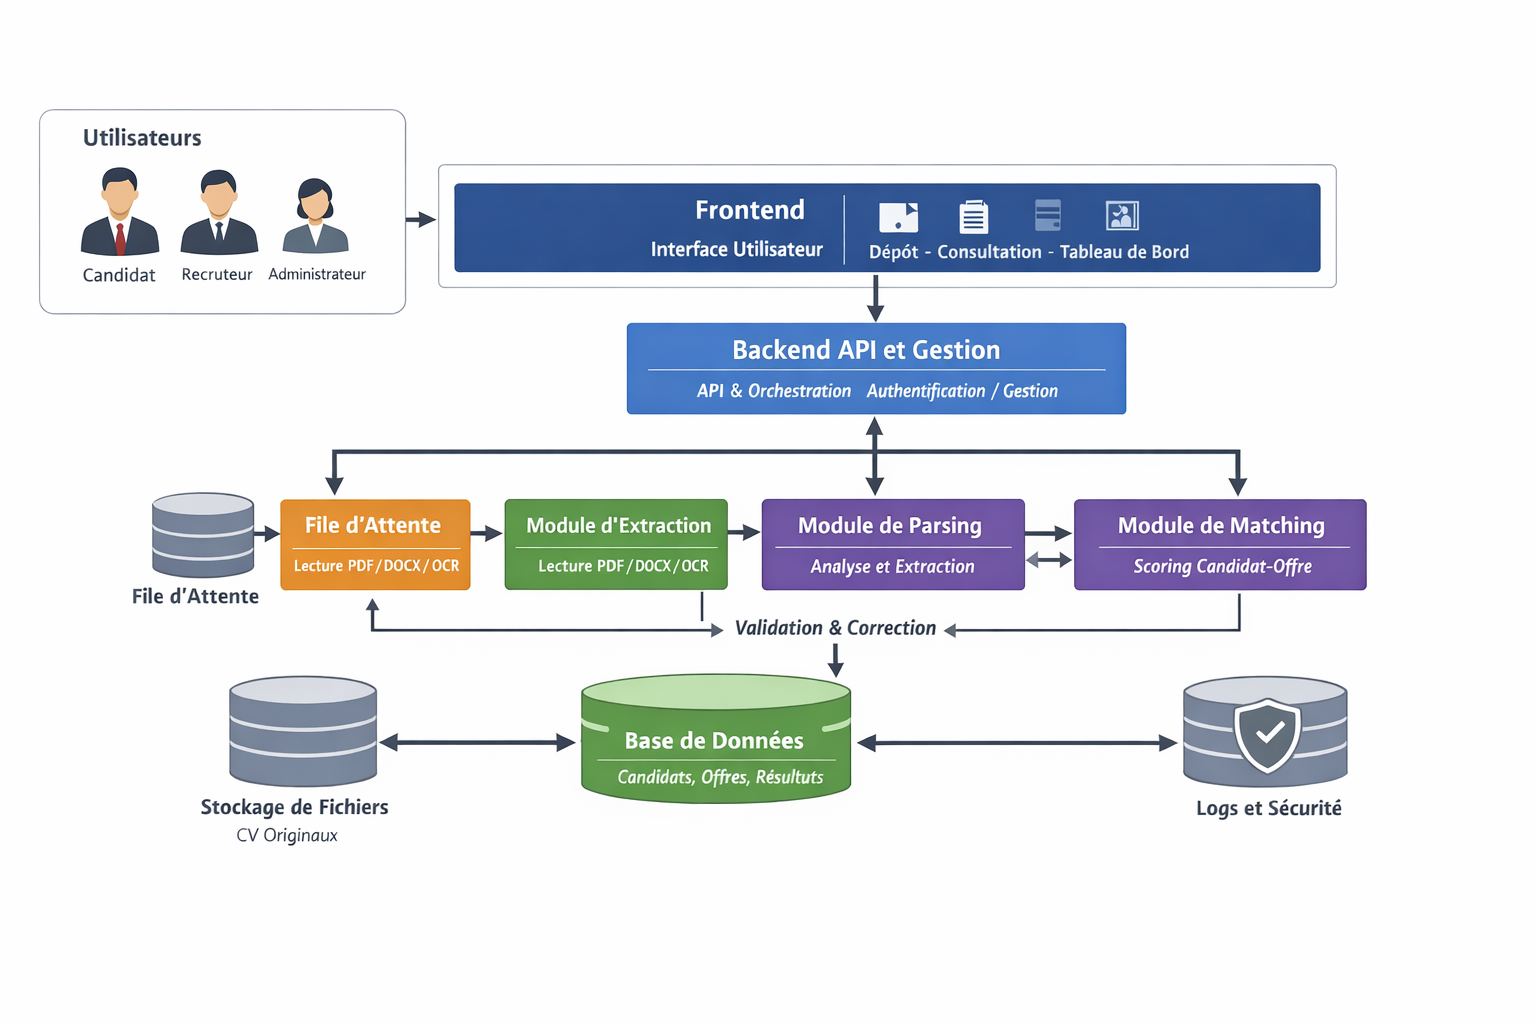
\includegraphics[width=0.95\textwidth]{architecture.png}
  \caption{Architecture globale de 3S TalentMatch}
  \label{fig:architecture}
\end{figure}

% ─────────────────────────────────────────────────────────────────────────────
\section{Workflow de traitement}

\subsection{Pipeline d'extraction des CV}

\begin{enumerate}
  \item L'utilisateur téléverse un CV via l'interface (PDF, DOCX ou image).
  \item Le module d'extraction sélectionne l'extracteur adapté au format (PDF textuel, DOCX, OCR).
  \item Le texte brut est transmis au pipeline NLP qui extrait les entités structurées.
  \item Les données structurées (\texttt{parsed\_data}) sont stockées dans la base de données.
\end{enumerate}

\subsection{Pipeline de matching candidat-offre}

\begin{enumerate}
  \item Le recruteur sélectionne une offre d'emploi.
  \item Le moteur de matching vectorise le profil candidat et le texte de l'offre via BGE-M3.
  \item Les scores TF-IDF, BERT (cross-encoder) et ML (MLP Fusion) sont calculés.
  \item Les scores sont fusionnés en un score final et les candidats sont classés.
  \item Les résultats avec explications sont affichés sur le dashboard RH.
\end{enumerate}

\subsection{Pipeline d'évaluation technique}

\begin{enumerate}
  \item Le recruteur sélectionne les candidats retenus après le matching et lance les évaluations (dates de passage et questions personnalisées optionnelles).
  \item Le modèle de langage local génère, une seule fois par offre et en arrière-plan, une réserve de questions ciblées sur les compétences requises (QCM à difficulté graduée et questions de raisonnement avec réponses de référence).
  \item Chaque candidat reçoit automatiquement une invitation par e-mail (lien personnel, code PIN à usage unique, dates) dès que son questionnaire est prêt ; chaque candidat reçoit un sous-ensemble de questions différent.
  \item Le candidat se connecte à son compte, saisit le PIN, accepte les règles, puis répond : QCM adaptatif (la difficulté s'ajuste à ses réponses) puis questions rédigées.
  \item Le système note les réponses localement (théorie de réponse à l'item pour les QCM, similarité sémantique BGE-M3 pour les rédactions), calcule l'écart entre compétences déclarées et démontrées, et trace les signaux d'intégrité.
  \item Le recruteur consulte les résultats : niveau par compétence, cohérence CV--test, rapport généré par IA et réponses détaillées.
\end{enumerate}

% ─────────────────────────────────────────────────────────────────────────────
\section{Diagrammes UML}

\subsection{Diagramme global des cas d'utilisation}

La figure~\ref{fig:usecase} présente le diagramme global des cas d'utilisation de la plateforme, structuré autour des trois acteurs identifiés. Le candidat gère son compte, dépose son CV (avec extraction et analyse automatiques) et consulte les offres ; le recruteur gère les offres, lance le matching candidat-offre, consulte les scores avec leurs explications et traite les candidatures ; l'administrateur gère les utilisateurs, les rôles et droits d'accès ainsi que les journaux d'accès.

\begin{figure}[H]
  \centering
  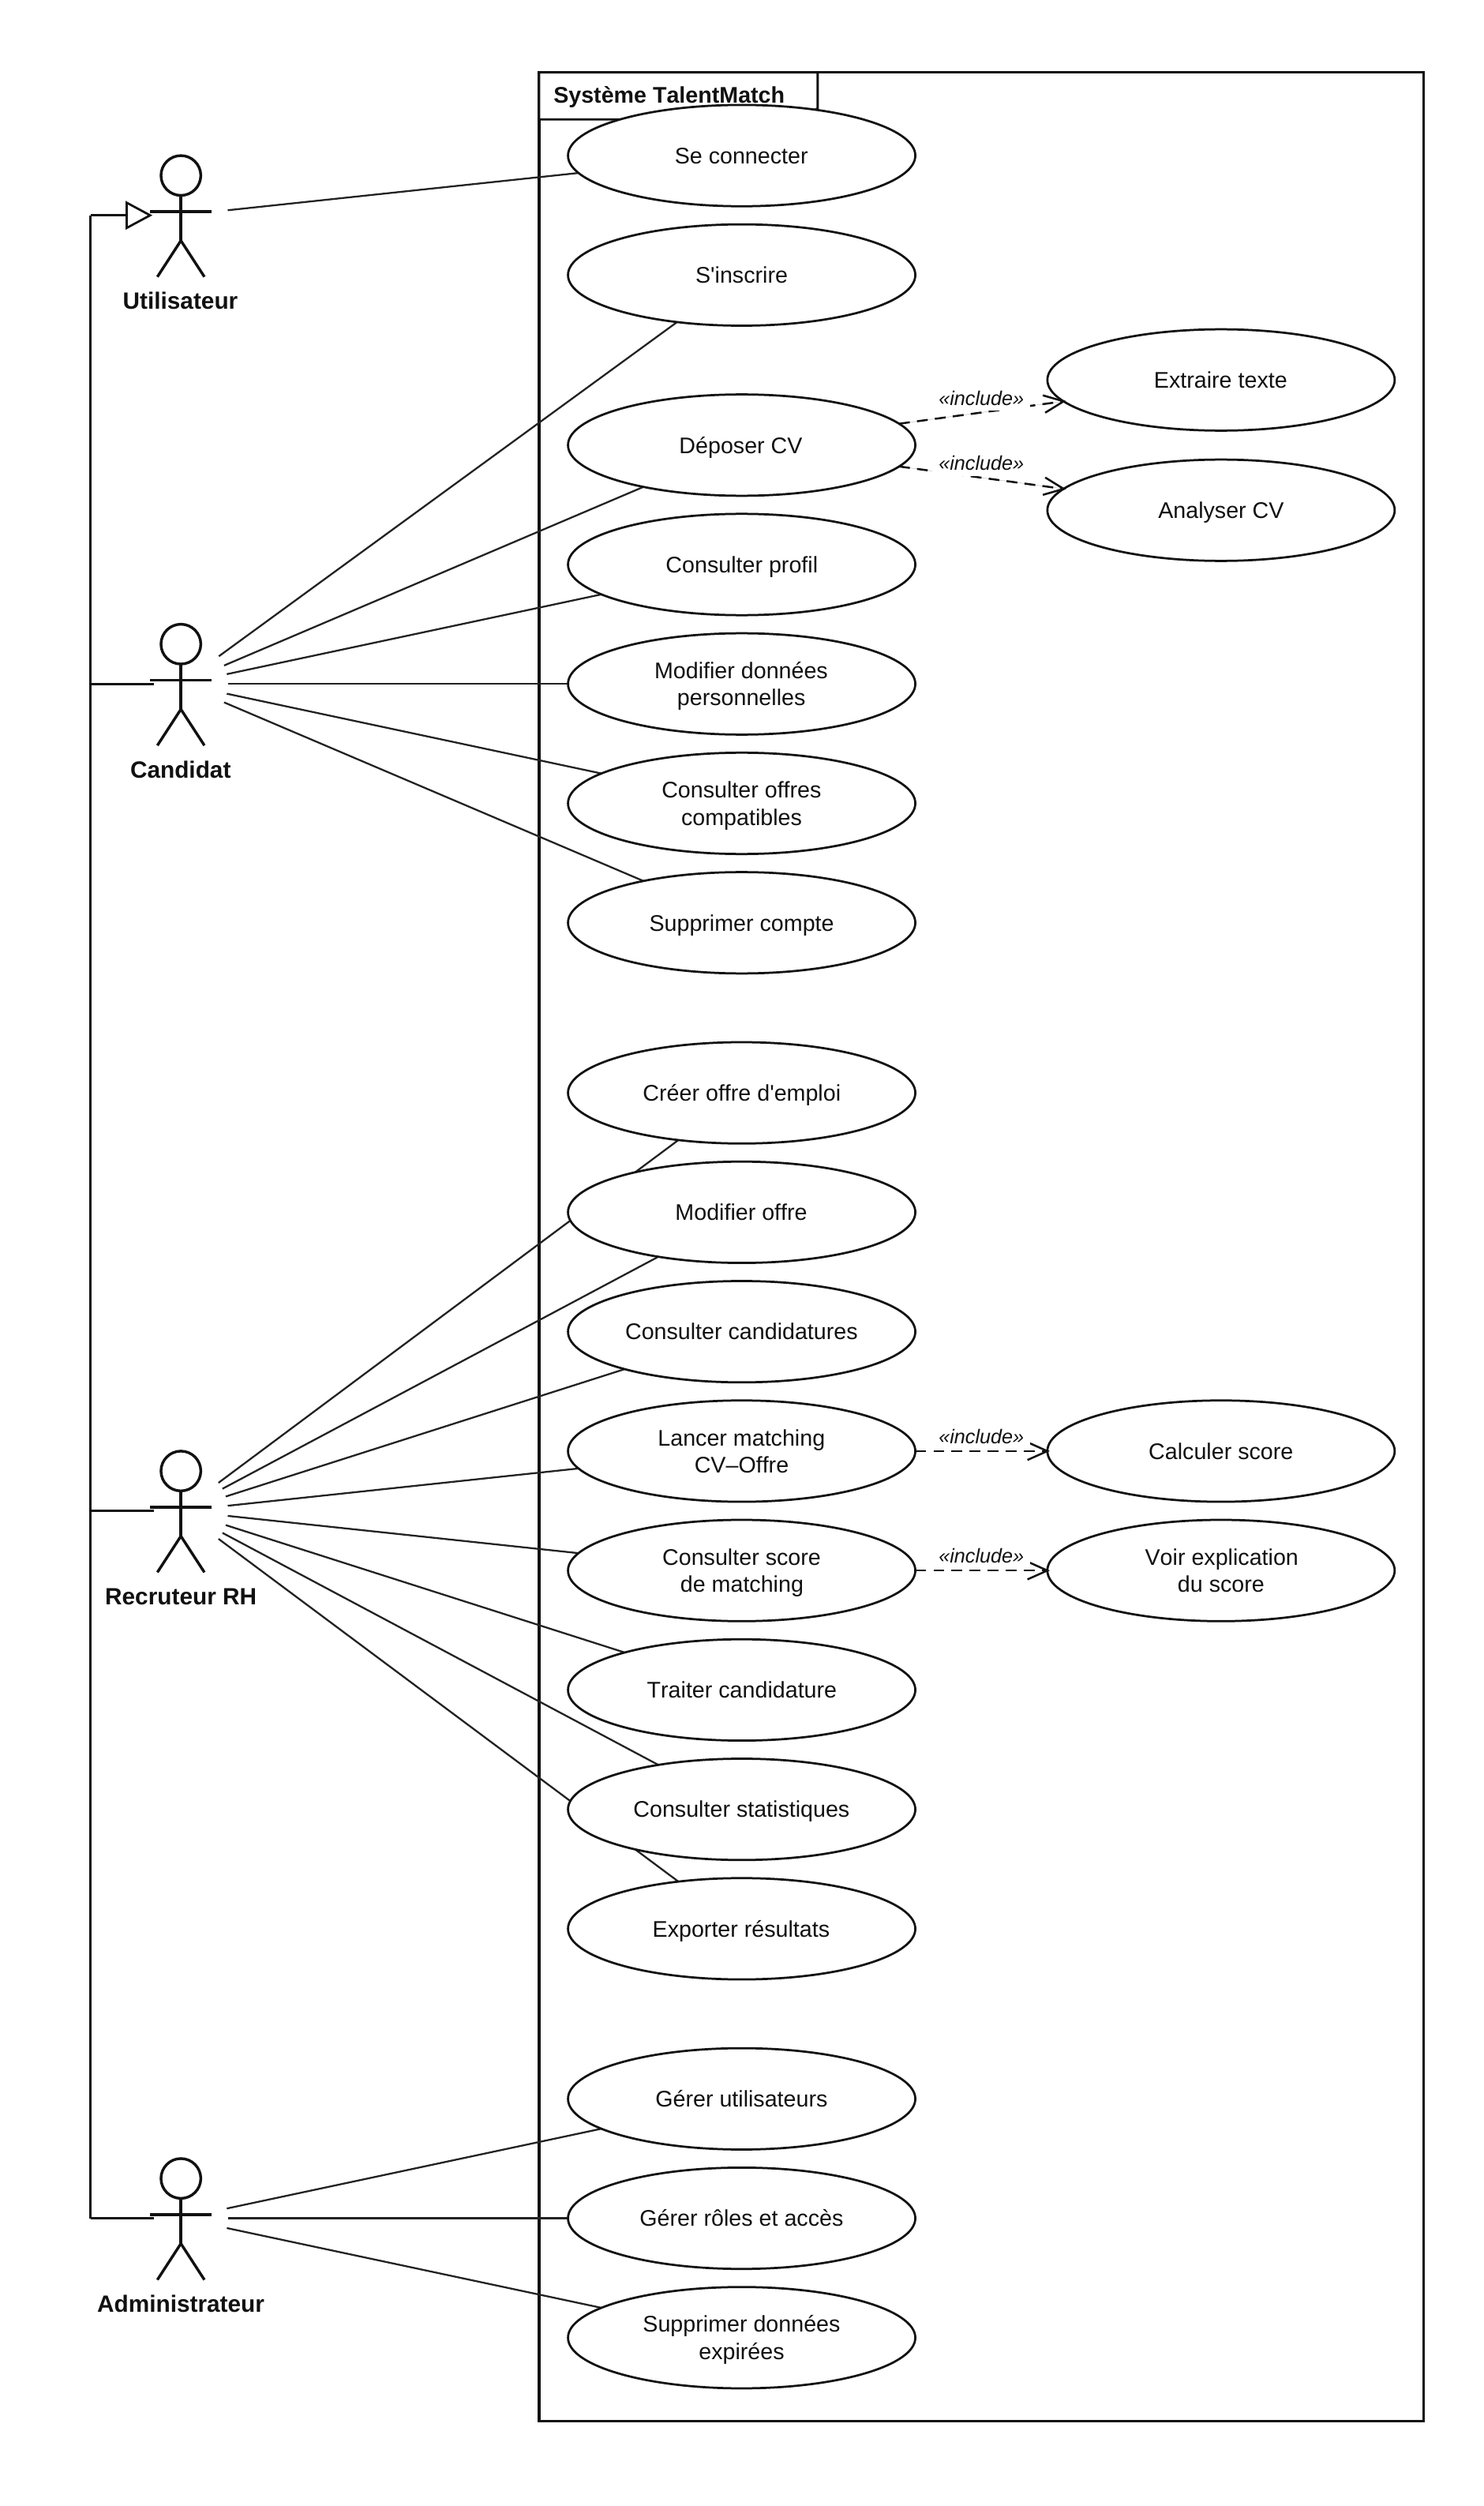
\includegraphics[width=0.95\textwidth]{diagrammecas-1.png}
  \caption{Diagramme global des cas d'utilisation}
  \label{fig:usecase}
\end{figure}

\subsection{Diagramme de séquence}

La figure~\ref{fig:sequence} illustre le flux principal de la plateforme, du téléversement d'un CV jusqu'à l'affichage des résultats de matching. Lors de l'extraction, l'API délègue l'extraction du texte au composant \texttt{CVExtractor}, qui choisit la méthode adaptée au format du fichier (pypdf pour les PDF textuels, python-docx pour les documents Word, EasyOCR pour les images et PDF scannés). Le texte brut est ensuite structuré par le \texttt{NLPParser}, qui enchaîne des extracteurs spécialisés (contact, entités, compétences, formations, expériences, langues) avant la persistance du profil en base. Lors du matching, le \texttt{MatchEngine} combine un score sémantique (BGE-M3) avec des scores de compétences, d'expérience et de formation pour produire un classement explicable des candidats.

\begin{figure}[H]
  \centering
  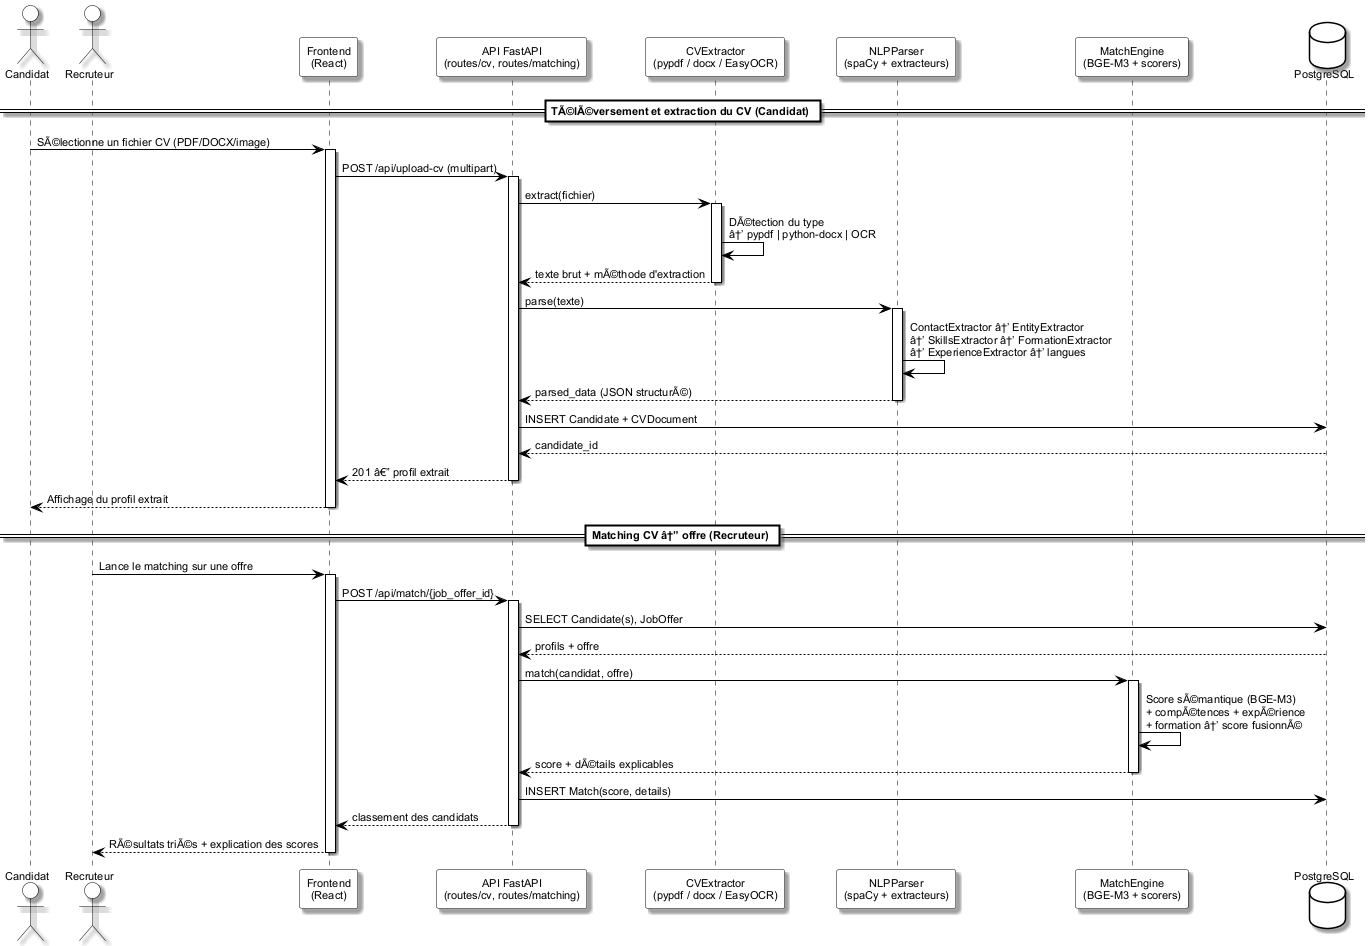
\includegraphics[width=\textwidth]{diagrams/diagramme_sequence.png}
  \caption{Diagramme de séquence — extraction d'un CV et matching candidat-offre}
  \label{fig:sequence}
\end{figure}

\subsection{Diagramme de classes global}

La figure~\ref{fig:classes} présente le diagramme de classes global de la plateforme, établi à partir du modèle de données réel. Il s'articule autour de quatre groupes : la gestion des utilisateurs et de la sécurité (\texttt{User}, \texttt{Notification}, \texttt{AccessLog}), le pipeline d'extraction des CV (\texttt{Candidate}, \texttt{CVDocument}), le matching (\texttt{JobOffer}, \texttt{Match}) et le module d'évaluation (\texttt{AssessmentSession}, \texttt{AssessmentQuestion}, \texttt{OpenQuestion}, \texttt{RealityGapResult}). Chaque candidat correspond à un profil extrait d'un CV ; une session d'évaluation relie un candidat à une offre et produit, à son terme, un résultat d'écart déclaré/démontré (\textit{Reality Gap}) qui vient ajuster le score de matching.

\begin{figure}[H]
  \centering
  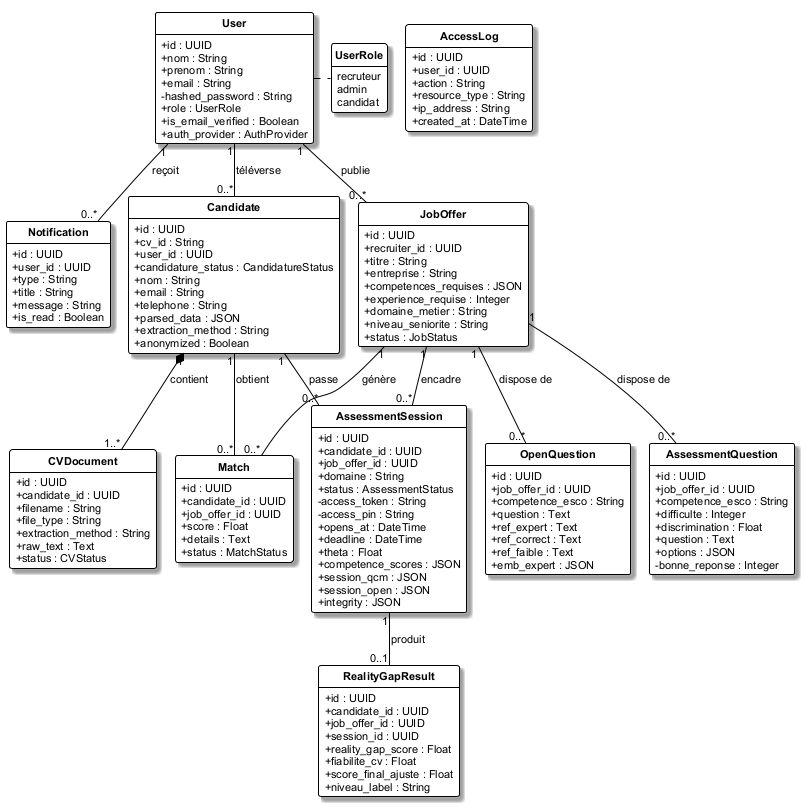
\includegraphics[width=\textwidth]{diagrams/diagramme_classes.png}
  \caption{Diagramme de classes global de la plateforme}
  \label{fig:classes}
\end{figure}

% ─────────────────────────────────────────────────────────────────────────────
\section{Backlog produit}

Le tableau~\ref{tab:backlog} présente le backlog produit de la plateforme 3S TalentMatch au format standard des user stories (\textit{En tant que\ldots, je veux\ldots, afin de\ldots}), avec le sprint de réalisation et la priorité de chaque story.

{\small
\setlength{\tabcolsep}{4pt}
\begin{longtable}{>{\bfseries}p{0.9cm} p{1.9cm} p{4.6cm} p{4.0cm} p{1.1cm} p{1.4cm}}
\caption{Backlog produit de 3S TalentMatch}
\label{tab:backlog} \\
\rowcolor{tabheader}
\textcolor{white}{\textbf{ID}} & \textcolor{white}{\textbf{En tant que\ldots}} & \textcolor{white}{\textbf{Je veux\ldots}} & \textcolor{white}{\textbf{Afin de\ldots}} & \textcolor{white}{\textbf{Sprint}} & \textcolor{white}{\textbf{Priorité}} \\
\endfirsthead
\multicolumn{6}{c}{\textit{(Suite du tableau~\ref{tab:backlog})}} \\
\rowcolor{tabheader}
\textcolor{white}{\textbf{ID}} & \textcolor{white}{\textbf{En tant que\ldots}} & \textcolor{white}{\textbf{Je veux\ldots}} & \textcolor{white}{\textbf{Afin de\ldots}} & \textcolor{white}{\textbf{Sprint}} & \textcolor{white}{\textbf{Priorité}} \\
\endhead
\midrule
\multicolumn{6}{r}{\textit{Suite page suivante}} \\
\endfoot
\bottomrule
\endlastfoot
US01 & Candidat & créer un compte et me connecter & accéder à mon espace personnel & 1 & Haute \\
\rowcolor{tabalt}
US02 & Candidat & me connecter via Google ou LinkedIn & m'inscrire sans créer de nouveau mot de passe & 1 & Moyenne \\
US03 & Admin & gérer les utilisateurs et les rôles & contrôler les accès à la plateforme & 1 & Haute \\
\rowcolor{tabalt}
US04 & Candidat & téléverser mon CV (PDF, DOCX, image) & postuler à une offre d'emploi & 2 & Haute \\
US05 & Système & extraire le texte du CV (dont OCR) & rendre tout document exploitable & 2 & Haute \\
\rowcolor{tabalt}
US06 & Système & structurer le texte en profil (parsing NLP) & alimenter le moteur de matching & 2 & Haute \\
US07 & Candidat & vérifier et corriger mes données extraites & garantir l'exactitude de mon profil & 2 & Moyenne \\
\rowcolor{tabalt}
US08 & Admin & créer les offres et y assigner des recruteurs & organiser le travail des équipes RH & 3 & Haute \\
US09 & RH & voir les candidats classés pour une offre & identifier rapidement les meilleurs profils & 3 & Haute \\
\rowcolor{tabalt}
US10 & RH & consulter le score de matching et son explication & justifier mes décisions de présélection & 3 & Haute \\
US11 & RH & consulter le dashboard de recrutement & suivre l'activité globale de recrutement & 3 & Haute \\
\rowcolor{tabalt}
US12 & RH & lancer les évaluations techniques (invitation e-mail, code PIN, dates) & vérifier les compétences des candidats retenus & 4 & Haute \\
US13 & Candidat & passer mon évaluation en ligne (QCM adaptatif, questions rédigées) & démontrer mes compétences réelles & 4 & Haute \\
\rowcolor{tabalt}
US14 & RH & consulter le rapport d'évaluation IA et la cohérence CV--test & prendre une décision éclairée & 4 & Haute \\
US15 & RH & disposer d'un score d'intégrité durant l'évaluation & détecter les comportements suspects & 4 & Moyenne \\
\rowcolor{tabalt}
US16 & Candidat & recevoir des notifications (e-mail et plateforme) & suivre l'avancement de ma candidature & 4 & Moyenne \\
US17 & Admin & consulter les journaux d'accès aux données & tracer l'accès aux données personnelles & 4 & Moyenne \\
\end{longtable}
}

% ─────────────────────────────────────────────────────────────────────────────
\section{Conclusion}

Ce chapitre a permis de définir les besoins fonctionnels et non fonctionnels du système 3S TalentMatch, de présenter l'architecture globale, le workflow de traitement et les diagrammes UML, ainsi que le backlog produit. Le chapitre suivant sera consacré à la réalisation des Sprints 1 et 2 : la mise en place du socle technique, de l'architecture backend et frontend et de l'authentification, puis la construction du pipeline d'extraction des CV (extraction, OCR, parsing NLP et stockage).

\newpage

% ═══════════════════════════════════════════════════════════════════════════════
%  CHAPITRES 3, 4, 5
% ═══════════════════════════════════════════════════════════════════════════════

\chapter{Sprints 1 et 2 : Socle technique et pipeline d'extraction des CV}

\section{Introduction}

Ce chapitre décrit la réalisation des deux premiers sprints du projet. Le Sprint~1 (semaines 3 à 6) est consacré à la mise en place des fondations : environnement de développement, architecture backend et frontend, base de données et système d'authentification multi-rôles. Le Sprint~2 (semaines 7 à 10) construit sur ce socle la première brique à valeur ajoutée de la plateforme : le pipeline d'extraction des CV, qui transforme un document brut (PDF, Word ou image scannée) en un profil candidat structuré et exploitable par le moteur de matching. Pour chaque sprint, nous présentons successivement la planification (objectif et backlog), la réalisation, les tests et la validation, la revue de sprint puis une conclusion.

% ═════════ SPRINT 1 ═════════
\section{Sprint 1 : Cadrage, conception et socle technique}

\subsection{Planification du sprint}

\subsubsection{Objectif du sprint}

L'objectif du Sprint~1 est de livrer un socle technique complet et opérationnel sur lequel l'ensemble des fonctionnalités métier pourront être construites. Concrètement, il s'agit de : mettre en place l'environnement de développement et l'outillage du projet ; définir et implémenter l'architecture du backend (API REST) et du frontend (application web monopage) ; créer la base de données et son mécanisme de migrations ; et livrer un système d'authentification sécurisé gérant les trois rôles de la plateforme (candidat, recruteur, administrateur).

\subsubsection{Backlog du sprint}

Le tableau~\ref{tab:backlog-s1} présente les user stories retenues pour ce sprint, extraites du backlog produit (tableau~\ref{tab:backlog}), et le tableau~\ref{tab:taches-s1} leur découpage en tâches techniques.

\begin{table}[H]
\centering
\caption{User stories du Sprint 1}
\label{tab:backlog-s1}
\small
\begin{tabularx}{\textwidth}{>{\bfseries}p{0.9cm} p{1.9cm} X X p{1.4cm}}
\rowcolor{tabheader}
\textcolor{white}{\textbf{ID}} & \textcolor{white}{\textbf{En tant que\ldots}} & \textcolor{white}{\textbf{Je veux\ldots}} & \textcolor{white}{\textbf{Afin de\ldots}} & \textcolor{white}{\textbf{Priorité}} \\
US01 & Candidat & créer un compte et me connecter & accéder à mon espace personnel & Haute \\
\rowcolor{tabalt}
US02 & Candidat & me connecter via Google ou LinkedIn & m'inscrire sans créer de nouveau mot de passe & Moyenne \\
US03 & Admin & gérer les utilisateurs et les rôles & contrôler les accès à la plateforme & Haute \\
\bottomrule
\end{tabularx}
\end{table}

\begin{table}[H]
\centering
\caption{Découpage en tâches techniques du Sprint 1}
\label{tab:taches-s1}
\small
\begin{tabularx}{\textwidth}{>{\bfseries}p{1.2cm} X}
\rowcolor{tabheader}
\textcolor{white}{\textbf{US}} & \textcolor{white}{\textbf{Tâches techniques}} \\
US01 & Modèle \texttt{User} ; inscription avec vérification par code e-mail (OTP) ; connexion JWT ; réinitialisation du mot de passe. \\
\rowcolor{tabalt}
US02 & Intégration OAuth~2.0 (Google, LinkedIn) ; création automatique du compte au premier accès. \\
US03 & Rôles \texttt{candidat} / \texttt{recruteur} / \texttt{admin} ; interface d'administration ; activation/désactivation des comptes. \\
\rowcolor{tabalt}
--- & \textit{Tâches transverses} : arborescence backend FastAPI ; base PostgreSQL et migrations Alembic ; squelette frontend React ; client HTTP centralisé ; routage protégé. \\
\bottomrule
\end{tabularx}
\end{table}

\subsection{Réalisation du sprint}

\subsubsection{Environnement de travail et outils}

L'environnement de développement retenu est résumé dans le tableau~\ref{tab:outils-s1}. Les choix ont été guidés par les standards de l'entreprise et par la contrainte de traitement 100\,\% local des données (aucun service externe n'intervient dans le traitement des CV).

\begin{table}[H]
\centering
\caption{Outils et technologies mis en place au Sprint 1}
\label{tab:outils-s1}
\begin{tabularx}{\textwidth}{lX}
\toprule
\textbf{Catégorie} & \textbf{Outils} \\
\midrule
Langages & Python 3.10 (backend), JavaScript ES2022 (frontend) \\
Backend & FastAPI, SQLAlchemy~2, Alembic, Uvicorn \\
Frontend & React 18, Vite 5, React Router 6, Axios, Tailwind CSS \\
Base de données & PostgreSQL 16 \\
Gestion de versions & Git, GitHub (branches par fonctionnalité) \\
Tests \& documentation API & pytest, Swagger UI (généré automatiquement par FastAPI) \\
Environnement & Visual Studio Code, environnements virtuels Python (venv) \\
\bottomrule
\end{tabularx}
\end{table}

\subsubsection{Architecture backend (FastAPI)}

Le backend est une API REST développée avec FastAPI, choisie pour ses performances, sa validation automatique des données (Pydantic) et sa documentation interactive générée automatiquement (Swagger). L'arborescence adoptée sépare strictement les responsabilités :

\begin{itemize}
  \item \texttt{app/routes/} --- un module par ressource (authentification, CV, offres, matching, administration, notifications) exposant les endpoints HTTP ;
  \item \texttt{app/services/} --- la logique métier (services d'authentification, d'e-mail, d'extraction, de NLP, de matching), indépendante de la couche HTTP ;
  \item \texttt{app/models/} --- les entités SQLAlchemy correspondant au diagramme de classes de la figure~\ref{fig:classes} ;
  \item \texttt{app/schemas/} --- les DTO Pydantic qui valident les entrées et sérialisent les sorties de l'API.
\end{itemize}

La persistance repose sur PostgreSQL. Le schéma de la base est versionné par des migrations Alembic : chaque évolution du modèle de données donne lieu à une migration rejouable, ce qui garantit la reproductibilité de la base sur tout environnement (développement, production).

\subsubsection{Architecture frontend (React)}

Le frontend est une application monopage (SPA) React~18, construite avec Vite. Deux choix structurants méritent d'être soulignés :

\begin{itemize}
  \item \textbf{Client HTTP centralisé} : toutes les requêtes passent par une instance Axios unique qui injecte automatiquement le jeton JWT dans les en-têtes, et qui intercepte les réponses \texttt{401} pour déconnecter l'utilisateur et le rediriger vers la page de connexion. Cette centralisation fait de la gestion de session un invariant de l'application ;
  \item \textbf{Routage protégé} : un composant \texttt{ProtectedRoute} vérifie l'authentification et le rôle de l'utilisateur avant de rendre chaque page sensible, ce qui empêche tout accès direct par URL à une page non autorisée.
\end{itemize}

En développement, le serveur Vite fait office de proxy vers l'API (\texttt{/api/*} $\rightarrow$ backend), ce qui évite les problèmes de partage de ressources entre origines (CORS).

\subsubsection{Authentification et gestion des rôles}

Le système d'authentification est la brique de sécurité centrale de la plateforme. Quatre parcours ont été implémentés.

\paragraph{Inscription avec vérification e-mail.} À la création du compte, l'adresse e-mail est validée par un code à usage unique (OTP) à durée de validité limitée, envoyé par e-mail : le compte n'est activé qu'après saisie du bon code. Ce mécanisme garantit que chaque compte correspond à une adresse réellement contrôlée par son titulaire --- prérequis indispensable puisque les invitations aux évaluations et les codes PIN transiteront par ce canal. Le mot de passe choisi n'est jamais stocké en clair : il est haché avec l'algorithme \textbf{bcrypt} (bibliothèque \texttt{passlib}), un algorithme adaptatif volontairement lent et salé, résistant aux attaques par force brute et par tables précalculées.

\paragraph{Connexion et session.} Après vérification des identifiants, le backend délivre un \textbf{jeton JWT signé} (bibliothèque \texttt{python-jose}) contenant l'identité et le rôle de l'utilisateur, avec une durée de validité limitée. Ce jeton est présenté à chaque requête (schéma \textit{Bearer}) ; le backend vérifie systématiquement sa signature et son expiration. L'API étant ainsi \textit{sans état}, aucune session serveur n'est à maintenir, ce qui simplifie la montée en charge.

\paragraph{Connexion OAuth 2.0.} En alternative, l'utilisateur peut se connecter via un compte Google ou LinkedIn : le frontend obtient un jeton d'identité auprès du fournisseur, le backend en vérifie la signature auprès de ce fournisseur, extrait l'adresse e-mail vérifiée et crée automatiquement le compte local au premier accès (champ \texttt{auth\_provider}, sans mot de passe local). L'utilisateur bénéficie ainsi d'une inscription sans friction, l'e-mail étant déjà vérifié par le fournisseur d'identité.

\paragraph{Réinitialisation du mot de passe.} Un parcours « mot de passe oublié » complète le dispositif : un code à durée limitée est envoyé par e-mail et permet de définir un nouveau mot de passe, sans jamais révéler l'ancien (qui n'est de toute façon pas récupérable, seul son hachage étant stocké).

Enfin, la plateforme distingue \textbf{trois rôles} --- \texttt{candidat}, \texttt{recruteur}, \texttt{admin} --- conformément à la matrice des permissions du tableau~\ref{tab:matrice-roles} : chaque endpoint sensible vérifie le rôle porté par le jeton avant de servir la requête, et retourne \texttt{403} en cas de droits insuffisants.

La figure~\ref{fig:connexion} présente la page de connexion de la plateforme (connexion classique et via Google/LinkedIn), et la figure~\ref{fig:inscription} la page d'inscription.

\begin{figure}[H]
  \centering
  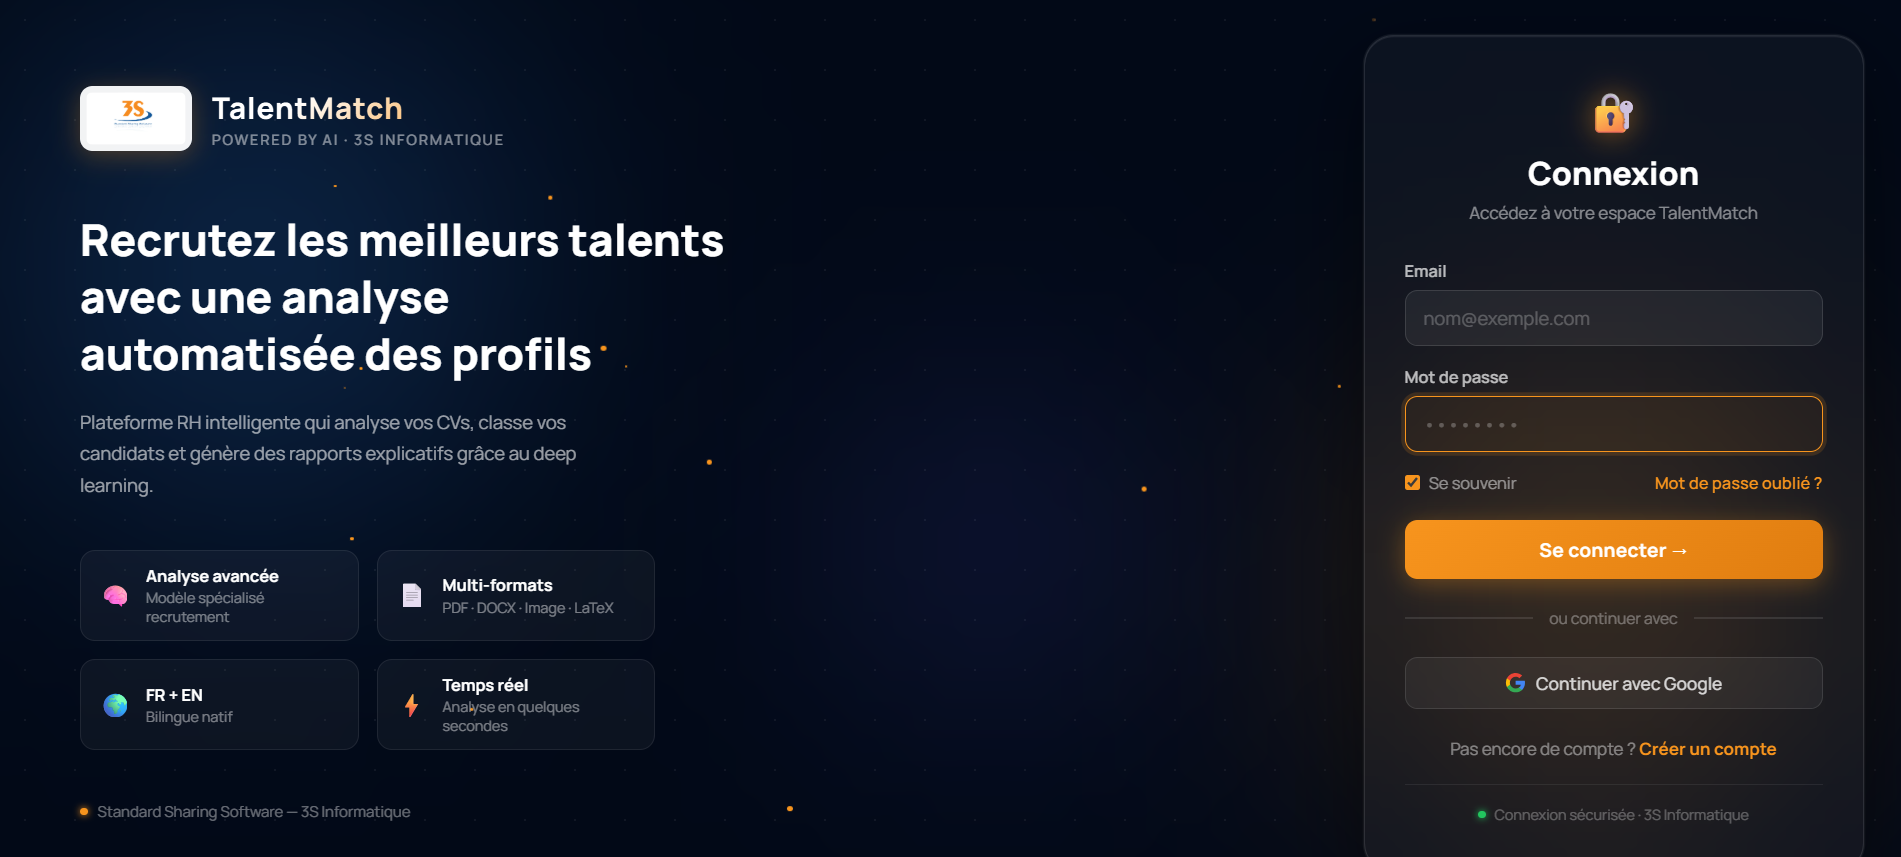
\includegraphics[width=0.85\textwidth]{captures/connexion.png}
  \caption{Page de connexion de la plateforme}
  \label{fig:connexion}
\end{figure}

\begin{figure}[H]
  \centering
  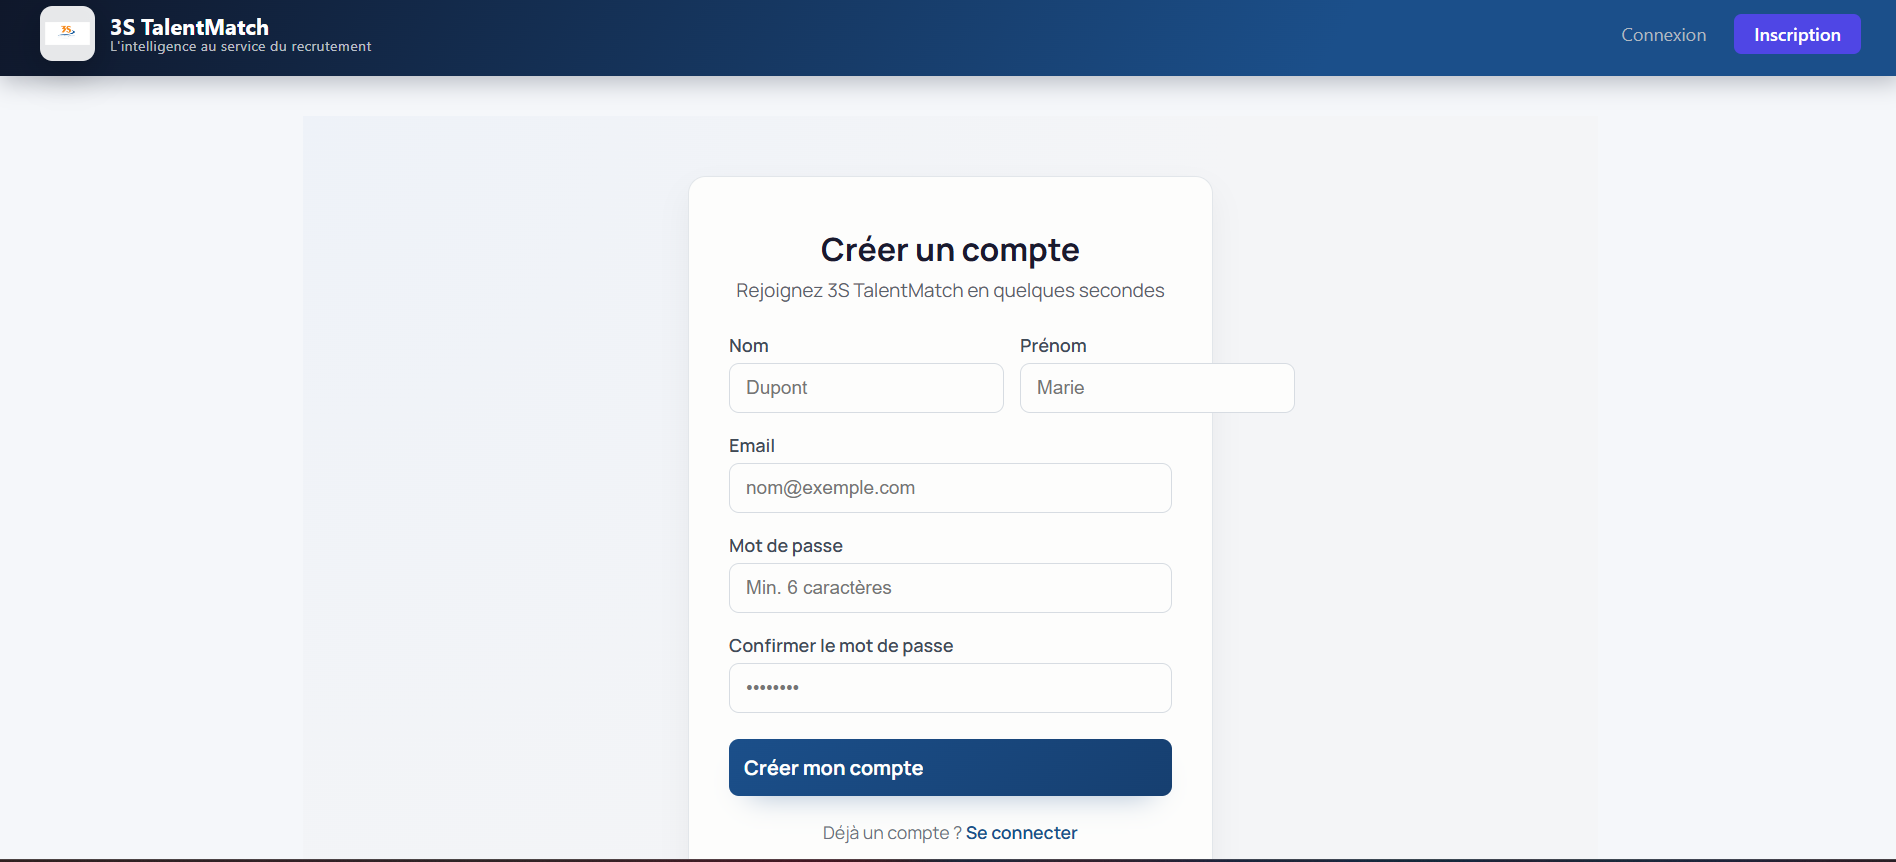
\includegraphics[width=0.85\textwidth]{captures/inscription.png}
  \caption{Page d'inscription}
  \label{fig:inscription}
\end{figure}

La figure~\ref{fig:otp} illustre la vérification e-mail : après l'inscription, le candidat saisit le code à six chiffres reçu par e-mail. Le compte n'est activé qu'après validation de ce code dans la fenêtre de validité définie côté serveur.

\begin{figure}[H]
  \centering
  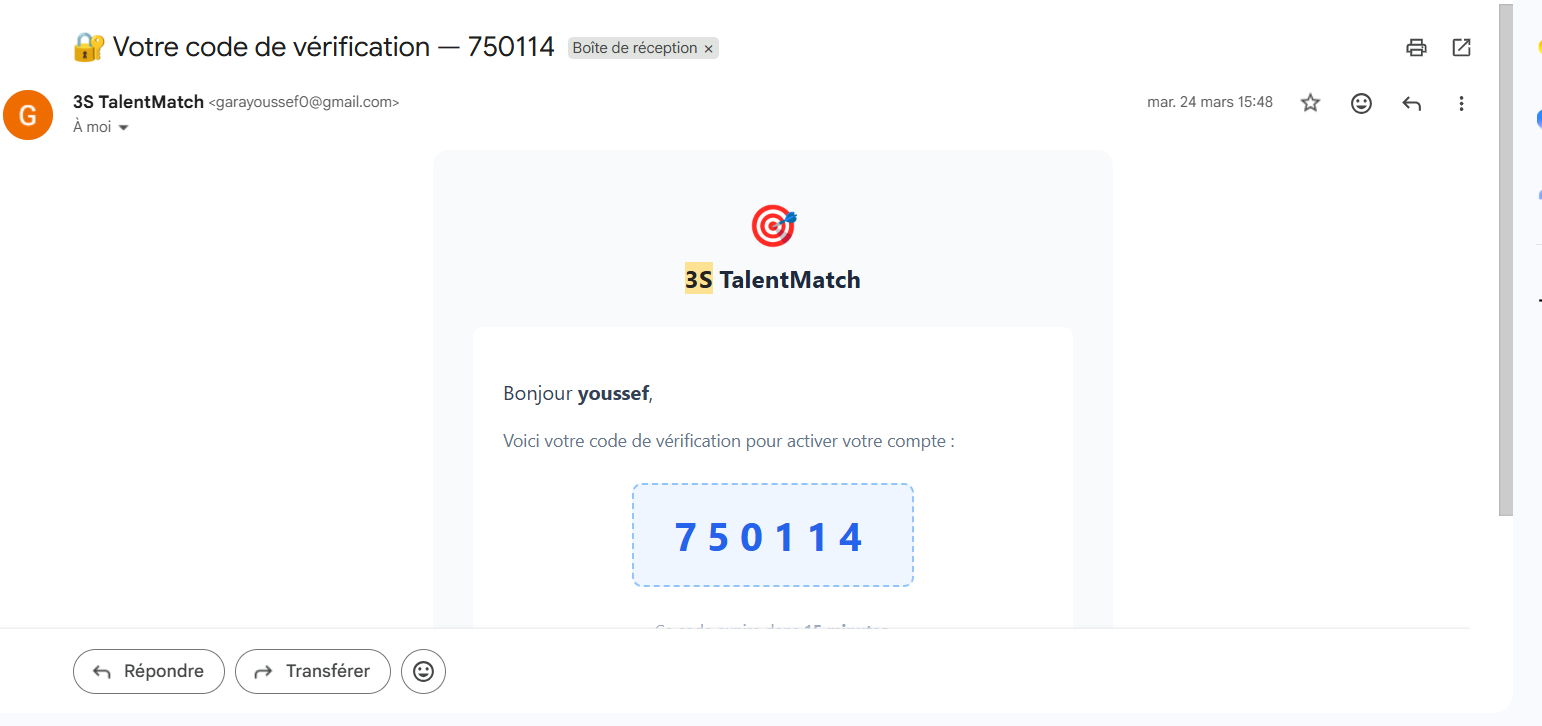
\includegraphics[width=0.75\textwidth]{captures/verification_otp.png}
  \caption{Vérification de l'adresse e-mail par code OTP à l'inscription}
  \label{fig:otp}
\end{figure}

\subsection{Tests et validation du sprint}

La validation du sprint a combiné tests automatisés et scénarios manuels :

\begin{itemize}
  \item \textbf{Tests unitaires} (pytest) sur le service d'authentification : hachage et vérification des mots de passe, génération et décodage des JWT, expiration des codes OTP ;
  \item \textbf{Scénarios de bout en bout} via Swagger et le frontend : inscription $\rightarrow$ réception du code $\rightarrow$ activation $\rightarrow$ connexion $\rightarrow$ accès à une ressource protégée ; tentative d'accès sans jeton ou avec un jeton expiré (rejet \texttt{401} attendu) ; tentative d'accès à une ressource d'administration avec un compte candidat (rejet \texttt{403} attendu) ;
  \item \textbf{Connexions OAuth} testées avec des comptes Google et LinkedIn réels.
\end{itemize}

L'ensemble des scénarios prévus ont été validés à la fin du sprint.

\subsection{Revue du sprint}

La revue de sprint, menée avec l'encadrant en entreprise, a permis de valider le socle livré : architecture claire, authentification fonctionnelle pour les trois rôles, base de données migrée et documentée. La principale remarque a porté sur la nécessité de préparer dès ce stade la journalisation des accès aux données personnelles (finalement implémentée au Sprint~4 avec la table \texttt{access\_logs}), les CV traités par la suite contenant des données sensibles.

\subsection{Conclusion du sprint}

Le Sprint~1 a livré l'intégralité de son périmètre : un backend FastAPI structuré et migré, un frontend React sécurisé et un système d'authentification multi-rôles complet. Ces fondations permettent d'aborder le Sprint~2 --- le pipeline d'extraction des CV --- en concentrant l'effort sur la valeur métier, l'infrastructure étant désormais stable.

% ═════════ SPRINT 2 ═════════
\section{Sprint 2 : Extraction, parsing et structuration des CV}

\subsection{Planification du sprint}

\subsubsection{Objectif du sprint}

L'objectif du Sprint~2 est de livrer le pipeline complet d'extraction des CV : un candidat téléverse son CV dans n'importe quel format courant (PDF textuel, PDF scanné, document Word, image), et le système en extrait automatiquement un profil structuré --- identité, contact, compétences, expériences, formations, langues --- prêt à être exploité par le moteur de matching. Ce sprint constitue la première brique d'intelligence artificielle de la plateforme.

\subsubsection{Backlog du sprint}

Le tableau~\ref{tab:backlog-s2} présente les user stories du sprint, et le tableau~\ref{tab:taches-s2} leur découpage en tâches techniques.

\begin{table}[H]
\centering
\caption{User stories du Sprint 2}
\label{tab:backlog-s2}
\small
\begin{tabularx}{\textwidth}{>{\bfseries}p{0.9cm} p{1.9cm} X X p{1.4cm}}
\rowcolor{tabheader}
\textcolor{white}{\textbf{ID}} & \textcolor{white}{\textbf{En tant que\ldots}} & \textcolor{white}{\textbf{Je veux\ldots}} & \textcolor{white}{\textbf{Afin de\ldots}} & \textcolor{white}{\textbf{Priorité}} \\
US04 & Candidat & téléverser mon CV (PDF, DOCX, image) & postuler à une offre d'emploi & Haute \\
\rowcolor{tabalt}
US05 & Système & extraire le texte du CV (dont OCR) & rendre tout document exploitable & Haute \\
US06 & Système & structurer le texte en profil (parsing NLP) & alimenter le moteur de matching & Haute \\
\rowcolor{tabalt}
US07 & Candidat & vérifier et corriger mes données extraites & garantir l'exactitude de mon profil & Moyenne \\
\bottomrule
\end{tabularx}
\end{table}

\begin{table}[H]
\centering
\caption{Découpage en tâches techniques du Sprint 2}
\label{tab:taches-s2}
\small
\begin{tabularx}{\textwidth}{>{\bfseries}p{1.2cm} X}
\rowcolor{tabheader}
\textcolor{white}{\textbf{US}} & \textcolor{white}{\textbf{Tâches techniques}} \\
US04 & Endpoint de téléversement ; contrôle du type et de la taille du fichier ; interface de dépôt depuis la page d'une offre. \\
\rowcolor{tabalt}
US05 & Extracteur unifié avec détection du format ; extraction PDF (PyMuPDF/pypdf) ; Word (python-docx) ; OCR des documents scannés (EasyOCR) ; détection automatique des PDF sans couche texte ; cache OCR. \\
US06 & Pipeline NLP : détection de sections ; extracteurs spécialisés (contact, entités, compétences, formations, expériences, langues) ; modèle spaCy français ; normalisation ESCO. \\
\rowcolor{tabalt}
US07 & Affichage du profil extrait ; édition des champs avant validation. \\
\bottomrule
\end{tabularx}
\end{table}

\subsection{Réalisation du sprint}

\subsubsection{Module d'extraction multi-formats (PDF, DOCX, OCR)}

Le composant \texttt{CVExtractor} constitue le point d'entrée unique de l'extraction : il détecte le format du fichier et délègue au sous-extracteur approprié.

\begin{itemize}
  \item \textbf{PDF textuel} : l'extraction privilégie PyMuPDF, qui fournit la position de chaque bloc de texte ; cette information permet de reconstruire l'ordre de lecture des CV en colonnes (mise en page très fréquente), là où une extraction naïve mélangerait les colonnes. La bibliothèque pypdf est conservée en solution de repli ;
  \item \textbf{Document Word} : extraction directe des paragraphes et tableaux via python-docx ;
  \item \textbf{PDF scanné et image} : lorsque le PDF ne contient pas de couche texte (détection automatique par densité de texte extrait), le document est converti en images et traité par reconnaissance optique de caractères (OCR) avec EasyOCR. Un cache des résultats OCR évite de retraiter un même document, l'OCR étant l'étape la plus coûteuse du pipeline.
\end{itemize}

Chaque extraction retourne, en plus du texte, des métadonnées de provenance (méthode utilisée, nombre de pages, recours ou non à l'OCR) qui sont conservées tout au long du pipeline à des fins de traçabilité et de diagnostic.

\subsubsection{Pipeline NLP et parsing}

Le texte brut est ensuite transformé en données structurées par le composant \texttt{NLPParser}, qui orchestre une chaîne d'extracteurs spécialisés. Chaque extracteur est une classe indépendante avec un point d'entrée unique \texttt{extract()}, ce qui permet de les tester unitairement et de les faire évoluer séparément.

\paragraph{Détection de sections.} Avant toute extraction, le texte est segmenté en sections logiques (expériences, formation, compétences, langues, certifications\ldots) à l'aide d'un dictionnaire de motifs d'intitulés couvrant les variantes françaises et anglaises (« Expérience professionnelle », « Work Experience », « Parcours »\ldots). Cette segmentation permet aux extracteurs suivants de travailler sur la bonne portion du document et évite les confusions --- par exemple, une technologie citée dans un intitulé de formation ne doit pas être comptée comme une expérience.

\paragraph{Extraction des contacts.} L'e-mail, le téléphone et les liens de profils (LinkedIn, GitHub, site personnel) sont extraits par expressions régulières robustes. Les numéros de téléphone gèrent les formats tunisiens et internationaux (indicatifs, séparateurs variables, numéros collés au texte par l'OCR). En présence de plusieurs candidats possibles (ex. : deux e-mails), une heuristique de priorité choisit la valeur principale, les autres restant disponibles dans le profil.

\paragraph{Identification du candidat.} Le nom est identifié par la reconnaissance d'entités nommées du modèle spaCy français \texttt{fr\_core\_news\_md} (entités de type personne), croisée avec des heuristiques de position et de mise en forme : le nom figure généralement dans les premières lignes, souvent en capitales ou détaché du corps du texte. Cette combinaison statistique + heuristique s'est révélée nettement plus fiable que chaque approche isolée sur les mises en page variées du corpus. La provenance de chaque champ (quel extracteur l'a produit, avec quelle confiance) est conservée dans les métadonnées du profil.

\paragraph{Extraction des compétences.} Les compétences sont détectées par correspondance avec le référentiel européen \textbf{ESCO} (plusieurs milliers de compétences normalisées, avec variantes et synonymes multilingues), complété par des listes de technologies courantes. Chaque compétence détectée est \textbf{normalisée} vers sa forme canonique --- « ReactJS », « React.js » et « React » deviennent la même entrée --- et classée par catégorie (développement web, cloud, données, méthodologies\ldots). Cette normalisation est la condition du matching du Sprint~3 : sans elle, le moteur comparerait des chaînes de caractères au lieu de comparer des concepts.

\paragraph{Formations et expériences.} L'extracteur de formations identifie les diplômes, établissements et années, et en déduit une estimation du \textbf{niveau d'études} (Bac+2 à Bac+8) utilisée par le matching pour la comparaison avec le niveau requis par l'offre. L'extracteur d'expériences reconstitue les postes occupés (intitulé, entreprise, période) et calcule la \textbf{durée totale d'expérience professionnelle}, en gérant les périodes qui se chevauchent et les postes en cours (« depuis 2023 »).

\paragraph{Langues.} Les langues déclarées et leur niveau (courant, intermédiaire, notions, ou cadre européen A1--C2) complètent le profil.

\paragraph{Robustesse et diagnostic.} Le pipeline est conçu pour dégrader proprement : si le modèle spaCy n'est pas disponible, le système bascule sur un traitement de repli et l'enregistre dans les métadonnées du profil (\texttt{spacy\_fallback}) ; un endpoint de diagnostic (\texttt{/api/nlp/status}) expose à tout moment l'état des composants NLP (modèles chargés, versions, options actives), ce qui facilite l'exploitation et le support.

\subsubsection{Structuration des données et stockage en base}

Le résultat du parsing est un document JSON normalisé (schéma Pydantic \texttt{cv\_data}) regroupant l'ensemble des informations extraites et leurs métadonnées de provenance. Il est persisté dans l'entité \texttt{Candidate} (champ \texttt{parsed\_data}), tandis que le fichier d'origine et son texte brut sont tracés dans l'entité \texttt{CVDocument} avec leur statut de traitement (\texttt{uploaded}, \texttt{extracted}, \texttt{parsed}, \texttt{error}). Ce choix d'un stockage JSON flexible permet d'enrichir le schéma d'extraction sans migration de base à chaque évolution.

\subsubsection{Interface de téléversement}

Côté frontend, le candidat dépose son CV directement depuis la page d'une offre d'emploi (figure~\ref{fig:upload}) : le formulaire de candidature accepte les formats PDF, DOCX et image, et affiche une mention d'information sur l'utilisation des données personnelles avant le dépôt. Une fois le pipeline exécuté, le profil extrait est affiché pour vérification (figure~\ref{fig:profil}) : identité, contact, compétences groupées par catégorie, expériences, formations et langues, accompagnés des métadonnées de traitement (méthode d'extraction, indice de confiance du parsing). Le candidat comme le recruteur peuvent ainsi contrôler la sortie du pipeline automatique (US07), ce qui introduit une supervision humaine permanente.

\begin{figure}[H]
  \centering
  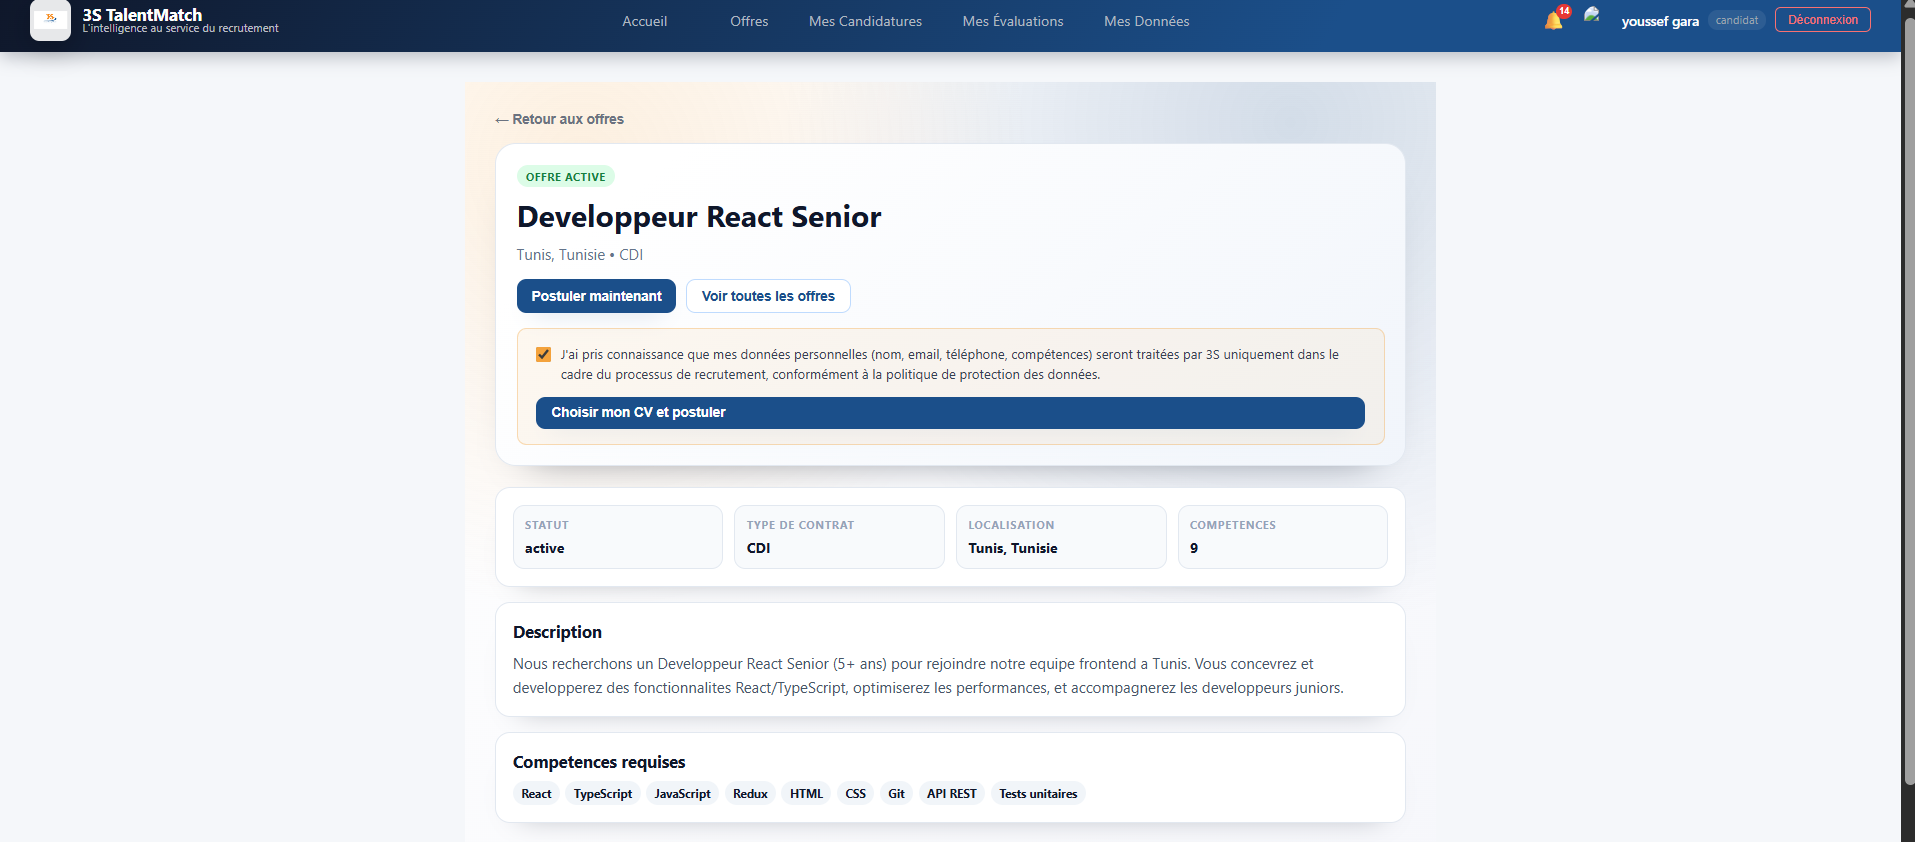
\includegraphics[width=0.85\textwidth]{captures/upload_cv.png}
  \caption{Candidature à une offre : dépôt du CV avec mention d'information sur les données personnelles}
  \label{fig:upload}
\end{figure}

\begin{figure}[H]
  \centering
  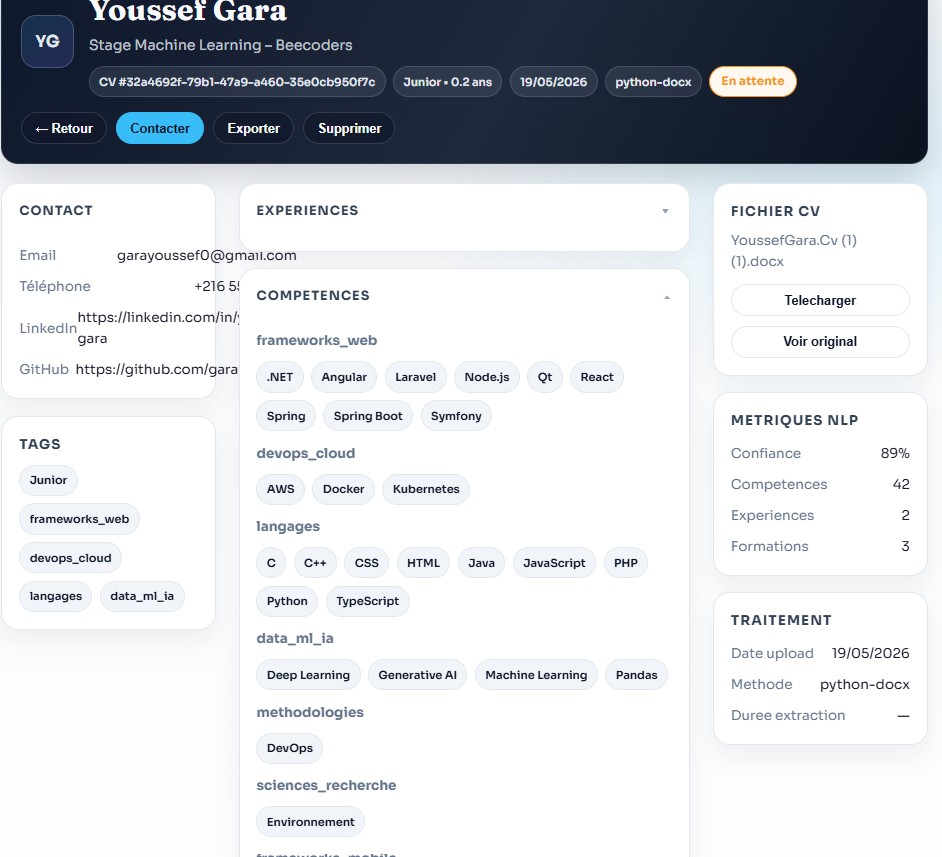
\includegraphics[width=0.85\textwidth]{captures/profil_extrait.png}
  \caption{Profil candidat structuré, extrait automatiquement du CV (compétences par catégorie, métriques NLP et traçabilité du traitement)}
  \label{fig:profil}
\end{figure}

\subsection{Tests et validation du sprint}

Outre les tests unitaires des extracteurs (pytest), le pipeline complet a été validé par un traitement par lot sur un corpus de \textbf{90 CV réels} de profils et de domaines variés (informatique, finance, marketing, juridique, santé), couvrant les trois familles de formats supportées : 77 PDF, 9 images scannées (JPG/PNG) et 4 documents Word. Chaque CV a traversé la chaîne complète extraction $\rightarrow$ parsing NLP, et les sorties ont été mesurées automatiquement. Le tableau~\ref{tab:metriques-s2} synthétise les résultats.

\begin{table}[H]
\centering
\caption{Résultats de la validation du pipeline d'extraction sur 90 CV réels}
\label{tab:metriques-s2}
\small
\begin{tabularx}{\textwidth}{X r}
\rowcolor{tabheader}
\textcolor{white}{\textbf{Indicateur}} & \textcolor{white}{\textbf{Résultat}} \\
Taux d'extraction du texte (tous formats) & \textbf{100\,\%} (90/90) \\
\rowcolor{tabalt}
\quad dont PDF (PyMuPDF/pypdf) & 100\,\% (77/77) \\
\quad dont images scannées (OCR EasyOCR) & 100\,\% (9/9) \\
\rowcolor{tabalt}
\quad dont documents Word (python-docx) & 100\,\% (4/4) \\
Précision — détection du nom du candidat & 93,3\,\% \\
\rowcolor{tabalt}
Précision — détection de l'adresse e-mail & 94,4\,\% \\
Précision — détection du numéro de téléphone & 95,6\,\% \\
\rowcolor{tabalt}
Rappel moyen (champs contacts détectés / présents) & $\geq$\,92\,\% \\
F1-score moyen (nom, e-mail, téléphone) & $\geq$\,93\,\% \\
\rowcolor{tabalt}
Nombre moyen de compétences extraites par CV & 29,8 \\
Nombre moyen d'expériences détectées par CV & 1,9 \\
\rowcolor{tabalt}
Nombre moyen de formations détectées par CV & 1,2 \\
Durée totale du traitement des 90 CV & 8,5 minutes \\
\bottomrule
\end{tabularx}
\end{table}

Ces résultats valident les choix techniques du sprint : l'extraction du texte est fiable sur les trois formats, y compris les documents scannés grâce à l'OCR ; les champs de contact sont détectés avec une précision et un rappel supérieurs à 92\,\%, soit un F1-score moyen $\geq$\,93\,\% ; et le cache OCR ramène le retraitement d'un document scanné de près de deux minutes à quelques secondes. Les échecs résiduels de détection du nom ($\approx$\,7\,\% des CV) concernent des mises en page atypiques ; ils sont précisément couverts par l'écran de vérification manuelle (US07), qui permet au candidat de corriger son profil avant validation.

\subsection{Revue du sprint}

La revue de sprint a validé le pipeline sur des CV réels de profils variés. Les points saillants relevés : la reconstruction de l'ordre de lecture des CV en colonnes a été jugée déterminante pour la qualité du parsing ; le traitement OCR, plus lent, a conduit à la mise en place du cache de résultats ; enfin, la vérification humaine des données extraites (US07) a été retenue comme garde-fou permanent plutôt que provisoire, aucune extraction automatique n'étant infaillible sur des mises en page libres.

\subsection{Conclusion du sprint}

Le Sprint~2 a livré le pipeline complet d'extraction : tout CV déposé, quel que soit son format, est transformé en un profil structuré, normalisé sur le référentiel ESCO et vérifiable par le candidat. La matière première du matching est désormais disponible ; le Sprint~3 peut construire le moteur de rapprochement candidat--offre.

\section{Conclusion}

Ces deux premiers sprints ont posé l'ensemble des fondations du projet : un socle technique sécurisé et structuré (Sprint~1), puis la première chaîne de valeur complète de la plateforme --- du fichier CV brut au profil candidat structuré et normalisé (Sprint~2). Les métriques de validation confirment la robustesse du pipeline sur des CV réels multi-formats. Le chapitre suivant présente le c\oe ur intelligent de la plateforme : le moteur de matching candidat--offre et le tableau de bord RH.
\newpage

\chapter{Sprint 3 : Matching IA candidat-offre et dashboard RH}

\section{Introduction}

Ce chapitre décrit la réalisation du Sprint~3 (semaines 11 à 14), consacré au c\oe ur intelligent de la plateforme : le moteur de matching qui rapproche automatiquement les profils candidats des offres d'emploi. Ce sprint couvre la gestion des offres, la conception du moteur de matching multi-composants (encodage sémantique, re-classement, fusion des scores), l'explication des scores produits, le classement des candidats et le tableau de bord RH qui donne aux recruteurs une vision globale de l'activité de recrutement.

\section{Planification du sprint}

\subsection{Objectif du sprint}

L'objectif du Sprint~3 est de livrer la chaîne complète de mise en correspondance : le recruteur publie une offre, lance le matching sur l'ensemble des candidats, et obtient un classement dans lequel chaque score est \textbf{explicable} --- le recruteur voit pourquoi un candidat est bien ou mal classé (compétences couvertes, expérience, formation, proximité sémantique). Un tableau de bord RH synthétise l'activité globale de la plateforme.

\subsection{Backlog du sprint}

Le tableau~\ref{tab:backlog-s3} présente les user stories du sprint, et le tableau~\ref{tab:taches-s3} leur découpage en tâches techniques.

\begin{table}[H]
\centering
\caption{User stories du Sprint 3}
\label{tab:backlog-s3}
\small
\begin{tabularx}{\textwidth}{>{\bfseries}p{0.9cm} p{1.9cm} X X p{1.4cm}}
\rowcolor{tabheader}
\textcolor{white}{\textbf{ID}} & \textcolor{white}{\textbf{En tant que\ldots}} & \textcolor{white}{\textbf{Je veux\ldots}} & \textcolor{white}{\textbf{Afin de\ldots}} & \textcolor{white}{\textbf{Priorité}} \\
US08 & Admin & créer les offres et y assigner des recruteurs & organiser le travail des équipes RH & Haute \\
\rowcolor{tabalt}
US09 & RH & voir les candidats classés pour une offre & identifier rapidement les meilleurs profils & Haute \\
US10 & RH & consulter le score de matching et son explication & justifier mes décisions de présélection & Haute \\
\rowcolor{tabalt}
US11 & RH & consulter le dashboard de recrutement & suivre l'activité globale de recrutement & Haute \\
\bottomrule
\end{tabularx}
\end{table}

\begin{table}[H]
\centering
\caption{Découpage en tâches techniques du Sprint 3}
\label{tab:taches-s3}
\small
\begin{tabularx}{\textwidth}{>{\bfseries}p{1.2cm} X}
\rowcolor{tabheader}
\textcolor{white}{\textbf{US}} & \textcolor{white}{\textbf{Tâches techniques}} \\
US08 & Modèle \texttt{JobOffer} (compétences requises/appréciées, expérience et formation requises, domaine, séniorité) ; endpoints CRUD ; assignation d'offres aux recruteurs ; consultation des offres par les candidats. \\
\rowcolor{tabalt}
US09 & Endpoint de matching par offre ; classement des candidats par score décroissant ; persistance des résultats (entité \texttt{Match}). \\
US10 & Décomposition du score par critère (compétences, expérience, formation, sémantique) ; pondérations adaptatives ; restitution détaillée dans l'interface. \\
\rowcolor{tabalt}
US11 & Endpoint de statistiques agrégées ; page dashboard (volumes, statuts, activité récente). \\
--- & \textit{Tâches transverses IA} : intégration BGE-M3 ; affinage du modèle sur triplets métier ; cross-encoder de re-classement ; MLP de fusion ; détection de domaine ESCO/ISCO-08 ; pré-chargement du modèle au démarrage de l'API. \\
\bottomrule
\end{tabularx}
\end{table}

\section{Réalisation du sprint}

\subsection{Gestion des offres d'emploi}

La gestion des offres constitue le préalable du matching. Chaque offre porte, outre son descriptif, les champs structurés exploités par le moteur : compétences requises et appréciées, années d'expérience minimales, niveau de formation requis (Bac+2 à Bac+8), domaine métier et niveau de séniorité (junior, confirmé, senior). Conformément à la gouvernance retenue (US08), les offres sont créées par l'administrateur, qui y \textbf{assigne} les recruteurs habilités : chaque recruteur ne voit et ne traite que les offres qui lui sont confiées. Côté candidat, les offres actives sont consultables et une candidature se fait directement par dépôt de CV (figure~\ref{fig:offres-candidat}).

\begin{figure}[H]
  \centering
  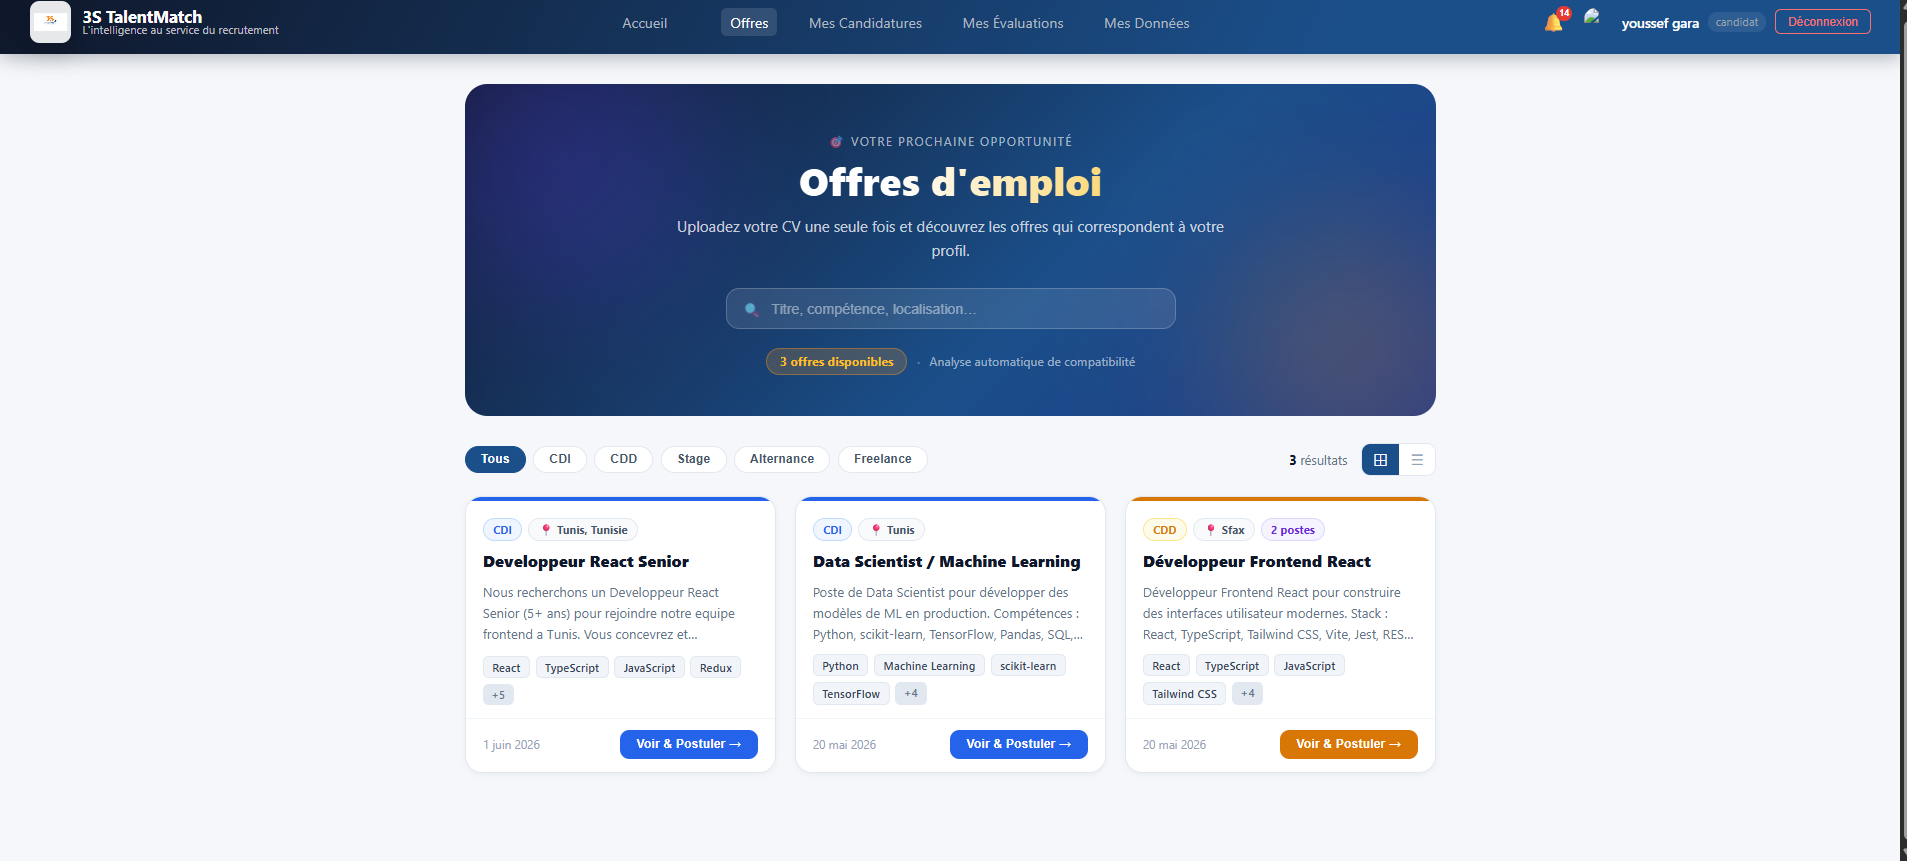
\includegraphics[width=0.9\textwidth]{captures/candidat.png}
  \caption{Consultation des offres d'emploi côté candidat}
  \label{fig:offres-candidat}
\end{figure}

La figure~\ref{fig:creation-offre} montre le formulaire de création d'une offre côté administrateur : saisie du titre, du descriptif, des compétences requises (avec leur poids respectif), des années d'expérience minimales, du niveau de formation et du domaine métier. Ces champs structurés sont directement exploités par le moteur de matching lors du calcul des scores.

\begin{figure}[H]
  \centering
  
\includegraphics[width=0.9\textwidth]{captures/creation_offre.png}
  \caption{Formulaire de création d'une offre d'emploi (vue administrateur)}
  \label{fig:creation-offre}
\end{figure}

\subsection{Moteur de matching : rôle de chaque composant IA}

Le moteur de matching combine trois composants d'intelligence artificielle complémentaires, chacun avec un rôle précis. La figure~\ref{fig:pipeline-matching} présente une vue d'ensemble du pipeline : à partir du profil candidat et de l'offre, quatre scores par critère sont calculés (compétences, sémantique, expérience, formation), puis fusionnés --- sous pondérations adaptatives et garde-fous métier --- en un score final explicable qui alimente le classement.

\begin{figure}[H]
  \centering
  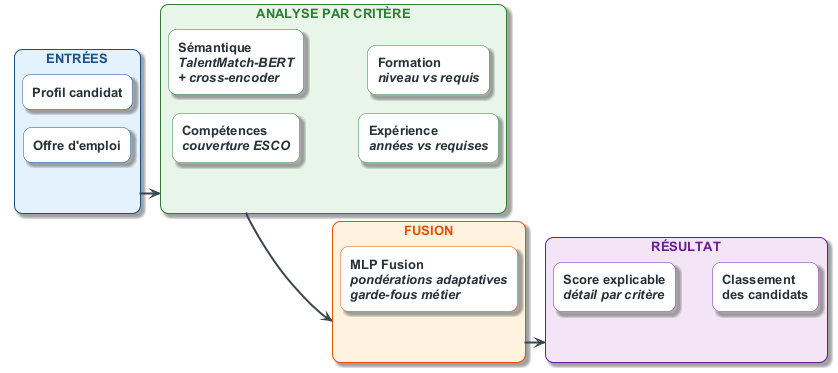
\includegraphics[width=\textwidth]{diagrams/pipeline_matching.png}
  \caption{Pipeline du moteur de matching : de l'analyse par critère à la fusion du score}
  \label{fig:pipeline-matching}
\end{figure}

\subsubsection{BGE-M3 : encodage sémantique}

\textbf{BGE-M3} est un modèle d'\textit{embeddings} multilingue : il transforme un texte (le CV, l'offre, ou une compétence isolée) en un vecteur numérique de haute dimension qui capture son \textbf{sens}, indépendamment des mots exacts employés. Deux textes proches sémantiquement produisent des vecteurs proches (mesure par similarité cosinus), ce qui permet au moteur de reconnaître qu'un « développeur front-end React » correspond à une offre « ingénieur JavaScript côté client » alors qu'aucun mot n'est identique. Ce composant a été \textbf{affiné} (\textit{fine-tuning}) sur des triplets métier (offre, bon CV, mauvais CV) construits à partir de notre corpus, afin de spécialiser la notion de proximité au domaine du recrutement --- le modèle résultant est nommé \textbf{TalentMatch-BERT}. Le choix de BGE-M3 répond aussi à la contrainte de confidentialité : le modèle s'exécute entièrement en local, aucun CV n'est transmis à un service externe.

\paragraph{Construction du jeu d'affinage.} L'affinage a nécessité la construction d'un jeu de données métier : 1\,870 triplets (offre, CV pertinent, CV non pertinent) générés à partir du corpus de CV réels et d'offres représentatives des domaines de l'entreprise. Pour chaque offre, les CV pertinents sont des profils du même métier au bon niveau, et les CV non pertinents sont choisis pour être \textit{difficiles} : profils de domaines voisins ou partageant des mots-clés avec l'offre, afin que le modèle apprenne des distinctions fines plutôt que des séparations évidentes. L'entraînement optimise une fonction de perte contrastive qui rapproche l'offre du bon CV et l'éloigne du mauvais dans l'espace vectoriel.

\subsubsection{Cross-encoder : re-classement fin}

Là où BGE-M3 encode chaque texte \textit{séparément}, le \textbf{cross-encoder} (BGE-reranker-v2-m3) lit \textbf{conjointement} la paire (offre, CV) : les deux textes traversent ensemble le même réseau, ce qui lui permet de modéliser les interactions fines entre les exigences de l'offre et le contenu du CV. Plus précis mais plus coûteux, il n'est pas utilisé pour balayer toute la base : il intervient en \textbf{re-classement} pour affiner la composante sémantique du score des candidats. Ce schéma bi-encodeur puis cross-encodeur est l'architecture de référence en recherche d'information moderne.

\subsubsection{Réseau de neurones MLP Fusion : fusion des scores}

Le score final ne repose pas que sur la sémantique : le moteur calcule également un taux de couverture des \textbf{compétences} requises (avec équivalences par domaine : détecter « EC2 » vaut « AWS »), un score d'\textbf{expérience} (années du candidat vs années requises) et un score de \textbf{formation} (niveau d'études vs niveau requis). Un \textbf{réseau de neurones MLP} (perceptron multicouche) apprend à \textbf{fusionner} ces signaux en un score unique [0,1], en capturant des interactions qu'une simple moyenne pondérée ignorerait. En complément, une formule calibrée de secours (40\,\% compétences, 25\,\% sémantique, 20\,\% expérience, 15\,\% formation) garantit un fonctionnement dégradé si les poids du MLP sont indisponibles, et des \textbf{pondérations adaptatives} ajustent l'importance relative des critères selon la séniorité de l'offre (pour un stage, la formation pèse davantage ; pour un poste senior, l'expérience domine). Enfin, des garde-fous métier plafonnent le score en cas d'incompatibilité forte (par exemple un écart de formation rédhibitoire ou un domaine ISCO-08 sans rapport), afin d'éviter les faux positifs purement sémantiques.

\subsection{Détection de domaine et garde-fous métier}

Un risque connu des systèmes de matching purement sémantiques est le \textbf{faux positif inter-domaines} : un CV rédigé avec un vocabulaire proche de l'offre peut obtenir un bon score alors que le métier n'a aucun rapport. Pour s'en prémunir, le moteur détecte le \textbf{domaine métier} du candidat et de l'offre en s'appuyant sur la classification internationale \textbf{ISCO-08} via le référentiel ESCO : le titre du poste, les expériences récentes et les compétences sont projetés sur cette classification, et une ontologie de repli couvre les intitulés non reconnus. Lorsque les domaines détectés sont incompatibles, ou lorsque l'écart entre le niveau de formation requis et celui du candidat est rédhibitoire, un \textbf{plafond} est appliqué au score final : le profil reste visible mais ne peut plus être surclassé. Ces garde-fous, ajoutés à la suite des premiers tests de la revue de sprint, ont éliminé les faux positifs observés.

\subsection{Calcul et explication du score}

Chaque exécution du matching produit, en plus du score global, une \textbf{décomposition par critère} persistée avec le match : compétences couvertes et manquantes, score d'expérience, score de formation, similarité sémantique, pondérations appliquées et alertes éventuelles (incompatibilité de domaine, formation insuffisante, expériences non détectées). Un \textbf{niveau de confiance} accompagne chaque score : il signale au recruteur les cas où le profil extrait est incomplet et où le score doit être interprété avec prudence. Cette transparence répond à un besoin opérationnel (le recruteur doit pouvoir justifier une présélection) et à une exigence de responsabilité : la décision finale reste humaine, le système fournit une aide argumentée et vérifiable, non un verdict.

La figure~\ref{fig:matching} illustre cette restitution : pour chaque candidat, le score global est accompagné du détail par critère (compétences, expérience, formation, sémantique), des compétences obligatoires couvertes ou manquantes, d'alertes éventuelles et d'un niveau de confiance.

\begin{figure}[H]
  \centering
  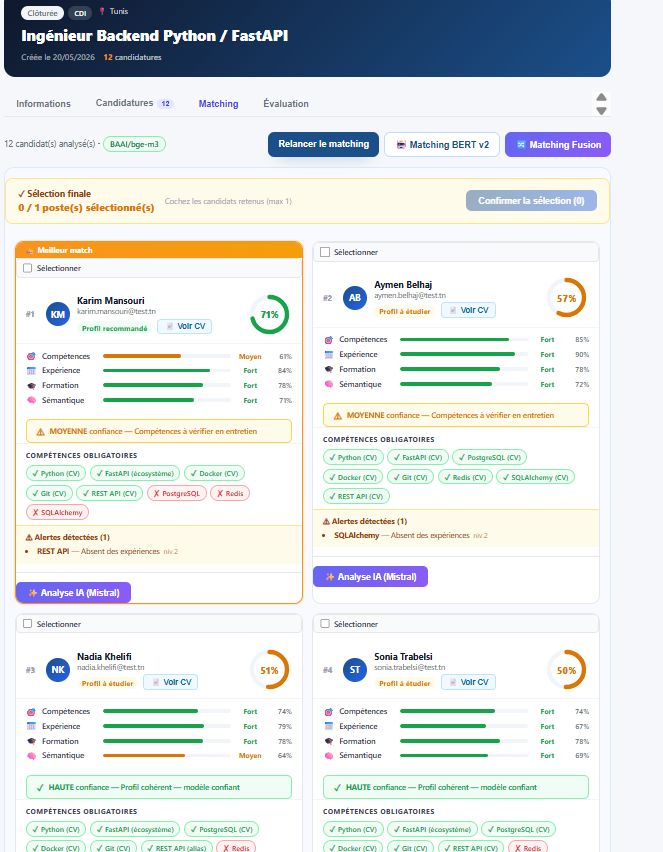
\includegraphics[width=0.9\textwidth]{captures/resultats_matching.png}
  \caption{Classement des candidats pour une offre avec explication du score}
  \label{fig:matching}
\end{figure}

\subsection{Classement des candidats et dashboard RH}

Pour chaque offre, les candidats sont classés par score décroissant, avec accès direct au profil extrait et au détail du score. Le recruteur peut alors constituer sa \textbf{sélection finale} : les candidats retenus deviennent éligibles au lancement d'une évaluation technique (chapitre~5), ce qui inscrit le matching dans un processus de décision complet plutôt qu'en outil isolé.

Le \textbf{dashboard RH} (US11) complète cette vue opérationnelle par une vision globale de l'activité de recrutement, organisée en plusieurs blocs :

\begin{itemize}
  \item \textbf{Indicateurs clés} : nombre de candidats, offres totales et actives, matchings exécutés, score moyen, nombre d'utilisateurs ;
  \item \textbf{Qualité des scores} : répartition des matchings en trois zones (excellent $\geq$\,65\,\%, moyen 35--65\,\%, faible $<$\,35\,\%), qui renseigne sur l'adéquation globale du vivier de candidats aux offres publiées ;
  \item \textbf{Pipeline par offre} : pour chaque offre, le nombre de candidats, le meilleur score et le score moyen --- le recruteur repère d'un coup d'\oe il les offres bien pourvues et celles en difficulté ;
  \item \textbf{Statuts et décisions} : répartition des candidatures (en attente, acceptées, refusées) et taux d'acceptation ;
  \item \textbf{Meilleurs profils et activité récente} : les candidats les mieux classés toutes offres confondues, et l'activité des sept derniers jours (CV déposés, matchings lancés).
\end{itemize}

La figure~\ref{fig:dashboard} présente ce tableau de bord : indicateurs globaux, qualité des scores de matching, pipeline par offre, meilleurs profils et activité récente.

\begin{figure}[H]
  \centering
  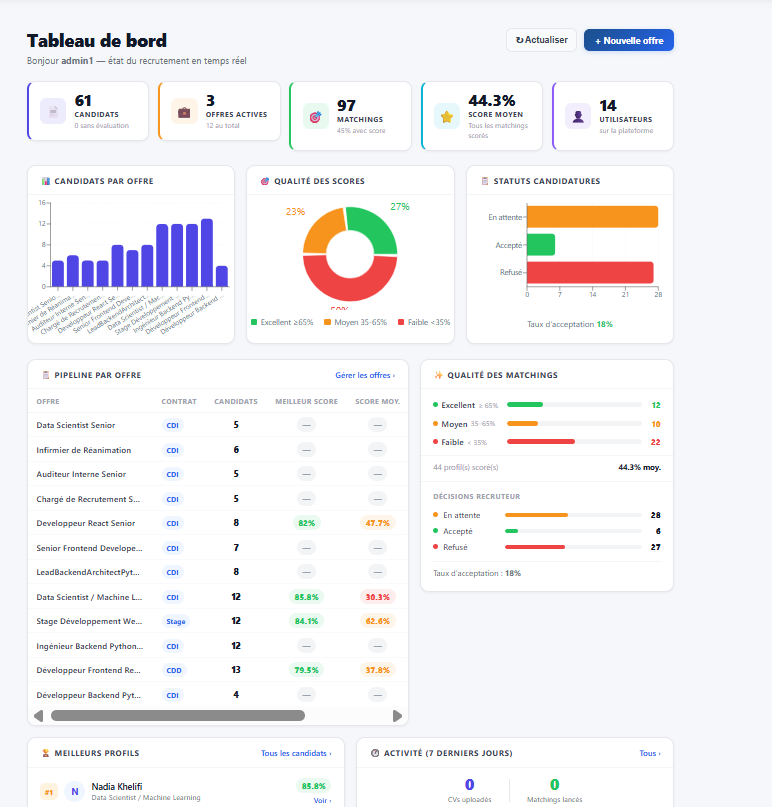
\includegraphics[width=0.85\textwidth]{captures/dashboard.png}
  \caption{Dashboard RH : indicateurs globaux de l'activité de recrutement}
  \label{fig:dashboard}
\end{figure}

\subsection{Panneau d'administration}

L'administrateur dispose d'un espace dédié pour piloter la plateforme. Ses principales fonctions sont la gestion des comptes utilisateurs (création, activation, désactivation, modification des rôles), la supervision des offres d'emploi de l'ensemble de l'organisation et l'assignation des recruteurs aux offres. Cette gouvernance centralisée garantit que chaque recruteur accède uniquement aux offres qui lui ont été explicitement confiées, et que les données des candidats ne circulent pas en dehors du périmètre autorisé.

La figure~\ref{fig:admin-users} présente le panneau de gestion des utilisateurs : liste des comptes avec rôle, statut d'activation, date de création, et actions possibles (édition, désactivation, suppression).

\begin{figure}[H]
  \centering
  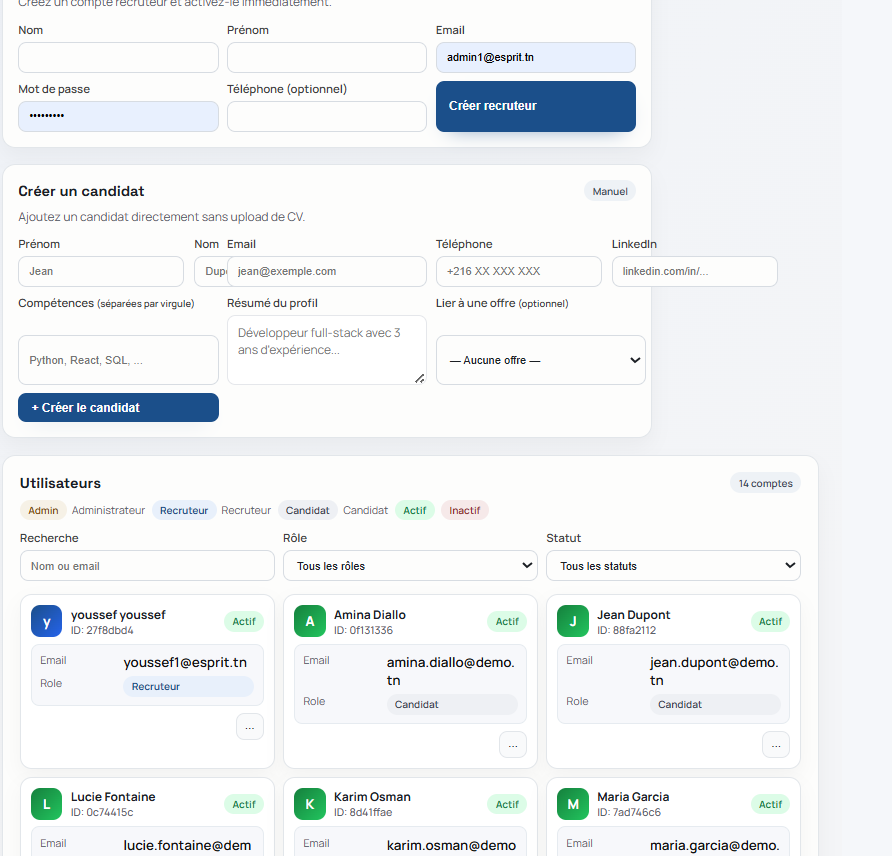
\includegraphics[width=0.9\textwidth]{captures/admin_users.png}
  \caption{Panneau d'administration : gestion des utilisateurs et des rôles}
  \label{fig:admin-users}
\end{figure}

\section{Tests et validation du sprint}

La validation du moteur de matching a reposé sur une \textbf{validation croisée à 5 plis} (\textit{k-fold}) sur un jeu de \textbf{1\,870 triplets} (offre, CV pertinent, CV non pertinent) construits à partir du corpus de CV réels multi-domaines. Trois indicateurs standard de la recherche d'information ont été mesurés : l'\textbf{accuracy de triplet} (le CV pertinent obtient-il un meilleur score que le CV non pertinent ?), le \textbf{MRR} (\textit{Mean Reciprocal Rank} : le bon CV est-il classé en tête ?) et la \textbf{marge} (écart moyen de score entre bon et mauvais CV, qui mesure la confiance de la séparation). Le tableau~\ref{tab:metriques-s3} compare le modèle BGE-M3 de base au modèle affiné TalentMatch-BERT.

\begin{table}[H]
\centering
\caption{Validation croisée (5 plis, 1\,870 triplets) du moteur de matching}
\label{tab:metriques-s3}
\small
\begin{tabularx}{\textwidth}{X r r r}
\rowcolor{tabheader}
\textcolor{white}{\textbf{Modèle}} & \textcolor{white}{\textbf{Accuracy}} & \textcolor{white}{\textbf{MRR}} & \textcolor{white}{\textbf{Marge}} \\
BGE-M3 de base (sans affinage) & 77,9\,\% $\pm$ 1,6 & 0,937 & 0,149 \\
\rowcolor{tabalt}
\textbf{TalentMatch-BERT (affiné)} & \textbf{100\,\%} $\pm$ 0,0 & \textbf{1,000} & \textbf{0,670} \\
\bottomrule
\end{tabularx}
\end{table}

L'affinage sur triplets métier apporte un gain décisif : le modèle affiné sépare correctement \textbf{100\,\%} des 1\,870 triplets sur les cinq plis (écart-type nul, comportement stable), et la marge de séparation est multipliée par 4,5 --- le modèle ne se contente pas de bien classer, il classe avec confiance. En complément, des scénarios de bout en bout (offres réelles avec candidats de pertinence connue) ont confirmé que le classement produit correspond au classement attendu par un évaluateur humain, avec une \textbf{corrélation de Spearman comprise entre 0,90 et 1,00} selon les scénarios.

\smallskip
\noindent\textit{Note méthodologique} : pour une tâche de \textbf{classement} (ranking), les indicateurs standards sont l'accuracy de triplet, le MRR et la corrélation de Spearman --- et non la précision/rappel/F1, lesquels s'appliquent à une classification binaire à seuil fixe. Ces trois indicateurs sont ceux utilisés dans la littérature de recherche d'information (TREC, BEIR) pour évaluer les modèles d'embeddings.

\section{Revue du sprint}

La démonstration du matching sur des offres réelles a validé le c\oe ur du sprint. Deux retours principaux ont orienté la suite : d'une part, la nécessité de \textbf{plafonner les scores} en cas d'incompatibilité de domaine ou de formation (un profil sémantiquement proche mais hors métier pouvait être surclassé), garde-fous intégrés au moteur au cours du sprint ; d'autre part, le constat qu'un bon score de matching ne garantit pas que les compétences \textbf{déclarées} dans le CV soient réellement \textbf{maîtrisées} --- constat qui a directement motivé le module d'évaluation technique du Sprint~4.

\section{Conclusion du sprint}

Le Sprint~3 a livré le c\oe ur intelligent de la plateforme : un moteur de matching local, multi-critères et explicable, validé par une évaluation rigoureuse (100\,\% d'accuracy en validation croisée sur 1\,870 triplets), ainsi que le classement des candidats et le dashboard RH. La plateforme sait désormais dire \textit{qui correspond le mieux à une offre et pourquoi} ; le sprint suivant s'attache à vérifier \textit{ce que les candidats savent réellement faire}, via le module d'évaluation technique.
\newpage

\chapter{Sprint 4 : Module d'évaluation, sécurité et finalisation}

\section{Introduction}

Ce chapitre décrit la réalisation du Sprint~4 (semaines 15 à 18), qui achève la plateforme sur trois axes. Le premier est le \textbf{module d'évaluation technique} : né du constat de la revue du Sprint~3, il vérifie que les compétences déclarées dans un CV sont réellement maîtrisées, en faisant passer au candidat un test en ligne noté par les composants d'IA locaux de la plateforme. Le deuxième axe est la \textbf{sécurité et la protection des données personnelles}, transverse à l'ensemble du système. Le troisième est la \textbf{finalisation} : notifications, invitations, tests d'intégration et validation globale.

\section{Planification du sprint}

\subsection{Objectif du sprint}

L'objectif du Sprint~4 est double : livrer un module d'évaluation complet --- du lancement par le recruteur jusqu'au rapport d'analyse final, en passant par la passation sécurisée du test par le candidat --- et consolider la plateforme sur le plan de la sécurité, de la protection des données personnelles et de la traçabilité, l'ensemble devant fonctionner \textbf{entièrement en local}, sans aucun appel à un service d'IA externe.

\subsection{Backlog du sprint}

Le tableau~\ref{tab:backlog-s4} présente les user stories du sprint, et le tableau~\ref{tab:taches-s4} leur découpage en tâches techniques.

\begin{table}[H]
\centering
\caption{User stories du Sprint 4}
\label{tab:backlog-s4}
\small
\begin{tabularx}{\textwidth}{>{\bfseries}p{0.9cm} p{1.9cm} X X p{1.4cm}}
\rowcolor{tabheader}
\textcolor{white}{\textbf{ID}} & \textcolor{white}{\textbf{En tant que\ldots}} & \textcolor{white}{\textbf{Je veux\ldots}} & \textcolor{white}{\textbf{Afin de\ldots}} & \textcolor{white}{\textbf{Priorité}} \\
US12 & RH & lancer les évaluations techniques (invitation e-mail, code PIN, dates) & vérifier les compétences des candidats retenus & Haute \\
\rowcolor{tabalt}
US13 & Candidat & passer mon évaluation en ligne (QCM adaptatif, questions rédigées) & démontrer mes compétences réelles & Haute \\
US14 & RH & consulter le rapport d'évaluation IA et la cohérence CV--test & prendre une décision éclairée & Haute \\
\rowcolor{tabalt}
US15 & RH & disposer d'un score d'intégrité durant l'évaluation & détecter les comportements suspects & Moyenne \\
US16 & Candidat & recevoir des notifications (e-mail et plateforme) & suivre l'avancement de ma candidature & Moyenne \\
\rowcolor{tabalt}
US17 & Admin & consulter les journaux d'accès aux données & tracer l'accès aux données personnelles & Moyenne \\
\bottomrule
\end{tabularx}
\end{table}

\begin{table}[H]
\centering
\caption{Découpage en tâches techniques du Sprint 4}
\label{tab:taches-s4}
\small
\begin{tabularx}{\textwidth}{>{\bfseries}p{1.2cm} X}
\rowcolor{tabheader}
\textcolor{white}{\textbf{US}} & \textcolor{white}{\textbf{Tâches techniques}} \\
US12 & Génération locale des questionnaires par offre (LLM Ollama, arrière-plan, cache) ; panneau de lancement multi-candidats (dates, questions du recruteur) ; invitation différée envoyée uniquement quand le questionnaire est prêt. \\
\rowcolor{tabalt}
US13 & Page de passation candidat (accès par compte + code PIN, fenêtre temporelle) ; QCM adaptatif (IRT) ; questions rédigées ; mode examen (plein écran, minuterie par question). \\
US14 & Notation sémantique locale (BGE-M3) ; calcul de l'écart déclaré--démontré ; rapport d'analyse généré par LLM local ; radar Déclaré vs Démontré ; onglet Évaluations (liste, détail, réponses). \\
\rowcolor{tabalt}
US15 & Télémétrie de passation (sorties de plein écran, changements d'onglet, collages, temps de réponse, frappes) ; calcul du score d'intégrité 0--100. \\
US16 & Notifications internes + e-mails transactionnels (invitation avec PIN, changements de statut). \\
\rowcolor{tabalt}
US17 & Journal des accès (\texttt{access\_logs}) : qui a consulté quelle ressource, quand, depuis quelle adresse. \\
\bottomrule
\end{tabularx}
\end{table}

\section{Réalisation du sprint}

\subsection{Module d'évaluation technique des candidats}

Le module d'évaluation suit un parcours en quatre temps : le recruteur \textbf{lance} l'évaluation depuis les résultats du matching (sélection d'un ou plusieurs candidats, définition de la fenêtre de passage et d'éventuelles questions personnelles) ; le candidat \textbf{reçoit} une invitation par e-mail avec un code PIN à usage unique ; il \textbf{passe} le test en ligne depuis son espace personnel ; le recruteur \textbf{consulte} les résultats analysés. Quatre briques techniques soutiennent ce parcours.

\begin{figure}[H]
  \centering
  
\includegraphics[width=0.75\textwidth]{captures/lancement_evaluation.png}
  \caption{Panneau de lancement des évaluations côté recruteur (fenêtre de passage et questions personnalisées)}
  \label{fig:lancement-eval}
\end{figure}

\subsubsection{Génération locale des questionnaires (Ollama)}

Plutôt qu'une banque de questions figée --- inadaptée à la variété des offres ---, les questionnaires sont \textbf{générés dynamiquement} pour chaque offre par un modèle de langage exécuté \textbf{en local} via Ollama. Seuls les noms de compétences sont transmis au modèle : aucun contenu de CV ne sort de la plateforme. La génération applique des règles de qualité strictes : répartition des QCM par paliers de difficulté (moitié faciles à moyens, moitié difficiles), distracteurs plausibles obligatoires, et \textbf{auto-vérification} --- le modèle répond à chaque question générée sans voir la réponse attendue, et tout désaccord entraîne le rejet de la question. Les questions ouvertes sont des mises en situation de \textbf{raisonnement} (résolution de problème, analyse), non de simples définitions. La génération étant coûteuse (environ une minute par compétence), elle s'exécute \textbf{en arrière-plan} dès le lancement, avec mise en \textbf{cache} par offre : le premier lancement prépare un pool de questions, les suivants sont instantanés, et chaque candidat reçoit un sous-ensemble différent tiré de ce pool.

\subsubsection{QCM adaptatif (théorie de réponse à l'item)}

La partie QCM applique la \textbf{théorie de réponse à l'item} (IRT), le cadre statistique des tests standardisés adaptatifs : chaque question porte des paramètres de difficulté et de discrimination, et le niveau du candidat est modélisé par une variable latente $\theta$ ré-estimée après chaque réponse. Le test est \textbf{adaptatif} : la question suivante est choisie au plus près du niveau estimé courant, ce qui permet de converger vers une mesure fiable en une dizaine de questions --- un candidat fort reçoit rapidement des questions difficiles, un candidat faible n'est pas noyé. Le niveau final est projeté sur une échelle 0--10 par compétence.

\subsubsection{Notation sémantique des réponses rédigées}

Les réponses aux questions ouvertes sont notées par \textbf{similarité sémantique} : pour chaque question, trois réponses de référence de qualité croissante (faible, correcte, experte) sont générées et encodées avec \textbf{BGE-M3} --- le même modèle que le matching, réutilisé ici. La réponse du candidat est encodée à son tour et positionnée par rapport aux trois références (similarité cosinus), produisant un score 0--100. Une pénalité s'applique aux réponses trop courtes pour être évaluables. Le score n'est pas révélé au candidat pendant le test, afin de ne pas influencer ses réponses suivantes.

La figure~\ref{fig:test-candidat} montre la passation côté candidat : plein écran, minuterie visible, difficulté de la question affichée et copier-coller désactivé.

\begin{figure}[H]
  \centering
  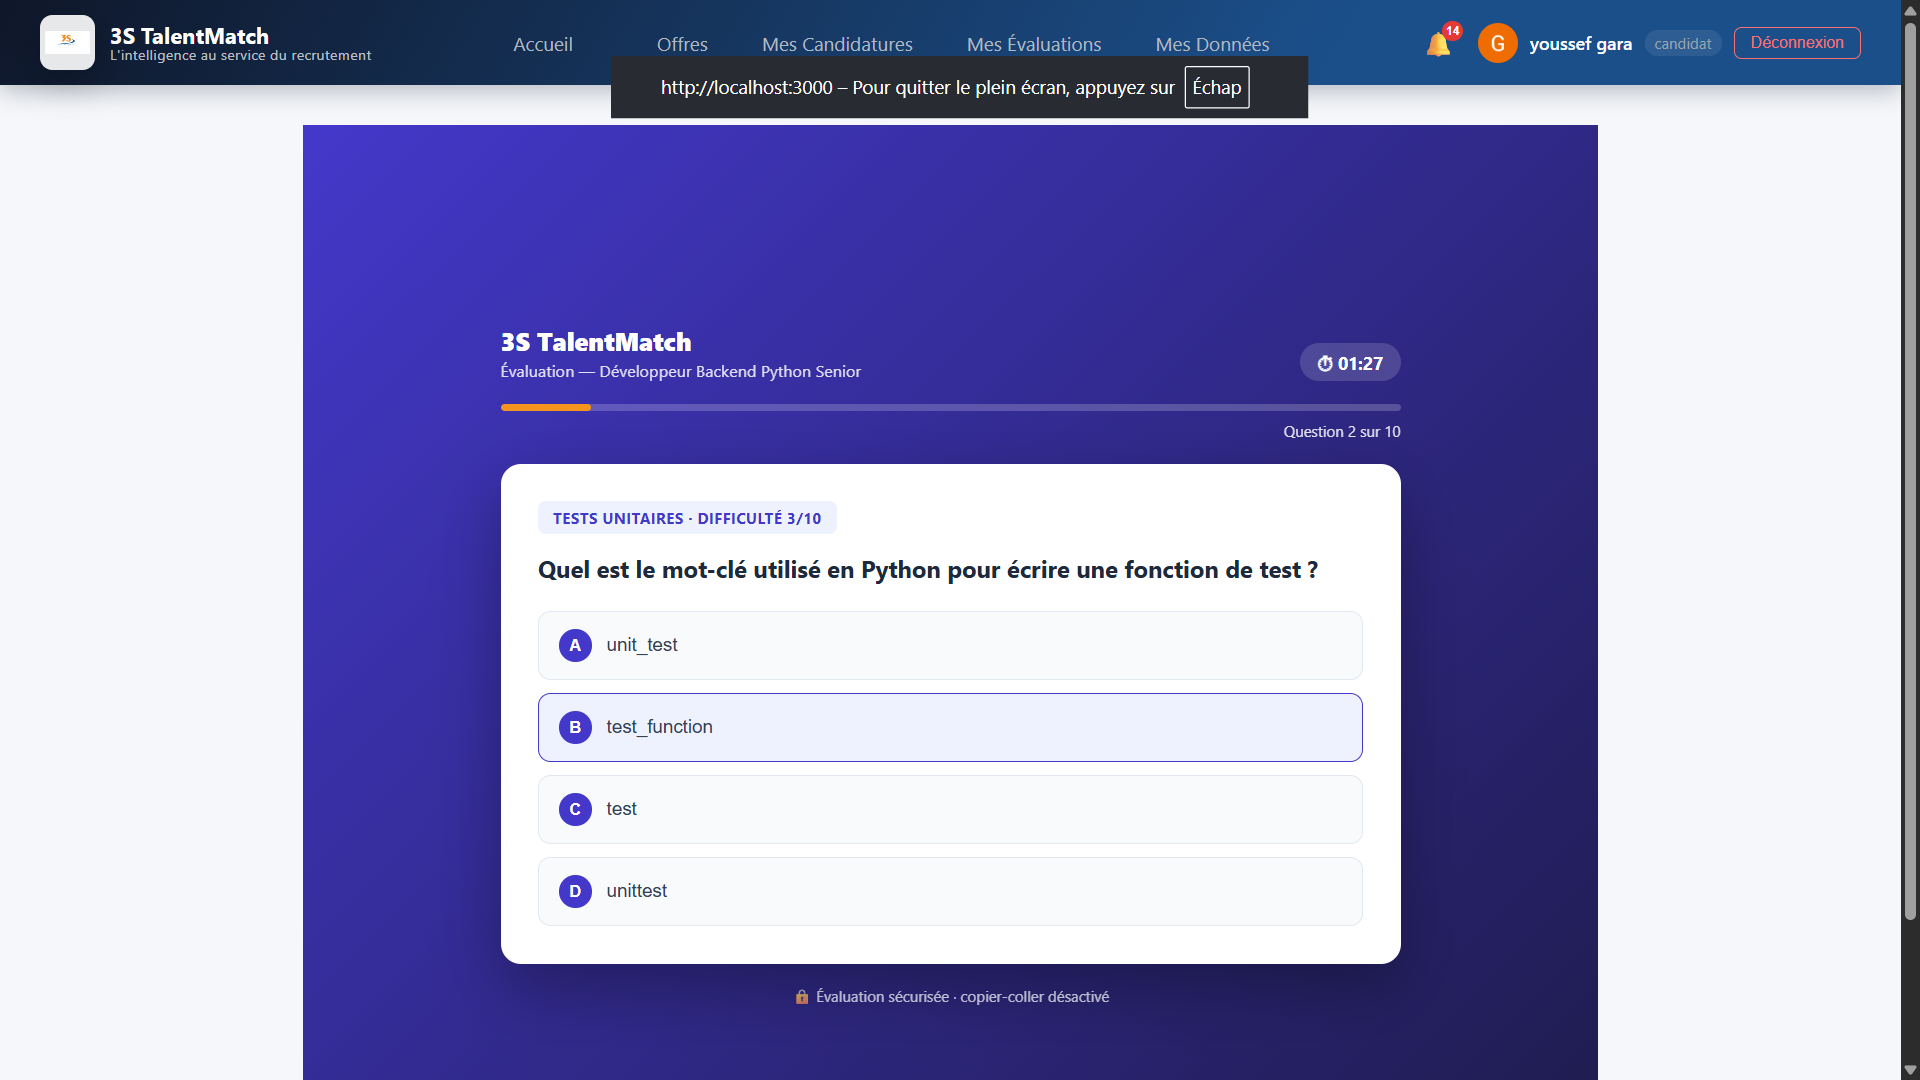
\includegraphics[width=0.9\textwidth]{captures/test_candidat.png}
  \caption{Passation du test côté candidat (mode examen, QCM avec minuterie)}
  \label{fig:test-candidat}
\end{figure}

\subsubsection{Écart déclaré--démontré et rapport d'évaluation IA}

L'apport central du module est la confrontation entre ce que le CV \textbf{déclare} et ce que le test \textbf{démontre}. Le niveau déclaré de chaque compétence est dérivé du CV parsé (présence de la compétence, usage effectif dans les expériences, séniorité du profil) ; le niveau démontré provient du test. L'écart moyen pondéré par l'importance de chaque compétence dans l'offre produit un indicateur de \textbf{cohérence CV--test} (0--100), classé en trois zones : cohérent, à vérifier, écart important. Cet indicateur vient moduler le score de matching : un profil bien classé mais dont le test contredit le CV est signalé au recruteur. Enfin, un \textbf{rapport d'analyse} est généré par le LLM local à partir de l'ensemble des résultats (niveau technique, qualité du raisonnement dans les réponses rédigées, cohérence CV--test) et se conclut par une recommandation argumentée --- recruter, approfondir ou écarter --- présentée avec un \textbf{radar Déclaré vs Démontré} par compétence. La décision finale appartient toujours au recruteur, qui dispose de l'intégralité des réponses du candidat pour se forger sa propre opinion.

La figure~\ref{fig:radar-eval} présente les résultats de l'évaluation tels qu'ils sont restitués au recruteur : un radar par compétence superposant le niveau déclaré (CV) et le niveau démontré (test), l'indicateur de cohérence CV--test, et un extrait du rapport d'analyse généré par le LLM local.

\begin{figure}[H]
  \centering
  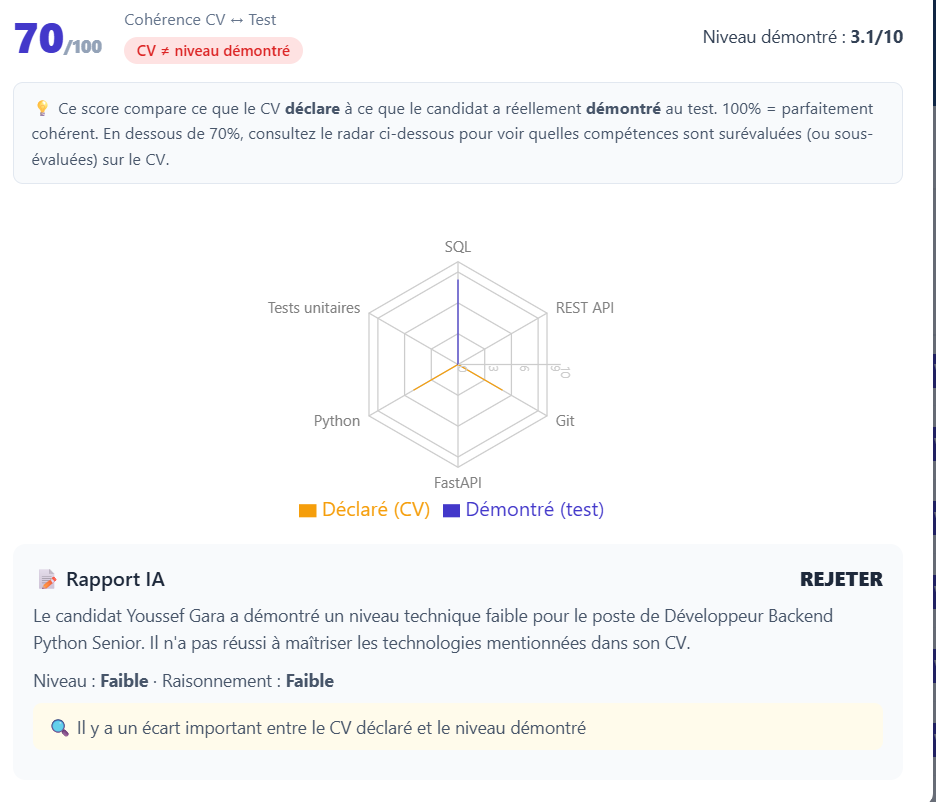
\includegraphics[width=0.85\textwidth]{captures/radar_evaluation.png}
  \caption{Résultats d'évaluation : radar Déclaré vs Démontré et rapport d'analyse IA}
  \label{fig:radar-eval}
\end{figure}

\subsection{Sécurité et gestion des rôles}

La sécurité de la plateforme s'organise en trois niveaux : la sécurité applicative générale, le contrôle d'accès par rôle, et le mode examen spécifique aux évaluations.

\subsubsection{Sécurité applicative}

Au niveau de l'API, toutes les entrées sont \textbf{validées par des schémas Pydantic} avant tout traitement : types, formats et champs obligatoires sont vérifiés automatiquement, ce qui neutralise une large classe d'attaques par données malformées. L'accès à la base de données passe exclusivement par l'ORM SQLAlchemy avec requêtes paramétrées, ce qui écarte les injections SQL. Les fichiers téléversés sont contrôlés (type et taille) avant traitement. Les jetons JWT sont signés avec une clé secrète serveur et une durée de validité limitée ; toute requête portant un jeton absent, invalide ou expiré est rejetée avec le code \texttt{401}, et le frontend déconnecte alors automatiquement l'utilisateur --- ce comportement est centralisé dans l'unique client HTTP de l'application, ce qui en fait un invariant.

\subsubsection{Contrôle d'accès par rôle et par propriété}

Chaque endpoint applique une double vérification, conformément à la matrice des permissions (tableau~\ref{tab:matrice-roles}) : le \textbf{rôle} (un candidat ne peut pas appeler un endpoint recruteur --- rejet \texttt{403}) et la \textbf{propriété de la ressource} (un recruteur n'accède qu'aux offres qui lui sont assignées et à leurs évaluations ; un candidat n'accède qu'à ses propres sessions, vérifiées par le lien entre son compte et son profil candidat). Ce second contrôle est essentiel : le rôle seul ne suffit pas, car deux recruteurs ne doivent pas voir les données l'un de l'autre.

\subsubsection{Mode examen de l'évaluation}

La passation du test est encadrée par un dispositif complet :

\begin{itemize}
  \item \textbf{Double facteur d'accès} : connexion au compte candidat propriétaire \textbf{et} code PIN à usage unique reçu par e-mail --- le lien seul ne suffit pas, même intercepté ;
  \item \textbf{Fenêtre temporelle} : accès refusé avant la date d'ouverture et après l'échéance définies par le recruteur (rejet \texttt{403} sur toute tentative de réponse hors fenêtre) ;
  \item \textbf{Règles explicites} : un écran présente les règles de passation, que le candidat accepte par un clic explicite avant que le plein écran ne s'active --- aucune règle n'est appliquée sans avoir été annoncée ;
  \item \textbf{Conditions d'examen} : plein écran, minuterie par question QCM (une réponse non donnée à temps est comptée comme absente), copier-coller désactivé.
\end{itemize}

En parallèle, une \textbf{télémétrie de passation} enregistre les signaux listés dans le tableau~\ref{tab:signaux-integrite}, agrégés en un \textbf{score d'intégrité} 0--100 présenté au recruteur (US15).

\begin{table}[H]
\centering
\caption{Signaux de télémétrie agrégés dans le score d'intégrité}
\label{tab:signaux-integrite}
\small
\begin{tabularx}{\textwidth}{p{4.5cm} X}
\rowcolor{tabheader}
\textcolor{white}{\textbf{Signal collecté}} & \textcolor{white}{\textbf{Ce qu'il peut indiquer}} \\
Sorties du mode plein écran & Consultation d'une autre application ou d'un autre écran \\
\rowcolor{tabalt}
Changements d'onglet / perte de focus & Recherche de la réponse dans un autre onglet \\
Tentatives de collage & Insertion d'un texte préparé ou copié ailleurs \\
\rowcolor{tabalt}
Temps de réponse très court sur une question difficile & Réponse connue à l'avance ou obtenue par un tiers \\
Incohérence frappes clavier / longueur du texte final & Texte injecté sans avoir été tapé (dictée d'un assistant IA, collage contourné) \\
\rowcolor{tabalt}
Rythme d'écriture anormalement régulier & Recopie d'un texte existant plutôt que rédaction spontanée \\
\bottomrule
\end{tabularx}
\end{table}

Un choix de conception important a été retenu : \textbf{aucune sanction automatique}. Chaque signal pris isolément est ambigu --- une touche Échap ou un rafraîchissement de page ne prouvent rien --- et les premiers essais réels ont confirmé le risque de faux positifs. La plateforme trace et informe, mais c'est le \textbf{recruteur} qui juge, sur la base du score d'intégrité et du détail des incidents : c'est le modèle de fonctionnement des solutions professionnelles de surveillance d'examen à distance.

\subsection{Mesures de protection des données personnelles}

\subsubsection{Contexte et enjeux}

Un CV est, par nature, un concentré de données personnelles : identité, coordonnées, parcours professionnel et académique, parfois photographie. Une plateforme de recrutement traite en outre des données produites par elle-même --- scores de matching, résultats d'évaluation, signaux d'intégrité --- qui concernent directement les personnes. Le traitement de ces données s'inscrit dans un cadre juridique exigeant : en Tunisie, la loi organique n°2004-63 relative à la protection des données à caractère personnel, sous le contrôle de l'INPDP (Instance Nationale de Protection des Données Personnelles) ; et, pour toute interaction avec des candidats européens, les principes portés par le règlement général européen sur la protection des données. Sans prétendre à un audit juridique de conformité, le projet a intégré dès sa conception des \textbf{mesures concrètes de protection}, organisées ci-dessous selon les grands principes de protection des données.

\subsubsection{Minimisation et traitement local}

Le principe de minimisation veut que chaque composant n'accède qu'aux données strictement nécessaires à sa fonction. Deux mesures structurantes l'appliquent :

\begin{itemize}
  \item \textbf{Traitement 100\,\% local} : extraction, parsing, matching, génération de questionnaires, notation et rapports s'exécutent intégralement sur l'infrastructure de l'entreprise. Aucune donnée de candidat n'est transmise à un service d'IA externe --- c'est la raison du choix d'Ollama, de BGE-M3 et de spaCy en local, et de l'abandon de toute API d'IA distante ;
  \item \textbf{Minimisation vis-à-vis du LLM} : même en local, le générateur de questionnaires ne reçoit que des \textit{noms de compétences}, jamais le contenu d'un CV ni l'identité d'un candidat.
\end{itemize}

\subsubsection{Information et transparence}

Au moment du dépôt de son CV, le candidat est informé par une mention explicite de l'utilisation qui sera faite de ses données (analyse automatisée du CV dans le cadre du processus de recrutement, accès limité aux équipes concernées). Sa prise de connaissance est enregistrée et \textbf{horodatée en base} (champs dédiés du profil candidat). Côté résultats, la transparence est aussi fonctionnelle : les scores sont expliqués, et le candidat suit l'état de sa candidature depuis son espace.

\subsubsection{Sécurité et confidentialité des accès}

Les mesures de sécurité décrites en section précédente servent directement la protection des données : authentification individuelle, moindre privilège par rôle \textbf{et} par assignation (un recruteur ne voit que les candidats de ses offres), double facteur pour l'accès aux évaluations, mots de passe hachés, jetons à durée limitée.

\subsubsection{Traçabilité des accès}

Chaque consultation de données de candidat est tracée (US17) dans la table \texttt{access\_logs} : utilisateur, rôle, action effectuée, ressource concernée, date et adresse IP. Ce journal, consultable par l'administrateur, permet de répondre à la question « qui a accédé aux données de ce candidat, quand et pour quoi faire ? » --- capacité essentielle en cas d'incident ou de demande d'une personne concernée, et dissuasive contre les consultations sans motif légitime.

\subsubsection{Droits des personnes et cycle de vie des données}

\begin{itemize}
  \item \textbf{Accès et rectification} : le candidat consulte son profil extrait et peut corriger les données mal détectées (US07) ;
  \item \textbf{Anonymisation} : un mécanisme d'anonymisation permet de masquer les informations identifiantes d'un profil tout en conservant les données statistiques utiles ;
  \item \textbf{Suppression} : les profils candidats et les sessions d'évaluation peuvent être supprimés par les ayants droit ; les suppressions en cascade sont gérées au niveau du schéma de base (contraintes \texttt{ON DELETE}), garantissant qu'aucune donnée orpheline ne subsiste ;
  \item \textbf{Limitation de la finalité} : les données collectées ne servent qu'au processus de recrutement ; les scores d'évaluation ne sont pas révélés pendant la passation et ne sont accessibles qu'aux recruteurs habilités.
\end{itemize}

\subsection{Notifications et invitations par e-mail}

Le sprint a finalisé la couche de communication : notifications internes (cloche de la plateforme) et e-mails transactionnels. L'invitation à une évaluation illustre le soin apporté au parcours : l'e-mail --- lien personnel, code PIN, dates de la fenêtre de passage --- n'est envoyé qu'au moment où le questionnaire du candidat est \textbf{effectivement prêt}. Si la génération du pool de questions est encore en cours au lancement, l'invitation est \textbf{différée automatiquement} et part dès que la préparation se termine : le candidat ne peut jamais ouvrir un test vide ou incomplet.

La figure~\ref{fig:email-invite} présente un exemple d'e-mail d'invitation : le candidat y trouve le lien personnel, son code PIN, et la fenêtre de disponibilité du test.

\begin{figure}[H]
  \centering
  
\includegraphics[width=0.75\textwidth]{captures/email_invitation.png}
  \caption{E-mail d'invitation à une évaluation (lien personnel, PIN, dates de passage)}
  \label{fig:email-invite}
\end{figure}

Au-delà des e-mails, la plateforme maintient un système de \textbf{notifications internes} : chaque événement pertinent (résultat de matching disponible, invitation envoyée, statut d'une candidature modifié) génère une notification visible depuis la cloche de la barre de navigation. Ces notifications garantissent qu'aucun acteur ne manque une action attendue, même sans consulter constamment la plateforme.

\begin{figure}[H]
  \centering
  
\includegraphics[width=0.9\textwidth]{captures/notifications.png}
  \caption{Centre de notifications internes de la plateforme}
  \label{fig:notifs}
\end{figure}

La figure~\ref{fig:mes-evals} montre la page de suivi des évaluations côté recruteur : pour chaque candidat évalué, le niveau estimé, le score d'intégrité, l'indicateur de cohérence CV--test et la progression.

\begin{figure}[H]
  \centering
  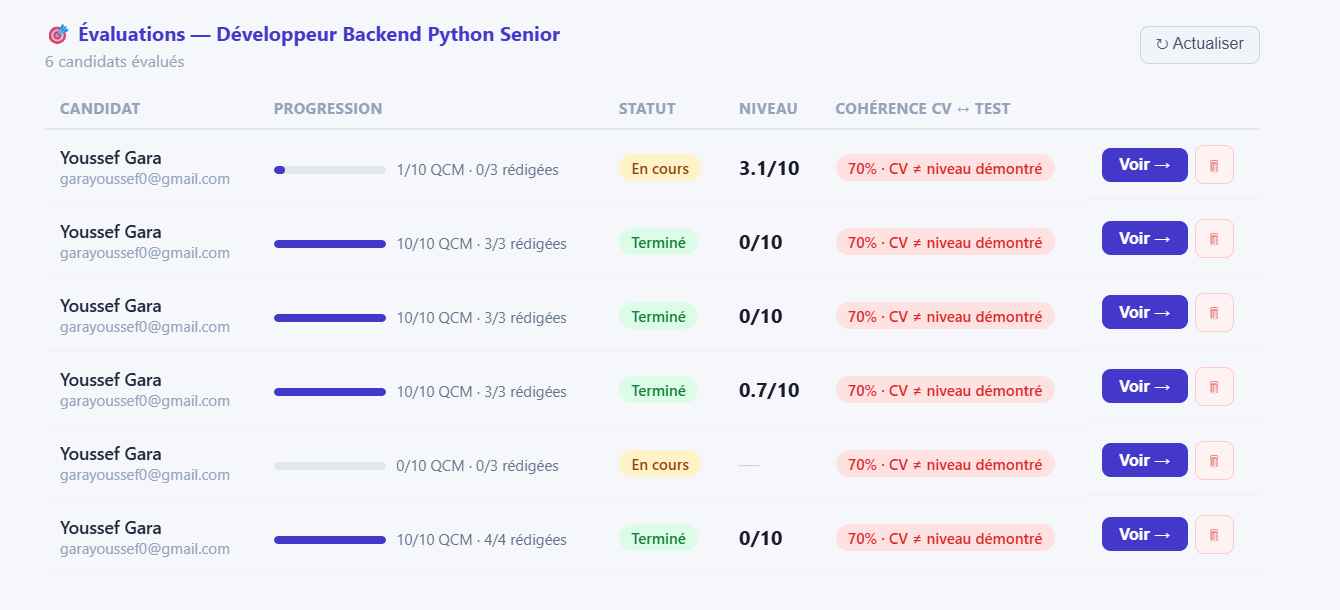
\includegraphics[width=0.9\textwidth]{captures/mes_evaluation.png}
  \caption{Suivi des évaluations : progression, niveau estimé, cohérence CV--test et intégrité}
  \label{fig:mes-evals}
\end{figure}

\section{Tests et validation du sprint}

\subsection{Tests fonctionnels et d'intégration}

Le parcours complet a été validé de bout en bout, avec des e-mails réels : lancement par le recruteur $\rightarrow$ réception de l'invitation et du PIN $\rightarrow$ connexion candidat, saisie du PIN, acceptation des règles $\rightarrow$ passation (QCM adaptatif puis questions rédigées) $\rightarrow$ calcul des scores et de la cohérence CV--test $\rightarrow$ rapport d'analyse et radar côté recruteur. Les cas limites ont été systématiquement testés : accès hors fenêtre temporelle (refusé), PIN erroné (refusé), compte non propriétaire (refusé), lancement groupé multi-candidats, suppression de session, et génération pour des compétences absentes du référentiel initial (questionnaires correctement produits, y compris hors informatique --- une offre en comptabilité a servi de contre-épreuve multi-domaines).

\subsection{Validation du moteur IA}

Chaque composant IA du module a été validé séparément, avec les résultats suivants :

\begin{table}[H]
\centering
\caption{Validation des composants IA du module d'évaluation}
\label{tab:metriques-s4}
\small
\begin{tabularx}{\textwidth}{X X}
\rowcolor{tabheader}
\textcolor{white}{\textbf{Composant testé}} & \textcolor{white}{\textbf{Résultat}} \\
Notation sémantique (BGE-M3) : trois réponses de qualité connue soumises à la même question & Réponse experte : \textbf{80}/100 ; correcte : \textbf{41}/100 ; faible : \textbf{16}/100 --- l'ordre attendu est respecté avec une séparation nette \\
\rowcolor{tabalt}
Test adaptatif (IRT) : candidat simulé de niveau connu ($\approx$\,7/10) & Niveau estimé : \textbf{6,7}/10 après une dizaine de questions --- convergence correcte \\
Auto-vérification des QCM générés & Les questions dont la réponse du vérificateur diverge sont rejetées ; répartition des difficultés conforme aux paliers demandés \\
\rowcolor{tabalt}
Performance de préparation & Génération $\approx$\,1 minute par compétence, exécutée en arrière-plan et mise en cache par offre ; lancements suivants quasi instantanés \\
\bottomrule
\end{tabularx}
\end{table}

\section{Préparation au déploiement}

La plateforme a été conçue dès le départ pour un déploiement reproductible sur tout environnement Linux. Cette section décrit les éléments mis en place pour rendre la mise en production opérationnelle.

\subsection{Conteneurisation Docker}

Chaque composant dispose d'un \texttt{Dockerfile} dédié. Le backend FastAPI est construit à partir de l'image officielle Python 3.10, installe les dépendances (\texttt{requirements.txt}), télécharge le modèle spaCy \texttt{fr\_core\_news\_md} et expose le port 8000. Le frontend React est compilé via \texttt{npm run build} dans une image Node, puis servi par Nginx. Les deux services sont orchestrés par un fichier \texttt{railway.toml} pour le déploiement sur Railway, la plateforme retenue par 3S pour l'hébergement.

\subsection{Variables d'environnement et configuration}

Toutes les valeurs sensibles (URL de la base de données, clés JWT, identifiants OAuth Google/LinkedIn, paramètres SMTP) sont externalisées dans un fichier \texttt{.env} non versionné, documenté via \texttt{.env.example}. La base de données PostgreSQL 16 est provisionnée indépendamment (service Railway ou instance dédiée) sur le port 5433.

\subsection{Migrations et initialisation}

Le schéma de base de données est géré par Alembic : la commande \texttt{alembic upgrade head} applique l'ensemble des migrations au démarrage du serveur. Un script d'amorçage (\texttt{scripts/seed\_dev\_admin.py}) crée le compte administrateur initial et les données de démonstration. Les modèles d'IA (BGE-M3, cross-encoder, spaCy) sont pré-chargés au démarrage de l'API via le gestionnaire de cycle de vie FastAPI (\texttt{lifespan}), éliminant toute latence à froid sur les premières requêtes de matching.

\subsection{Documentation technique}

L'API expose une documentation Swagger interactive à \texttt{/docs}, générée automatiquement par FastAPI à partir des schémas Pydantic. Un guide d'installation et de déploiement (Annexe B) détaille les étapes pour un développeur reprenant le projet : création du virtualenv, installation des dépendances, configuration de la base, exécution des migrations et lancement des serveurs.

\section{Revue du sprint}

La revue finale a validé le module d'évaluation comme aboutissement du projet. Deux ajustements notables sont issus des retours d'usage réels : d'une part, l'\textbf{invitation différée} (un candidat ne doit jamais recevoir un lien vers un test encore en préparation) ; d'autre part, l'abandon du blocage automatique en cas d'incident de passation au profit du \textbf{jugement humain} appuyé sur le score d'intégrité --- les premiers essais ayant montré que des gestes anodins (rafraîchissement, touche Échap) pouvaient être pris à tort pour de la triche. Ces deux décisions illustrent la ligne directrice du projet : l'IA instruit, l'humain décide.

\section{Conclusion du sprint}

Le Sprint~4 clôt le périmètre fonctionnel de la plateforme : elle sait désormais non seulement classer les candidatures (Sprint~3), mais aussi \textbf{vérifier} les compétences déclarées par un test adaptatif sécurisé, noté localement, et restitué au recruteur sous forme d'un rapport argumenté avec indicateur de cohérence CV--test et score d'intégrité. Le tout respecte la contrainte forte du projet --- un traitement entièrement local des données personnelles --- et consacre le principe de la décision humaine éclairée par l'IA.
\newpage

% ═══════════════════════════════════════════════════════════════════════════════
%  CONCLUSION GÉNÉRALE
% ═══════════════════════════════════════════════════════════════════════════════
\chapter*{Conclusion générale}
\addcontentsline{toc}{chapter}{Conclusion générale}
\markboth{Conclusion générale}{Conclusion générale}

Ce projet de fin d'études, mené sur 24 semaines au sein de 3S Group, avait pour ambition de répondre à une problématique concrète de l'entreprise : un processus de recrutement manuel, chronophage et peu traçable, confronté à des candidatures nombreuses et hétérogènes. La démarche annoncée en introduction a été suivie de bout en bout : après le cadrage et la conception (chapitres 1 et 2), quatre sprints ont livré successivement le socle technique et le pipeline d'extraction des CV (chapitre 3), le moteur de matching intelligent et le dashboard RH (chapitre 4), puis le module d'évaluation technique, la sécurité et les mesures de protection des données personnelles (chapitre 5).

\medskip

Les résultats obtenus répondent aux problèmes posés au départ. Le pipeline d'extraction transforme tout CV --- PDF, Word ou document scanné --- en un profil structuré et normalisé sur le référentiel ESCO, avec un taux d'extraction de 100\,\% mesuré sur 90 CV réels multi-domaines et une détection des champs de contact supérieure à 93\,\%. Le moteur de matching, fondé sur un modèle sémantique affiné pour le métier du recrutement (TalentMatch-BERT), un cross-encoder de re-classement et un réseau de fusion multi-critères, atteint 100\,\% d'accuracy en validation croisée sur 1\,870 triplets, avec des scores entièrement explicables. Enfin, le module d'évaluation vérifie ce que les CV déclarent : test adaptatif fondé sur la théorie de réponse à l'item, notation sémantique des réponses rédigées, mesure de la cohérence CV--test et rapport d'analyse généré localement --- le tout sans qu'aucune donnée de candidat ne quitte l'infrastructure de l'entreprise.

\medskip

La réalisation n'a pas été sans difficultés. Les principales ont été la diversité des mises en page de CV (résolue par la reconstruction de l'ordre de lecture et la supervision humaine des profils extraits), le coût de la génération locale de questionnaires (résolu par l'exécution en arrière-plan et la mise en cache par offre), et le réglage de l'anti-triche (les premiers essais produisaient des faux positifs, ce qui a conduit à remplacer toute sanction automatique par un score d'intégrité laissé au jugement du recruteur). Ces difficultés ont façonné la ligne directrice du projet : \textbf{l'IA instruit, l'humain décide}.

\medskip

Un fil conducteur transversal a guidé chaque décision d'architecture et de conception : la \textbf{confiance dans le système}. Confiance du candidat, qui sait que ses données ne quittent pas l'entreprise et qu'il peut vérifier son profil extrait avant toute mise en correspondance. Confiance du recruteur, qui dispose non d'un verdict opaque, mais d'un score argumenté, critère par critère, accompagné des compétences couvertes, des manques détectés et du niveau de confiance associé. Confiance de l'entreprise, enfin, car chaque accès aux données est tracé, chaque décision est auditable, et aucun composant ne dépend d'un service externe dont la disponibilité ou la politique de confidentialité pourrait changer. Cette exigence de confiance n'est pas un luxe : dans le domaine du recrutement, une erreur de classement peut avoir des conséquences réelles sur la carrière d'un candidat et sur la compétitivité de l'entreprise. Elle justifie le choix de la transparence et de la responsabilité humaine à chaque étape de la chaîne.

\medskip

Sur le plan personnel, ce stage m'a permis de progresser sur l'ensemble de la chaîne d'un produit d'intelligence artificielle : conception d'architecture, développement full-stack (FastAPI, React, PostgreSQL), traitement du langage naturel, affinage et évaluation rigoureuse de modèles, et gestion de projet agile en autonomie. Il m'a aussi appris à arbitrer entre performance technique et exigences opérationnelles --- confidentialité, explicabilité, place de l'humain --- qui font la valeur d'un système d'IA en entreprise. Conduire ce projet en autonomie, du premier sprint à la mise en production, et le voir adopté par l'équipe RH de 3S Group a été une expérience formatrice rare, qui a consolidé ma conviction que l'ingénierie logicielle et l'intelligence artificielle prennent tout leur sens lorsqu'elles servent des besoins humains réels, mesurables et responsables.

\medskip

Plusieurs perspectives prolongent naturellement ce travail. À court terme : une \textbf{boucle de rétroaction} où les décisions finales des recruteurs (candidat retenu ou écarté) ré-entraînent continuellement le moteur de matching, le rendant progressivement plus précis pour les profils et les offres spécifiques à l'entreprise. À moyen terme : une \textbf{explicabilité renforcée} des scores par des techniques d'attribution (type SHAP), permettant de justifier en langage naturel pourquoi un candidat est classé à une position donnée --- réponse directe à la question du jury ou d'un candidat demandant à comprendre sa notation. L'amélioration de la \textbf{notation des réponses rédigées} par un cross-encoder et une couverture de concepts clés (au-delà de la similarité globale) constitue une piste technique clairement identifiée pour rendre le module d'évaluation encore plus fiable. Enfin, à plus long terme, le déploiement de la plateforme à l'échelle du groupe, avec un \textbf{tableau de bord analytique des évaluations} et une gestion multi-entité des offres et des viviers de candidats, ouvrirait la voie à une gestion des talents assistée par IA au-delà du seul recrutement --- vers l'orientation de carrière, la mobilité interne et la détection des besoins de formation.

\newpage

% ═══════════════════════════════════════════════════════════════════════════════
%  BIBLIOGRAPHIE
% ═══════════════════════════════════════════════════════════════════════════════
\chapter*{Bibliographie et Webographie}
\addcontentsline{toc}{chapter}{Bibliographie et Webographie}
\markboth{Bibliographie}{Bibliographie}

\begin{enumerate}
  \item 3S --- Standard Sharing Software, site officiel de l'entreprise. \texttt{https://www.3s.com.tn} (consulté en 2026).
  \item Chen, J., Xiao, S., Zhang, P., et al. \textit{BGE M3-Embedding: Multi-Lingual, Multi-Functionality, Multi-Granularity Text Embeddings}. BAAI, 2024. \texttt{https://huggingface.co/BAAI/bge-m3}.
  \item BAAI. \textit{BGE Reranker v2 m3} --- cross-encoder de re-classement multilingue. \texttt{https://huggingface.co/BAAI/bge-reranker-v2-m3}.
  \item Commission européenne. \textit{ESCO : classification européenne des aptitudes, compétences, certifications et professions}. \texttt{https://esco.ec.europa.eu} (consulté en 2026).
  \item Lord, F.~M. \textit{Applications of Item Response Theory to Practical Testing Problems}. Routledge, 1980 --- fondements de la théorie de réponse à l'item.
  \item Meneghetti, D. \textit{catsim : Computerized Adaptive Testing Simulator} (bibliothèque Python). \texttt{https://douglasrizzo.com.br/catsim/}.
  \item Honnibal, M., Montani, I. \textit{spaCy : Industrial-Strength Natural Language Processing}. Documentation officielle. \texttt{https://spacy.io/usage}.
  \item Ramírez, S. \textit{FastAPI} --- documentation officielle. \texttt{https://fastapi.tiangolo.com}.
  \item Meta Open Source. \textit{React} --- documentation officielle. \texttt{https://react.dev}.
  \item SQLAlchemy. \textit{SQLAlchemy 2.0 Documentation}. \texttt{https://docs.sqlalchemy.org}.
  \item JaidedAI. \textit{EasyOCR : Ready-to-use OCR} (bibliothèque Python). \texttt{https://github.com/JaidedAI/EasyOCR}.
  \item Ollama. \textit{Run large language models locally} --- documentation officielle. \texttt{https://ollama.com}.
  \item Jones, K.~S., Robertson, S. \textit{Information Retrieval} --- notions d'évaluation (MRR, nDCG) ; voir Manning, C., Raghavan, P., Schütze, H. \textit{Introduction to Information Retrieval}, Cambridge University Press, 2008.
  \item CNIL. \textit{Protection des données personnelles : principes et bonnes pratiques}. \texttt{https://www.cnil.fr} (consulté en 2026).
  \item Instance Nationale de Protection des Données Personnelles (INPDP), Tunisie --- loi n°2004-63 relative à la protection des données à caractère personnel. \texttt{http://www.inpdp.nat.tn}.
\end{enumerate}

\newpage

% ═══════════════════════════════════════════════════════════════════════════════
%  ANNEXES
% ═══════════════════════════════════════════════════════════════════════════════
\appendix
\chapter{Métriques détaillées du moteur IA}

\section{Validation du pipeline d'extraction (Sprint 2)}

Protocole : traitement par lot automatisé de 90 CV réels multi-domaines (informatique, finance, marketing, juridique, santé) par la chaîne complète extraction $\rightarrow$ parsing NLP ; comptage programmatique des sorties ; détail par CV conservé au format CSV, synthèse au format JSON.

\begin{table}[H]
\centering
\caption{Détail de la validation du pipeline d'extraction (90 CV)}
\small
\begin{tabularx}{\textwidth}{X r}
\rowcolor{tabheader}
\textcolor{white}{\textbf{Indicateur}} & \textcolor{white}{\textbf{Valeur}} \\
CV traités (77 PDF, 8 JPG, 1 PNG, 4 DOCX) & 90 \\
\rowcolor{tabalt}
Extraction réussie --- global / PDF / images (OCR) / Word & 100\,\% partout \\
Répartition des méthodes : PyMuPDF / EasyOCR (+cache) / python-docx & 77 / 9 / 4 \\
\rowcolor{tabalt}
Détection du nom / e-mail / téléphone & 93,3\,\% / 94,4\,\% / 95,6\,\% \\
Moyennes par CV : compétences / expériences / formations & 29,8 / 1,9 / 1,2 \\
\rowcolor{tabalt}
Durée totale (dont OCR) --- cache OCR actif & 8,5 min \\
\bottomrule
\end{tabularx}
\end{table}

\section{Validation croisée du moteur de matching (Sprint 3)}

Protocole : validation croisée à 5 plis sur 1\,870 triplets (offre, CV pertinent, CV non pertinent) ; à chaque pli, le modèle est évalué sur 374 triplets jamais vus. Les résultats par pli du modèle affiné TalentMatch-BERT sont parfaitement stables (accuracy 1,0 et MRR 1,0 sur chacun des cinq plis ; marge par pli comprise entre 0,648 et 0,684).

\begin{table}[H]
\centering
\caption{Comparaison des modèles en validation croisée (moyenne $\pm$ écart-type sur 5 plis)}
\small
\begin{tabularx}{\textwidth}{X r r r}
\rowcolor{tabheader}
\textcolor{white}{\textbf{Modèle}} & \textcolor{white}{\textbf{Accuracy}} & \textcolor{white}{\textbf{MRR}} & \textcolor{white}{\textbf{Marge}} \\
BGE-M3 de base & 0,779 $\pm$ 0,016 & 0,937 $\pm$ 0,011 & 0,149 $\pm$ 0,004 \\
\rowcolor{tabalt}
TalentMatch-BERT (affiné) & 1,000 $\pm$ 0,000 & 1,000 $\pm$ 0,000 & 0,670 $\pm$ 0,013 \\
\bottomrule
\end{tabularx}
\end{table}

En complément, des scénarios de bout en bout sur offres réelles avec classement humain de référence donnent une corrélation de Spearman comprise entre 0,90 et 1,00 selon les scénarios.

\section{Validation du module d'évaluation (Sprint 4)}

\begin{table}[H]
\centering
\caption{Détail de la validation des composants du module d'évaluation}
\small
\begin{tabularx}{\textwidth}{X X}
\rowcolor{tabheader}
\textcolor{white}{\textbf{Composant}} & \textcolor{white}{\textbf{Protocole et résultat}} \\
Notation sémantique (BGE-M3, 3 références par question) & Trois réponses de qualité connue soumises à la même question : experte 80/100, correcte 41/100, faible 16/100 --- ordre attendu respecté, séparation nette \\
\rowcolor{tabalt}
Test adaptatif IRT (catsim, sélection au plus près de $\theta$) & Candidat simulé de niveau $\approx$\,7/10 estimé à 6,7/10 en une dizaine de questions \\
Auto-vérification des QCM générés & Rejet des questions dont la réponse du vérificateur diverge ; répartition des difficultés conforme aux paliers (moitié 2--5, moitié 7--10) \\
\rowcolor{tabalt}
Généralisation multi-domaines & Questionnaires corrects pour des compétences hors informatique (contre-épreuve : offre en comptabilité) \\
Performance de génération & $\approx$\,1 min par compétence, en arrière-plan, cache par offre ; lancements suivants instantanés \\
\bottomrule
\end{tabularx}
\end{table}

\chapter{Configuration de l'environnement de développement}

\section{Prérequis logiciels}

\begin{table}[H]
\centering
\caption{Environnement technique de la plateforme}
\small
\begin{tabularx}{\textwidth}{p{4.5cm} X}
\rowcolor{tabheader}
\textcolor{white}{\textbf{Composant}} & \textcolor{white}{\textbf{Version / rôle}} \\
Python & 3.10 (backend, environnement virtuel) \\
\rowcolor{tabalt}
Node.js & 18+ (frontend) \\
PostgreSQL & 16 (base de données) \\
\rowcolor{tabalt}
FastAPI · SQLAlchemy 2 · Alembic & API REST, ORM, migrations de schéma \\
React 18 · Vite 5 · Tailwind CSS & Application web monopage \\
\rowcolor{tabalt}
spaCy (\texttt{fr\_core\_news\_md}) & Parsing NLP français (à installer via \texttt{python -m spacy download}) \\
sentence-transformers (BGE-M3, BGE-reranker-v2-m3) & Encodage sémantique et re-classement \\
\rowcolor{tabalt}
PyTorch & Exécution des modèles et du MLP de fusion \\
EasyOCR & Reconnaissance optique des documents scannés \\
\rowcolor{tabalt}
catsim & Test adaptatif (théorie de réponse à l'item) \\
Ollama (modèle Mistral) & LLM local : génération des questionnaires et rapports \\
\bottomrule
\end{tabularx}
\end{table}

\section{Installation et lancement}

Les étapes principales de mise en route sont les suivantes :

\begin{enumerate}
  \item \textbf{Base de données} : créer la base PostgreSQL \texttt{talentmatch} et renseigner les variables d'environnement (fichier \texttt{.env} : connexion à la base, clé secrète JWT, identifiants OAuth, serveur SMTP) ;
  \item \textbf{Backend} : créer l'environnement virtuel Python, installer les dépendances (\texttt{requirements.txt}), télécharger le modèle spaCy français, puis appliquer les migrations (\texttt{alembic upgrade head}) et démarrer l'API (\texttt{uvicorn app.main:app}) --- au démarrage, le modèle de matching est pré-chargé en mémoire pour éviter toute latence sur la première requête ;
  \item \textbf{Frontend} : installer les dépendances (\texttt{npm install}) et lancer le serveur de développement (\texttt{npm run dev}), qui fait office de proxy vers l'API ;
  \item \textbf{LLM local} : installer Ollama et télécharger le modèle Mistral (\texttt{ollama pull mistral}) pour la génération des questionnaires d'évaluation.
\end{enumerate}

La documentation interactive de l'API (Swagger) est disponible sur \texttt{/docs}, et un endpoint de diagnostic (\texttt{/api/nlp/status}) expose l'état des composants NLP.

\chapter{Endpoints de l'API REST}

Cette annexe recense les endpoints exposés par l'API (préfixe commun \texttt{/api}), regroupés par module. Chaque endpoint applique les contrôles d'accès de la matrice des permissions (tableau~\ref{tab:matrice-roles}).

\begin{table}[H]
\centering
\caption{Endpoints — authentification et comptes}
\small
\begin{tabularx}{\textwidth}{l l X}
\rowcolor{tabheader}
\textcolor{white}{\textbf{Méthode}} & \textcolor{white}{\textbf{Endpoint}} & \textcolor{white}{\textbf{Rôle fonctionnel}} \\
POST & \texttt{/register} & Inscription (envoi du code OTP) \\
\rowcolor{tabalt}
POST & \texttt{/verify-email} · \texttt{/resend-code} & Vérification de l'adresse e-mail \\
POST & \texttt{/login} & Connexion (délivrance du JWT) \\
\rowcolor{tabalt}
GET & \texttt{/me} & Profil de l'utilisateur connecté \\
POST & \texttt{/forgot-password} · \texttt{/reset-password} & Réinitialisation du mot de passe \\
\rowcolor{tabalt}
POST & \texttt{/oauth/google} · \texttt{/oauth/linkedin} & Connexion via un fournisseur OAuth \\
\bottomrule
\end{tabularx}
\end{table}

\begin{table}[H]
\centering
\caption{Endpoints — CV et candidats}
\small
\begin{tabularx}{\textwidth}{l l X}
\rowcolor{tabheader}
\textcolor{white}{\textbf{Méthode}} & \textcolor{white}{\textbf{Endpoint}} & \textcolor{white}{\textbf{Rôle fonctionnel}} \\
POST & \texttt{/upload-cv} & Téléversement et traitement complet d'un CV \\
\rowcolor{tabalt}
GET & \texttt{/candidates} · \texttt{/candidates/\{id\}} & Liste et détail des profils extraits \\
GET & \texttt{/candidates/\{id\}/original} & Téléchargement du fichier CV d'origine \\
\rowcolor{tabalt}
PATCH & \texttt{/candidates/\{id\}/status} & Changement de statut de la candidature \\
POST & \texttt{/candidates/\{id\}/anonymize} & Anonymisation du profil \\
\rowcolor{tabalt}
DELETE & \texttt{/candidates/\{id\}} · \texttt{/my-cv/\{id\}} & Suppression (recruteur / candidat) \\
GET & \texttt{/my-applications} & Suivi des candidatures côté candidat \\
\bottomrule
\end{tabularx}
\end{table}

\begin{table}[H]
\centering
\caption{Endpoints — offres, matching et dashboard}
\small
\begin{tabularx}{\textwidth}{l l X}
\rowcolor{tabheader}
\textcolor{white}{\textbf{Méthode}} & \textcolor{white}{\textbf{Endpoint}} & \textcolor{white}{\textbf{Rôle fonctionnel}} \\
GET/POST & \texttt{/offers} & Liste et création des offres \\
\rowcolor{tabalt}
GET & \texttt{/offers/public} & Offres actives visibles des candidats \\
PATCH/DELETE & \texttt{/offers/\{id\}} & Modification et suppression d'une offre \\
\rowcolor{tabalt}
GET/PUT & \texttt{/offers/\{id\}/recruiters} & Assignation des recruteurs à une offre \\
POST & \texttt{/match/\{offer\_id\}} & Lancement du matching pour une offre \\
\rowcolor{tabalt}
POST & \texttt{/summarize} & Analyse IA d'un candidat pour une offre \\
GET & \texttt{/dashboard/stats} & Indicateurs du tableau de bord RH \\
\bottomrule
\end{tabularx}
\end{table}

\begin{table}[H]
\centering
\caption{Endpoints — évaluation technique}
\small
\begin{tabularx}{\textwidth}{l l X}
\rowcolor{tabheader}
\textcolor{white}{\textbf{Méthode}} & \textcolor{white}{\textbf{Endpoint}} & \textcolor{white}{\textbf{Rôle fonctionnel}} \\
POST & \texttt{/assessment/launch} & Lancement (mono ou multi-candidats) \\
\rowcolor{tabalt}
GET & \texttt{/assessment/list} · \texttt{/detail/\{id\}} & Suivi et détail des évaluations (recruteur) \\
GET & \texttt{/assessment/public/\{token\}} & Accès candidat (compte + PIN + fenêtre) \\
\rowcolor{tabalt}
POST & \texttt{/assessment/public/\{token\}/answer} & Réponse QCM (progression adaptative IRT) \\
POST & \texttt{/assessment/public/\{token\}/open-answer} & Réponse rédigée (notation sémantique) \\
\rowcolor{tabalt}
POST & \texttt{/assessment/public/\{token\}/event} & Télémétrie d'intégrité \\
POST & \texttt{/assessment/report/\{session\_id\}} & Génération du rapport d'analyse IA \\
\rowcolor{tabalt}
GET & \texttt{/assessment/my} & Espace « Mes évaluations » du candidat \\
DELETE & \texttt{/assessment/\{session\_id\}} & Suppression d'une session \\
\bottomrule
\end{tabularx}
\end{table}

\begin{table}[H]
\centering
\caption{Endpoints — administration et notifications}
\small
\begin{tabularx}{\textwidth}{l l X}
\rowcolor{tabheader}
\textcolor{white}{\textbf{Méthode}} & \textcolor{white}{\textbf{Endpoint}} & \textcolor{white}{\textbf{Rôle fonctionnel}} \\
GET/PATCH/DELETE & \texttt{/admin/users\ldots} & Gestion des comptes et des rôles \\
\rowcolor{tabalt}
POST & \texttt{/admin/users/\{id\}/reset-password} & Réinitialisation par l'administrateur \\
GET & \texttt{/admin/access-logs} & Journaux d'accès aux données \\
\rowcolor{tabalt}
GET & \texttt{/notifications} & Notifications de l'utilisateur \\
PATCH & \texttt{/notifications/\{id\}/read} · \texttt{/read-all} & Marquage comme lues \\
\bottomrule
\end{tabularx}
\end{table}

\end{document}
